%# -*- coding: utf-8 -*-
\documentclass[cs4size,oneside,openany,nofonts,UTF8,CJKnormalspaces]
  {ctexbook}[2009/05/20]
\linespread{1.0}

%\includeonly{automata}

\usepackage{amsmath}

\usepackage{makeidx}
\makeindex

\usepackage{geometry}
\geometry{screen,left=0.5cm,right=0.5cm,top=0.5cm,bottom=0.5cm,
  headheight=15pt,includeheadfoot}

\usepackage{fancyhdr}
\renewcommand{\headrulewidth}{0pt}
\pagestyle{fancy}
\fancyhf{}
\lhead{\rmfamily\mdseries\itshape\rightmark}
\rhead{\rmfamily\mdseries\itshape\thepage}
\fancypagestyle{plain}{\fancyhf{}}

\usepackage{float}
\floatplacement{htbp}
\AtBeginDocument{
  \renewcommand{\topfraction}{0.9} % default 0.7
  \renewcommand{\bottomfraction}{0.5} % default 0.3
  \renewcommand{\textfraction}{0.1} % default 0.2
  \renewcommand{\floatpagefraction}{0.8} % default 0.5
  \setlength{\floatsep}{3pt plus 1pt minus 1pt} % default 12pt plus2pt minus2pt
  \setlength{\textfloatsep}{6pt plus 1pt minus 1pt} % default 20pt plus2pt minus4pt
  \setlength{\intextsep}{3pt plus 1pt minus 1pt} % default 12pt plus2pt minus2pt
}

\usepackage{caption}
\captionsetup{skip=6pt} % default 10pt

\usepackage{amssymb}
\usepackage{upgreek}
\usepackage{xltxtra}
\usepackage{mflogo}
\usepackage{myfonts}

\usepackage{multicol}

\usepackage{xcolor}
\pagecolor{lightgray!50}

\usepackage{everypage}
\AddEverypageHook{%
  \special{pdf: put @thispage << /Group << /S /Transparency /I true %
  /CS /DeviceRGB >> >>}} % 处理插入透明图形时变色的问题
\usepackage{asymptote}
\usepackage{graphicx}

\usepackage{hyperref}
\hypersetup{
  bookmarksopen=false,
  pdfpagemode=FullScreen,
  colorlinks=false,
  pdfborder=0 0 0,
  pdftitle={Asymptote 范例教程},
  pdfauthor={刘海洋},
  pdfsubject={Asymptote 教程},
  pdfkeywords={Asymptote, LaTeX, 绘图, 示例},
  pdfcreator={XeLaTeX},
}
\renewcommand\figureautorefname{图}
\renewcommand\sectionautorefname{\S}

\usepackage{asysyntex}
\usepackage{listings}
\lstloadlanguages{C}
\def\cinline{\expandafter\lstinline[language=C]}

\newcommand*\prgname[1]{\textsf{#1}}
\newcommand*\Asy{\textsf{Asymptote}}
\newcommand*\asyversion{1.90}
\begin{document}

\frontmatter

% 标题页
\begin{titlepage}
\vspace*{\stretch{1}}
\begin{center}
  {\zihao{2}\bfseries
  \Asy\ 范例教程}
\bigskip

  {\zihao{3}\rmfamily\itshape
  刘海洋}
\bigskip

  {\today}
\end{center}
\vspace*{\stretch{3}}
\end{titlepage}

% 版权页
\begingroup
\setlength{\parindent}{0pt}
\vspace*{\stretch{1}}
本文是基于 \Asy\ \asyversion{} 的一组教程。

\url{http://asy4cn.googlecode.com/}
\medskip

版权所有\copyright\ 2009 刘海洋,\nolinkurl{leoliu.pku@gmail.com}

{\setlength{\leftskip}{2em}
在 GNU General Public License(GNU 通用公共许可证)的条款下授予复制、发布和/或修改此文档的许可。许可证条款见附录 \ref{chap:license}。\par}
\endgroup
\newpage

\tableofcontents

\mainmatter
%# -*- coding: utf-8 -*-
% xiantu.tex
% asymptotebyexample 的一章,最基础的画图知识

\chapter{赵爽的弦图}
\label{chap:xiantu}

赵爽博士是位老知识分子,研究兴趣是天文历法与算学,一生精研《周髀算经》。不过
赵老爷子年轻的时候书籍都是手写,最近才紧跟时代潮流用上了电脑。现在他要修订他
研究《周髀算经》的札记,决定使用 \LaTeX{} 来排版。

现在他遇到一个难题,就是他要画出笔记中讲解勾股定理的一幅弦图。听人介绍,几经
比较之后,他决定使用现在炒得火热的 \Asy{}。

赵博士的原图是手画的,线框多有不直不准的,\autoref{fig:xiantuancient} 就是旧
年据手稿做的雕版图,赵博士并不满意。赵爽博士理想中的图,线条要平整美观,文字
要清楚整齐,图形还要上色:朱实自然得用红色,黄实也该用黄色,以与注文一致——
就是\autoref{fig:xiantu} 的样子。

\begin{figure}
  \centering
  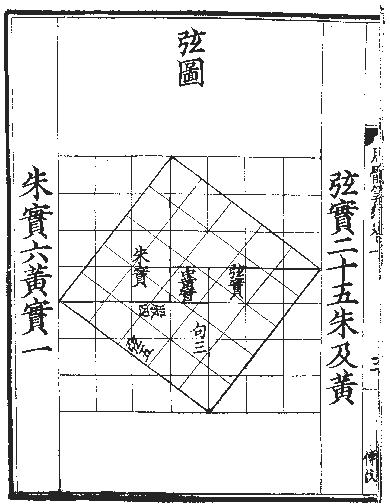
\includegraphics[height=\textheight-2\baselineskip]{xiantu-ancient.pdf}
  \caption{旧年做的雕版}
  \label{fig:xiantuancient}
\end{figure}
\begin{figure}
  \centering
  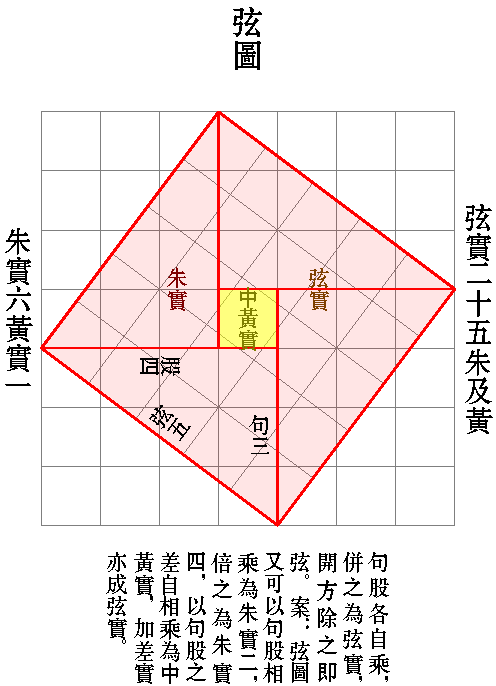
\includegraphics{xiantu.pdf}
  \caption{理想中的新版本}
  \label{fig:xiantu}
\end{figure}

计议已定,赵博士要开始正式的绘图了。

\section{绘图环境}

\Asy{} 的安装并不复杂,在 Windows 下面就是下载运行那个安装包,在 Linux 下面一
般也只需要下载对应的压缩包,解压就可以使用了。哦,赵博士用的就是 Windows。

点图标运行 \Asy{},就出现了交互式\index{交互式}的命令行,提示符是一个
\verb=>=。输入命令:
\begin{asycode}
draw((0,0) -- (3cm,4cm));   // `\color{comment}一条直线`
\end{asycode}
赵博士装的 GSView 立即弹了出来,里面已经画出一条倾斜的直线。再输入
|quit|\index{quit@\asyinline=quit=},程序退出,并留下了一个叫做
\verb=out.eps= 的图形文件,
小菜一碟。

这里稍稍解释一下上面的一句代码。|draw|\index{draw@\asyinline=draw=} 是画线的
命令,更准确地说,是 \Asy{} 中的函数\index{函数}:它带有一个参数\index{参数}
|(0,0) -- (3cm,4cm)|,参数外面是圆括号,整个命令以分号结束。里面的
|(0,0) -- (3cm,4cm)| 是由两个坐标\index{坐标}连接而成的直线,坐标是在直角坐标
系下的,可以带单位 |mm|, |cm|, |pt|, |bp|, |inch|, |inches|,%
\index{mm@\asyinline=mm=}\index{cm@\asyinline=cm=}\index{pt@\asyinline=pt=}%
\index{bp@\asyinline=bp=}\index{inch@\asyinline=inch=}%
\index{inches@\asyinline=inches=}%
其意义与在\TeX{} 中的一样,如果不带单位,则默认为 |bp|。行末以 |//| 开头的是
注释,另有一种在 |/* */| 之间的注释\index{注释},与 C 语言相同。

\index{编译}
不过赵博士写书讲求胸有成竹方才下笔,因此他更愿意使用更一种方式:打开一个文本
编辑器,把上面的绘图命令都录入完毕,保存为一个名为 \verb=line.asy= 的文件,最
后把这个文件拖动到 \Asy{} 的图标上面,就完成了整个作图。

赵博士的小侄子不屑于这种快捷图标的编译方式,他直接进入命令行,输入
\verb=asy=,就进入了 \Asy{} 的交互环境;要是输入 \verb=asy line=,就画出了刚
才的保存的直线。


\section{直线与绘图命令}
\label{sec:linedraw}

弦图的图形其实很简单,都是直线、方块、三角形这些,而且为了计算的简便,所有长
度也都是整数值。那么,首先就是在 \Asy{} 中来画直线。

\index{画线}
正如前面试验的时候做的那样,一条直线就是用 |--|\index{--@\asyinline=--=} 把坐
标连起来,再使用 |draw| 命令,直线就画出来了。事实上,可以用 |--| 把坐标点连
成折线:
\begin{asycode}
draw( (0,0) -- (1cm,0) -- (2cm,0.5cm) -- (1cm,1cm) -- (0,1cm) );
\end{asycode}
\begin{figure}[H]
\centering
\begin{asy}
draw( (0,0) -- (1cm,0) -- (2cm,0.5cm) -- (1cm,1cm) -- (0,1cm) );
\end{asy}
\end{figure}

像这样把坐标用 |--| 连结起来的,就成为一条路径\index{路径}。把直线而稍做修改
,在后面连上一个特殊的坐标 |cycle|\index{cycle@\asyinline=cycle=},就可以得到
一条首尾相接的闭路径\index{路径!闭路径}。如:
\begin{asycode}
draw( (0,0) -- (1cm,0) -- (2cm,0.5cm) -- (1cm,1cm) -- (0,1cm) -- cycle );
\end{asycode}
\begin{figure}[H]
\centering
\begin{asy}
draw( (0,0) -- (1cm,0) -- (2cm,0.5cm) -- (1cm,1cm) -- (0,1cm) -- cycle );
\end{asy}
\end{figure}

画一条路径可以使用不同的颜色、粗细的笔,这只要给 |draw| 命令多加一个画笔
\index{画笔}参数(多个参数用逗号分开):
\begin{asycode}
draw((0,0) -- (1cm,0) -- (2cm,0.5cm) -- (1cm,1cm) -- (0,1cm), darkblue+1mm);
\end{asycode}
\begin{figure}[H]
\centering
\begin{asy}
draw((0,0) -- (1cm,0) -- (2cm,0.5cm) -- (1cm,1cm) -- (0,1cm), darkblue+1mm);
\end{asy}
\end{figure}
这里 |darkblue| 是颜色,|1mm| 是线的粗细。|darkblue+1mm| 即指一毫米宽的深
蓝色粗线。(可用的颜色\index{颜色}名称可以参考 \cite{asyman})

赵博士画的是“勾三股四弦五”的红色三角形,这很容易:
\begin{asycode}
draw( (0,0) -- (4cm,0) -- (0,3cm) -- cycle, red+0.5mm );
\end{asycode}
\begin{figure}[H]
\centering
\begin{asy}
draw( (0,0) -- (4cm,0) -- (0,3cm) -- cycle, red+0.5mm );
\end{asy}
\end{figure}

\index{填充}
不过现在还需要的是实心的三角形,因此就需要一个新的绘图命令
|fill|\index{fill@\asyinline=fill=},即填充。于是,红色三角形就成为
\begin{asycode}
fill( (0,0) -- (4cm,0) -- (0,3cm) -- cycle, red );
\end{asycode}
\begin{figure}[H]
\centering
\begin{asy}
fill( (0,0) -- (4cm,0) -- (0,3cm) -- cycle, red );
\end{asy}
\end{figure}

但这样一来三角形的颜色就太重了,而且边界也不清楚。因此似乎应该先用浅红色填充
一遍,然后再用深红色勾边。好在可以使用一个命令
|filldraw|\index{filldraw@\asyinline=filldraw=} 同时完成这两件事情,这样就不
需要把一条路径写两遍了。即有:
\begin{asycode}
filldraw((0,0) -- (4cm,0) -- (0,3cm) -- cycle,
    fillpen=palered, drawpen=red+0.5mm);
\end{asycode}
\begin{figure}[H]
\centering
\begin{asy}
filldraw((0,0) -- (4cm,0) -- (0,3cm) -- cycle,
    fillpen=palered, drawpen=red+0.5mm);
\end{asy}
\end{figure}
这里可以简单地直接写两个参数 |palered, red+0.5mm|,不过为了清晰起见还是使用
“$\text{键}=\text{值}$”的写法,明确表示出填充的画笔和描线的画笔。

现在,赵博士的整个弦图的框架就呼之欲出了,就是画出四个三角形
(\autoref{fig:xiantuskeleton}):
\begin{asycode}
filldraw( (4cm,0) -- (4cm,3cm) -- (0,3cm) -- cycle,
    fillpen=palered, drawpen=red+0.5mm);
filldraw( (7cm,4cm) -- (4cm,4cm) -- (4cm,0) -- cycle,
    fillpen=palered, drawpen=red+0.5mm);
filldraw( (3cm,7cm) -- (3cm,4cm) -- (7cm,4cm) -- cycle,
    fillpen=palered, drawpen=red+0.5mm);
filldraw( (0,3cm) -- (3cm,3cm) -- (3cm,7cm) -- cycle,
    fillpen=palered, drawpen=red+0.5mm);
\end{asycode}
\begin{figure}
\centering
\begin{asy}
filldraw( (4cm,0) -- (4cm,3cm) -- (0,3cm) -- cycle,
    fillpen=palered, drawpen=red+0.5mm);
filldraw( (7cm,4cm) -- (4cm,4cm) -- (4cm,0) -- cycle,
    fillpen=palered, drawpen=red+0.5mm);
filldraw( (3cm,7cm) -- (3cm,4cm) -- (7cm,4cm) -- cycle,
    fillpen=palered, drawpen=red+0.5mm);
filldraw( (0,3cm) -- (3cm,3cm) -- (3cm,7cm) -- cycle,
    fillpen=palered, drawpen=red+0.5mm);
\end{asy}
\caption{弦图的初步框架}\label{fig:xiantuskeleton}
\end{figure}

还应该画出弦图的中间的“黄实”,用黄色填充。这部分是一个正方形,可以使用现成
的 \lstinline[language=Asymptote,mathescape]|box($\text{角点}$, $\text{角点}$)|
\index{box@\asyinline=box=} 命令来产生矩形的路径,因而填充正中间的正方形就可
以用:
\begin{asycode}
fill( box((3cm,3cm), (4cm,4cm)), yellow );
\end{asycode}
这个填充的命令应该放在画线之前(以免覆盖描的红线)。

回顾前面的代码,赵博士觉得连续地写四个 |filldraw| 命令太重复了。他读了 \Asy{}
的文档 \cite{asyman},才知道多条路径可以用符号 |^^|\index{^^@\asyinline=^^=} 
连起来,一起使用,于是立即着手改进原来的代码。

而且,由于还打算在图的后面画出参考网格,图形的颜色还应该设置为半透明\index{透
明}的。好在这并不难实现,只要稍稍改动一下填充的画笔,使用
\lstinline[language=Asymptote,mathescape]|opacity($\text{数值}$)|
\index{opacity@\asyinline=opacity=}
来设定有一定不透明度(取值为 $0\sim1$)的画笔,并把它加在原来的画笔上
\footnote{\Asy{} 的 EPS 格式输出看不到透明效果,必须输出为 PDF 格式或从 PDF 
格式转化为其他格式才能有透明效果。}。于是赵博士最后写出了这样的代码:
\begin{asycode}
fill( box((3cm,3cm), (4cm,4cm)), opacity(0.5)+yellow );
filldraw( (4cm,0) -- (4cm,3cm) -- (0,3cm) -- cycle
    ^^ (7cm,4cm) -- (4cm,4cm) -- (4cm,0) -- cycle
    ^^ (3cm,7cm) -- (3cm,4cm) -- (7cm,4cm) -- cycle
    ^^ (0,3cm) -- (3cm,3cm) -- (3cm,7cm) -- cycle,
    fillpen=opacity(0.1)+red, drawpen=red+0.5mm );
\end{asycode}
至此,弦图的主要框架(\autoref{fig:xiantuskeleton2})就此完成。
\begin{figure}[H]
\centering
\begin{asy}
fill( box((3cm,3cm), (4cm,4cm)), opacity(0.5)+yellow );
filldraw( (4cm,0) -- (4cm,3cm) -- (0,3cm) -- cycle
    ^^ (7cm,4cm) -- (4cm,4cm) -- (4cm,0) -- cycle
    ^^ (3cm,7cm) -- (3cm,4cm) -- (7cm,4cm) -- cycle
    ^^ (0,3cm) -- (3cm,3cm) -- (3cm,7cm) -- cycle,
    fillpen=opacity(0.1)+red, drawpen=red+0.5mm );
\end{asy}
\caption{弦图的进一步优化的框架}\label{fig:xiantuskeleton2}
\end{figure}


\section{图形变换与功能模块的使用}
\label{sec:transformmodule}

然后是画作为长度参考的网格。其实网格一开始就该在图中画出来,这样后面画图准确
与否才能看得清楚。不过现在赵博士是重作旧图,图样已定,网格就搁在弦图的主要图
形后面才画了。

按说这个网格是十分简单的,无非就是画一些灰色的纵横细线。比如这个 $3\times3$ 
的网格:
\begin{asycode}
draw( (0,0) -- (3cm,0)
    ^^ (0,1cm) -- (3cm,1cm)
    ^^ (0,2cm) -- (3cm,2cm)
    ^^ (0,3cm) -- (3cm,3cm),
    gray );
draw( (0,0) -- (0,3cm)
    ^^ (1cm,0) -- (1cm,3cm)
    ^^ (2cm,0) -- (2cm,3cm)
    ^^ (3cm,0) -- (3cm,3cm),
    gray );
\end{asycode}
\begin{figure}[H]
\centering
\begin{asy}
draw( (0,0) -- (3cm,0)
    ^^ (0,1cm) -- (3cm,1cm)
    ^^ (0,2cm) -- (3cm,2cm)
    ^^ (0,3cm) -- (3cm,3cm),
    gray );
draw( (0,0) -- (0,3cm)
    ^^ (1cm,0) -- (1cm,3cm)
    ^^ (2cm,0) -- (2cm,3cm)
    ^^ (3cm,0) -- (3cm,3cm),
    gray );
\end{asy}
\end{figure}

可无疑这个办法显得太麻烦了,赵博士要画的是 $7\times7$ 的网格,就要分别画出
$16$ 条直线。这样的代码不仅不好写,而且容易出错,修改一下也很麻烦。

赵博士看到了手册 \cite{asyman} 中讲循环语句的用法,似乎可以完成这件事。可是以
赵博士的年龄,再去看什么编程什么变量的,命令不能一条一条执行下来,很不习惯,
头脑就往往转不清楚。

\index{模块!math@\prgname{math}}
于是赵博士就去论坛上咨询,一些人劝他去用几行循环语句,甚至有人已经把完整的函
数做好了。但有一个结果特别引人注目,有人指出,在 \prgname{math} 模块中已经定
义好了一个 |grid| 函数,只要拿来用就可以了。赵博士立即精神大振,来看这个
|grid| 函数:\index{grid@\asyinline=grid=}
\begin{asycode}
picture grid(int Nx, int Ny, pen p=currentpen)
\end{asycode}
这个是在 \prgname{math} 模块中 |grid| 函数的原型。\index{原型}它说明 |grid| 
函数有 |Nx|, |Ny| 两个整数类型的必需参数,一个可选的画笔,并且返回一个
|picture|(图)\index{picture@\asyinline=picture=}类型的对象。

\index{导入}\index{模块!导入}
要使用模块的功能,需要在绘图之前导入这个模块,这只要使用
\index{import@\asyinline=import=}
\begin{asycode}
import `模块名`;
\end{asycode}
因此,要使用 \prgname{math} 模块中的 |grid| 函数,只要在代码中写
\begin{asycode}
import math;
\end{asycode}
就可以了。

|grid| 函数的行为看起来很奇怪,调用它会在一个单独的图上画出一个
|Nx|${}\times{}$|Ny| 的网格,网格的左下角在原点,间距为 $1$。要使用 |grid| 函
数画的图形,要使用 \lstinline[language=Asymptote,mathescape]|add($\text{图}$)|
\index{add@\asyinline=add=} 命令,把这个图形加在当前的图上:
\begin{asycode}
import math;
add(grid(10,10,gray));
\end{asycode}
\begin{figure}[H]
\centering
\begin{asy}
import math;
add(grid(10,10,gray));
\end{asy}
\end{figure}
不过直接这样做的结果是只能得到一个小得已经看不清的网格。因此,必须对图形进行放缩。

\index{变换}\index{仿射变换}
\index{变换!平移}\index{变换!旋转}\index{变换!放缩}
\index{变换!错切}\index{变换!反射}
\Asy{} 提供了平移、旋转、放缩、倾斜、反射等各种的仿射变换,来对坐标、路径、图
形等元素进行变换(严格的函数原型参考 \cite{asyman}):
\index{shift@\asyinline=shift=}
\index{scale@\asyinline=scale=}
\index{xscale@\asyinline=xscale=}
\index{yscale@\asyinline=yscale=}
\index{rotate@\asyinline=rotate=}
\index{slant@\asyinline=slant=}
\index{reflect@\asyinline=reflect=}
\begin{asycode}
shift(`坐标`)           // `\color{comment}按坐标平移`
shift(x, y)           // `\color{comment}按` (x, y) `\color{comment}平移`
scale(`倍数`)           // `\color{comment}按倍数放缩`
xscale(`倍数`)          // `\color{comment}$x$ 轴方向按倍数放缩`
yscale(`倍数`)          // `\color{comment}$y$ 轴方向按倍数放缩`
scale(x, y)           // `\color{comment}在 $x$ 轴、$y$ 轴方向分别按倍数` x, y `\color{comment}放缩`
rotate(`角度`, z=(0,0)) // `\color{comment}按角度绕中心` z`\color{comment}(默认为原点,逆时针)旋转`
slant(`因子`)           // `\color{comment}按一定因子向右倾斜`
reflect(a, b)         // `\color{comment}相对直线` a--b `\color{comment}反射`
\end{asycode}
使用一个变换就是把这个变换乘在被变换对象的左边。例如一个放缩一个单位正方形:
\begin{asycode}
draw( scale(2cm) * box((0,0), (1,1)) );
\end{asycode}
\begin{figure}[H]
\centering
\begin{asy}
draw( scale(2cm) * box((0,0), (1,1)) );
\end{asy}
\end{figure}
这样的变换可以连续地做下去,例如
\begin{asycode}
draw( rotate(90) * slant(0.3) * scale(1cm) * box((0,0), (1,1)) );
\end{asycode}
就是把一个单位正方形先放大,再倾斜,再旋转 $90^\circ$:
\begin{figure}[H]
\centering
\begin{asy}
draw( rotate(90) * slant(0.3) * scale(1cm) * box((0,0), (1,1)) );
\end{asy}
\end{figure}

有了这些变换,画出一个合适大小的网格就不再是什么难事了:
\begin{asycode}
import math;
add( scale(5mm) * grid(4, 4, gray) );
\end{asycode}
\begin{figure}[H]
\centering
\begin{asy}
import math;
add( scale(5mm) * grid(4, 4, gray) );
\end{asy}
\end{figure}

赵博士的弦图有两个网格,不仅要大小合适,而且其中一个需要进行旋转和平移。平移
的位置很明显,但旋转仍然需要一些计算。当然这难不倒精研天文算学多年的赵博士,
这里弦实($5\times5$ 的正方形)可以看作是顺时针旋转得到的,从朱实的三角形容易
看出旋转的角度正好是 $\arctan(3/4)$。\Asy{} 中也可以方便地调用返回角度的反三
角函数 |aTan|\index{aTan@\asyinline=aTan=} 来计算这个角度\footnote{也可以使用
atan2 函数,但注意返回值是弧度。}。更详细的数学函数列表,参看 \cite{asyman}。
(注意:C/C++ 中 |3/4| 表示求带余除法 $3\div 4$ 的商,得到 $0$;但在 \Asy{} 中
|3/4| 的结果是实数 $0.75$,整数的带余除法则用 |quotient(a,b)|
\index{quotient@\asyinline=quotient=} 函数。)

于是,赵博士弦图中的网格,就可以这样方便地画出来了
(\autoref{fig:xiantugrid}):
\begin{asycode}
// `\color{comment}网格`
import math;
add( scale(1cm) * grid(7, 7, gray) );
add( shift(0,3cm) * rotate(-aTan(3/4)) * scale(1cm) * grid(5, 5, gray) );
// `\color{comment}弦图主体`
fill( box((3cm,3cm), (4cm,4cm)), opacity(0.5)+yellow );
filldraw( (4cm,0) -- (4cm,3cm) -- (0,3cm) -- cycle
    ^^ (7cm,4cm) -- (4cm,4cm) -- (4cm,0) -- cycle
    ^^ (3cm,7cm) -- (3cm,4cm) -- (7cm,4cm) -- cycle
    ^^ (0,3cm) -- (3cm,3cm) -- (3cm,7cm) -- cycle,
    fillpen=opacity(0.1)+red, drawpen=red+0.5mm );
\end{asycode}
\begin{figure}[htbp]
\centering
\begin{asy}
// 网格
import math;
add( scale(1cm) * grid(7, 7, gray) );
add( shift(0,3cm) * rotate(-aTan(3/4)) * scale(1cm) * grid(5, 5, gray) );
// 弦图主体
fill( box((3cm,3cm), (4cm,4cm)), opacity(0.5)+yellow );
filldraw( (4cm,0) -- (4cm,3cm) -- (0,3cm) -- cycle
    ^^ (7cm,4cm) -- (4cm,4cm) -- (4cm,0) -- cycle
    ^^ (3cm,7cm) -- (3cm,4cm) -- (7cm,4cm) -- cycle
    ^^ (0,3cm) -- (3cm,3cm) -- (3cm,7cm) -- cycle,
    fillpen=opacity(0.1)+red, drawpen=red+0.5mm );
\end{asy}
\caption{带网格的弦图草图}
\label{fig:xiantugrid}
\end{figure}


\section{标注文字}

\index{标注}\index{标签}
现在要进行的是文字的标注。按照勾股定理的约定,赵博士打算在一个红色三角形内标
注“朱实”,在黄色矩形处标注“黄实”,并为拼得的整个大矩形标注“弦实”;在另
一红色三角形的三边标注“勾三”、“股四”、“弦五”的尺寸;最后在图形两侧加上
说明的文字。

在标注文字之前,对于中文标签\index{标签!中文标签},应该先定义好中文环境和字体
。\Asy{} 会调用 \LaTeX{} 来进行标签的处理,因而需要设置的就是 \LaTeX{} 的编译
引擎\index{LaTeX@\LaTeX!引擎}与一般的中文 \LaTeX{} 文件导言区。在这里,赵博士决定使
用 \XeTeX{}\index{XeTeX@\XeTeX} 引擎与
\prgname{xeCJK}\index{xeCJK@\prgname{xeCJK}} 宏包来处理中文。为此,在 \Asy{} 
源文件中,他使用了下面的设置代码:
\begin{asycode}
settings.tex = "xelatex";
usepackage("xeCJK");
texpreamble("\setCJKmainfont{SimSun}");
\end{asycode}
这里第一行是设置编译时所用的 \TeX{} 引擎。后面
|usepackage|\index{usepackage@\asyinline=usepackage=} 命令就是 \LaTeX{} 中的
\verb|\usepackage| 命令的一个包装形式,里面的字符串参数就是宏包名;而
|texpreamble|\index{texpreamble@\asyinline=texpreamble=} 命令则把接收的参数直
接放进 \LaTeX{} 的导言区。

进行上述设置后,就可以正确使用中文标签了。标注的命令很简单,就是
|label|\index{label@\asyinline=label=},参数正是标签文字和标签的位置。例如:
\begin{asycode}
draw( (0,0) -- (1cm,1cm) -- (2cm,0) );
label( "`\color{string}中间`", (1cm,0cm) );
\end{asycode}
就得到
\begin{figure}[H]
\centering
\begin{asy}
settings.tex = "xelatex";
usepackage("xeCJK");
texpreamble("\setCJKmainfont{SimSun}");
draw( (0,0) -- (1cm,1cm) -- (2cm,0) );
label( "中间", (1cm,0cm) );
\end{asy}
\end{figure}

可以在标签中使用任意的 \LaTeX{} 代码,包括数学公式,例如:
\begin{asycode}
label("$x = \sin\alpha$", (0,0));
\end{asycode}
就会正确地得到 $x = \sin\alpha$ 的标签。

现在,我们可以给弦图加上“朱实”、“黄实”和“弦实”的标签了。在前面的框架代
码后面加上
\begin{asycode}
label("`\color{string}朱实`", (2cm,4cm));
label("`\color{string}黄实`", (3.5cm,3.5cm));
label("`\color{string}弦实`", (5cm,4cm));
\end{asycode}
以及设置字体的代码,就得到\autoref{fig:xiantupartlabel} 的结果。
\begin{figure}
\centering
\begin{asy}
settings.tex = "xelatex";
usepackage("xeCJK");
texpreamble("\setCJKmainfont{SimSun}");
import math;
add( scale(1cm) * grid(7, 7, gray) );
add( shift(0,3cm) * rotate(-aTan(3/4)) * scale(1cm) * grid(5, 5, gray) );
fill( box((3cm,3cm), (4cm,4cm)), opacity(0.5)+yellow );
filldraw( (4cm,0) -- (4cm,3cm) -- (0,3cm) -- cycle
    ^^ (7cm,4cm) -- (4cm,4cm) -- (4cm,0) -- cycle
    ^^ (3cm,7cm) -- (3cm,4cm) -- (7cm,4cm) -- cycle
    ^^ (0,3cm) -- (3cm,3cm) -- (3cm,7cm) -- cycle,
    fillpen=opacity(0.1)+red, drawpen=red+0.5mm );
label("朱实", (2cm,4cm));
label("黄实", (3.5cm,3.5cm));
label("弦实", (5cm,4cm));
\end{asy}
\caption{带部分标注的弦图}\label{fig:xiantupartlabel}
\end{figure}

下面则是要给三角形的三边进行标注。

\index{标签!路径上的标签}
与前面在一个点处标注不同,这里实际是给一条路径(直线)标注标签。因此,想要得
到的是距离这条路径的中点一定方向距离加一个标签,而不是简单地取路径上的一点作
为标签的位置。好在 \Asy{} 确实也提供了这样的功能,仍然使用 |label| 命令,基本
语法是:\index{label@\asyinline=label=}
\begin{asycode}
label(`标签`, `路径`)
\end{asycode}
这里默认会在路径中间的右侧(沿着路径行进方向)加标签。例如:
\begin{asycode}
draw( (0,0) -- (4cm,2cm), linewidth(0.5mm) );
label("`\color{string}粗线条`", (0,0) -- (4cm,2cm));
\end{asycode}
(其中的 |linewidth|\index{linewidth@\asyinline=linewidth=} 函数用来表示具有
一定线宽\index{线宽}的画笔)这段代码将得到
\begin{figure}[H]
\centering
\begin{asy}
settings.tex = "xelatex";
usepackage("xeCJK");
texpreamble("\setCJKmainfont{SimSun}");
draw( (0,0) -- (4cm,2cm), linewidth(0.5mm) );
label("粗线条", (0,0) -- (4cm,2cm));
\end{asy}
\end{figure}

现在,赵博士就可以给三角形的三边加上“勾三”、“股四”、“弦五”的标签了,只
要稍稍注意一下标签摆放的默认方向:
\begin{asycode}
filldraw( (4cm,0) -- (4cm,3cm) -- (0,3cm) -- cycle,
    fillpen=opacity(0.1)+red, drawpen=red+0.5mm );
label( "`\color{string}勾三`", (4cm,3cm) -- (4cm,0) );
label( "`\color{string}股四`", (0,3cm) -- (4cm,3cm) );
label( "`\color{string}弦五`", (4cm,0) -- (0,3cm) );
\end{asycode}
\begin{figure}[H]
\centering
\begin{asy}
settings.tex = "xelatex";
usepackage("xeCJK");
texpreamble("\setCJKmainfont{SimSun}");
filldraw( (4cm,0) -- (4cm,3cm) -- (0,3cm) -- cycle,
    fillpen=opacity(0.1)+red, drawpen=red+0.5mm );
label( "勾三", (4cm,3cm) -- (4cm,0) );
label( "股四", (0,3cm) -- (4cm,3cm) );
label( "弦五", (4cm,0) -- (0,3cm) );
\end{asy}
\end{figure}

不过,为了得到正确的标签位置,不得不把原来逆时针画的线用顺时针方向重写,这多
少让赵博士有些恼火:为什么不能在路径的左边标注标签呢?确实可以,很简单,只要
给 |label| 命令再加上 |align=LeftSide|\index{align@\asyinline=align=}
\index{LeftSide@\asyinline=LeftSide=} 选项(或者简单地只用 |LeftSide|)就指定
了在左边放置对齐。同理,还有向右对齐的
|RightSide|\index{RightSide@\asyinline=RightSide=},在中间对齐的
|Center|\index{Center@\asyinline=Center=} 以及一般意义的相对方向
\lstinline[language=Asymptote,mathescape]|Relative($\text{方向}$)|。%
\index{Relative@\asyinline=Relative=}%
例如:
\begin{asycode}
draw( (0,0) -- (4cm,2cm), blue, Arrow );
label( "LeftSide", (0,0) -- (4cm,2cm), align=LeftSide );
label( "RightSide", (0,0) -- (4cm,2cm), align=RightSide );
label( "Center", (0,0) -- (4cm,2cm), align=Center );

draw( (6cm,0)--(8cm,2cm), blue, Arrow );
label( "E", (6cm,0)--(8cm,2cm), Relative(E) );
label( "S", (6cm,0)--(8cm,2cm), Relative(S) );
label( "W", (6cm,0)--(8cm,2cm), Relative(W) );
label( "N", (6cm,0)--(8cm,2cm), Relative(N) );
\end{asycode}
\begin{figure}[H]
\centering
\begin{asy}
draw( (0,0) -- (4cm,2cm), blue, Arrow );
label( "LeftSide", (0,0) -- (4cm,2cm), align=LeftSide );
label( "RightSide", (0,0) -- (4cm,2cm), align=RightSide );
label( "Center", (0,0) -- (4cm,2cm), align=Center );

draw( (6cm,0)--(8cm,2cm), blue, Arrow );
label( "E", (6cm,0)--(8cm,2cm), Relative(E) );
label( "S", (6cm,0)--(8cm,2cm), Relative(S) );
label( "W", (6cm,0)--(8cm,2cm), Relative(W) );
label( "N", (6cm,0)--(8cm,2cm), Relative(N) );
\end{asy}
\end{figure}
|E|, |S|, |W|, |N|\index{E@\asyinline=E=}\index{S@\asyinline=S=}
\index{W@\asyinline=W=}\index{N@\asyinline=N=} 分别是东南西北四个罗盘方向,%
\index{罗盘方向}用在 |Relative| 函数里面就表示相对于路径方向的四个方向。为明
确,这里用 |Arrow|\index{Arrow@\asyinline=Arrow=} 选项在画线时加了箭头。
\index{箭头}

不过,这样的标签还是不能令赵博士满意。赵博士给三角形加标签,还希望标签随着三
角形的边作旋转,使标签沿着边排列。为此,赵博士不得不又仔细查看了
\cite{asyman},在讲标注文字一节(label)他找到了一个构造标签的更高级的办法,
即不仅仅是使用一个简单的字符串,而是使用\index{Label@\asyinline=Label=}
\begin{asycode}
Label(`标签`)
\end{asycode}
函数进行构造。里面的“标签”参数仍然可以是原来的字符串,或是通过这个函数构造
出来的高级的标签。这个函数可以带许多可选的其他参数,如
\lstinline[language=Asymptote,mathescape]|position=$\text{位置}$|
\index{position@\asyinline=position=} 的参数就可以指定标签放在路径中点之外的
其他地方;而 \lstinline[language=Asymptote,mathescape]|embed=$\text{嵌入变换方式}$|
\index{embed@\asyinline=embed=} 的参数则可以解决标签自动旋转的问题。

这里暂且放下 |position| 参数。只来看 |embed| 参数的一个特例:%
\lstinline[language=Asymptote,mathescape]|Rotate($\text{方向}$)|%
\index{Rotate@\asyinline=Rotate=}。这个参数会让标签向着给定的方向旋转,如:
\begin{asycode}
draw( (0,0)--(4cm,2cm), blue, Arrow );
label( Label("Rotate", Rotate((4,2))),
    (0,0)--(4cm,2cm) );
\end{asycode}
\begin{figure}[H]
\centering
\begin{asy}
draw( (0,0)--(4cm,2cm), blue, Arrow );
label( Label("Rotate", Rotate((4,2))),
    (0,0)--(4cm,2cm) );
\end{asy}
\end{figure}
这里坐标 $(4,2)$ 正是这条直线的绘制方向。

终于,使用了上面的全部功能,赵博士完成了全部的图形标注工作
(\autoref{fig:xiantulabel}):
\begin{asycode}
settings.tex = "xelatex";
usepackage("xeCJK");
texpreamble("\setCJKmainfont{SimSun}");

import math;
add( scale(1cm) * grid(7, 7, gray) );
add( shift(0,3cm) * rotate(-aTan(3/4)) * scale(1cm) * grid(5, 5, gray) );

fill( box((3cm,3cm), (4cm,4cm)), opacity(0.5)+yellow );
filldraw( (4cm,0) -- (4cm,3cm) -- (0,3cm) -- cycle
    ^^ (7cm,4cm) -- (4cm,4cm) -- (4cm,0) -- cycle
    ^^ (3cm,7cm) -- (3cm,4cm) -- (7cm,4cm) -- cycle
    ^^ (0,3cm) -- (3cm,3cm) -- (3cm,7cm) -- cycle,
    fillpen=opacity(0.1)+red, drawpen=red+0.5mm );

label("`\color{string}朱实`", (2cm,4cm));
label("`\color{string}黄实`", (3.5cm,3.5cm));
label("`\color{string}弦实`", (5cm,4cm));
label( Label("`\color{string}勾三`",Rotate(S)), (4cm,0)--(4cm,3cm), LeftSide );
label( Label("`\color{string}股四`",Rotate(E)), (4cm,3cm)--(0,3cm), LeftSide );
label( Label("`\color{string}弦五`",Rotate((4,-3))), (0,3cm)--(4cm,0), LeftSide );
\end{asycode}
\begin{figure}[htbp]
\centering
\begin{asy}
settings.tex = "xelatex";
usepackage("xeCJK");
texpreamble("\setCJKmainfont{SimSun}");

import math;
add( scale(1cm) * grid(7, 7, gray) );
add( shift(0,3cm) * rotate(-aTan(3/4)) * scale(1cm) * grid(5, 5, gray) );

fill( box((3cm,3cm), (4cm,4cm)), opacity(0.5)+yellow );
filldraw( (4cm,0) -- (4cm,3cm) -- (0,3cm) -- cycle
    ^^ (7cm,4cm) -- (4cm,4cm) -- (4cm,0) -- cycle
    ^^ (3cm,7cm) -- (3cm,4cm) -- (7cm,4cm) -- cycle
    ^^ (0,3cm) -- (3cm,3cm) -- (3cm,7cm) -- cycle,
    fillpen=opacity(0.1)+red, drawpen=red+0.5mm );

label("朱实", (2cm,4cm));
label("黄实", (3.5cm,3.5cm));
label("弦实", (5cm,4cm));
label( Label("勾三",Rotate(S)), (4cm,0)--(4cm,3cm), LeftSide );
label( Label("股四",Rotate(E)), (4cm,3cm)--(0,3cm), LeftSide );
label( Label("弦五",Rotate((4,-3))), (0,3cm)--(4cm,0), LeftSide );
\end{asy}
\caption{带标注的完整弦图}
\label{fig:xiantulabel}
\end{figure}


\section{习题和评注}

\begin{enumerate}
  \item 查阅参考手册 \cite{asyman},看看都有哪些颜色可用。看看你的系统中安装
    了哪些中文字体。然后修改\autoref{fig:xiantulabel},使用另一种你喜欢的字体
    进行标注;并且将“朱实”、“黄实”和“弦实”分别用红、黄、橙色标注。

  \item 查阅参考手册 \cite{asyman},看看 |draw|、|fill|、|label| 等命令都可以
    带哪些可选的参数,并自己举例子试验一下效果。

  \item 代码
\begin{asycode}
guide zhushi = (4cm,0) -- (4cm,3cm) -- (0,3cm) -- cycle;
\end{asycode}
    可以把一个三角形的路径保存在变量 |zhushi| 中,以后就可以使用
    |draw(zhushi)| 这样的命令对此路径进行操作了\footnote{这里定义了一个
    \asyinline=guide= 类型的变量,我们译之为“路向”,以区别于“路径”
    (\asyinline=path=)。两个概念在 \Asy{} 中同源而有别,但本章中二者可以互
    换并无区别,因此为方便我们也不区别而通称为路径。有关 \Asy{} 语言中路径与
    路向的区别,以及关于变量定义和使用的详细内容,请参考后续的章节及手册
    \cite{asyman}。}。

    考虑如何利用平移和旋转变换,只定义一个三角形的路径,就把弦图中的四个红色
    三角形都画出来。

  \item\label{ex:roundedpath} 查阅手册 \cite{asyman} 和 \Asy{} 自带的例子,研
    究模块
    \prgname{roundedpath}\index{模块!roundedpath@\prgname{roundedpath}} 的用
    法。并利用它尝试画出下面的图形:
\begin{figure}[H]
\centering
\begin{asy}
import roundedpath;
pen thick = linewidth(0.8pt);
guide p = (0,0) -- (0,2cm) -- (1cm,3.25cm) -- (2cm,2cm) -- (2cm,0)
	-- (0,2cm) -- (2cm, 2cm) -- (0,0) -- (2cm,0);
draw(roundedpath(p, 8pt), thick);
\end{asy}
\end{figure}

    看看 \Asy{} 中还有什么用法简单而又有趣的模块。

  \item (较难)研究在 \LaTeX{} 里中文直排的方法,尽量精确地复现出赵博士理想
    中的弦图效果(\autoref{fig:xiantu})。
\end{enumerate}

本章的素材源自有关我国古代对勾股定理证明的一篇介绍性论文 \cite{quanjing}。本
章的主要内容是 \Asy{} 中直线几何图形的基本绘制方法。有关平面几何的数学图形是
\Asy{} 以及 \MP{} 的传统长项和最重要的应用范围之一。不过 \Asy{} 默认自动加载
的 \prgname{plain} 模块功能比较原始,用来绘制平面几何图形往往比较麻烦,使用
由 Philippe Ivaldi 开发的专门模块 \prgname{geometry}
\index{模块!geometry@\prgname{geometry}}可以更容易地画出各种 Euclid 平面几何
的数学图形来,可参考此模块的英文文档 \cite{geometry}。

熟悉 C/C++ 语言的读者须注意,为了方便 \TeX{} 指令在 \Asy{} 中的书写,\Asy{} 
中的字符串内可以直接使用换行符,而不必手工使用转义符;另外,双引号内的字符串
只有 |\\| 和 |\"| 两种转义符,单引号也用来表示字符串,使用的转才与 C/C++ 语言
相同。

习题 \ref{ex:roundedpath} 的素材源自 \prgname{\textsc{pgf}/Ti\emph{k}Z} 宏包
的文档 \cite{pgfman}。\prgname{\textsc{pgf}/Ti\emph{k}Z} 宏包是基于 \TeX{} 的
绘图宏包,功能强大,一些方面更胜于老牌的 \prgname{PSTricks} 宏包。

\endinput

% vim:tw=77:


%# -*- coding: utf-8 -*-
% tiling.tex
% asymptotebyexample 的一章,曲线绘制和编程入门

\chapter{André Deledicq 的铺砌插画}
\nocite{pstricks}

André 是一名兴趣广泛的法国数学教师,在他的新著《Le monde des pavages》(《铺
砌世界》)中,打算画一幅有关羊的铺砌插画:
\begin{figure}[H]
  \centering
  
\includegraphics{tiling.pdf}
  \caption{André 理想中的铺砌图}
  \label{fig:tiling}
\end{figure}

André 很清楚他要画的图形的数学理论,但 André 的朋友 Timothy 告诉他要画这样
的图形多少是需要一些编程的知识的,对于他这样一位往日对计算机并不通晓的人来说
可能会有困难。不过 André 并不以为意:这世上还有什么比数学更难的呢?于是他兴
致勃勃的开始了。

\section{从矩形到铺砌}
\label{sec:rect2tiling}

铺砌图,顾名思义,就是像铺地板砖一样,把许多相同样式的图形平铺开来。不过,并
不是什么图形都可以平铺填满整个平面的——比如圆形就不行。把许多圆形一个挨一个
排列起来,也只能得到
\begin{figure}[H]
\centering
\begin{asy}
size(0,2cm);
for (int i = 0; i < 3; ++i)
    for (int j = 0; j < 10; ++j)
        filldraw(circle((j,i), 0.5), lightblue);
\end{asy}
\end{figure}
\noindent 或者是
\begin{figure}[H]
\centering
\begin{asy}
size(0,2cm);
for (int i = 0; i < 3; ++i)
    for (int j = 0; j < 10; ++j)
        filldraw(circle((j+0.5(i%2),sqrt(3)/2*i), 0.5), lightblue);
\end{asy}
\end{figure}
\noindent 都会留下许多空隙。而矩形、平行四边形、六边形等等都可以不留空隙地把平面铺满。

但问题是,如何设计出 André 理想中的那种看起来形状不规则的铺砌图案呢?

身为数学教师的 André 当然有办法。其实不规则铺砌图案还是规则图案的变形。
André 要画的羊形铺砌图,其实就是从矩形铺砌变化而来的。只要把一个矩形图案的上
下两边、左右两边分别变形,使得变形后的上边与下边、左边与右边还对应重合,就依
然可以完美地拼合起来。这正是铺砌图案最基本的构成方式:
\begin{figure}[H]
\centering
\begin{asy}
size(0,5cm);
defaultpen(linewidth(1mm));
guide rec = box((0,0), (2,1));
draw(rec);

draw(shift(3,0)*rec, gray+0.5mm);
guide left = (0,1) -- (-0.2,0.8) -- (0,0.6) -- (0.1,0.1) -- (0,0);
guide bot = (0,0) -- (0.2,0.1) -- (1.6,-0.1) -- (2,0);
draw(shift(3,0) * (left ^^ shift(2,0)*left), heavyblue);
draw(shift(3,0) * (bot ^^ shift(0,1)*bot), heavygreen);

guide shape = left & bot & shift(2,0)*reverse(left)
    & shift(0,1)*reverse(bot) & cycle;
for (int i = 0 ; i < 2; ++i)
    for (int j = 0; j < 4; ++j)
	filldraw(shift(0.5+j,-1.5+0.5i)*scale(0.5)*shape, lightblue);
\end{asy}
\end{figure}

有了这个方法,对复杂的铺砌图,也只要从一个基本形状(比如矩形、正六边形)开始
变形,就等到铺砌所需要的一块“砖”。

因此,要画出羊头形状铺砌图,只要把一个矩形按照上面的要求变形为一个羊头形状,
在不同的位置重复画出就可以了。

\section{变量与曲线}

下面的问题就是,怎么画一个羊头呢?更具体地说,怎么画出羊头的曲线呢?

那么,首先要了解如何在 \Asy{} 中描述曲线。\ref{sec:linedraw} 节中提到 |--| 连
结一组坐标就成为直(折)线段;类似地,用 |..|\index{..@\lstinline=..=} 连结坐
标就得到经过这些坐标点的曲线:
\begin{lstlisting}
size(5cm,0);
pair z1 = (0,1), z2 = (1,1), z3 = (2,1),
     z4 = (0,0), z5 = (1,0), z6 = (2,0);
guide p = z4 .. z1 .. z2 .. z6;
draw(p, gray+2mm);
\end{lstlisting}
\begin{figure}[H]
  \centering
\begin{asy}
size(5cm,0);
pair z1 = (0,1), z2 = (1,1), z3 = (2,1),
     z4 = (0,0), z5 = (1,0), z6 = (2,0);
guide p = z4 .. z1 .. z2 .. z6;
draw(p, gray+2mm);
dot(Label("1", align=NW), z1);
dot(Label("2", align=NE), z2);
dot("3", z3);
dot("4", z4);
dot("5", z5);
dot("6", z6);
\end{asy}
\end{figure}

在这里,我们定义了一些变量\index{变量}以使代码清晰(这里略去了画点和标签的代
码)。|pair|\index{pair@\lstinline=pair=} 类型的变量 |z1|, \ldots, |z6| 保存
六个坐标\index{坐标},|guide|\index{guide@\lstinline=guide=} 类型的变量 |p| 
保存一条曲线的路向\index{路向}。因而上面 |size| 之后的绘图代码就相当于
\begin{lstlisting}
draw( (0,0) .. (0,1) .. (1,1) .. (2,0), gray+2mm );
\end{lstlisting}
其中前面的一句 |size(5cm,0)|\index{size@\lstinline=size=} 表示代码中的坐标只
是相对位置,最后将整个图形按比例放缩为 $5$\,cm 宽\footnote{注意坐标、图形会被
放缩,但画笔的宽度不会放缩。}。类似地,也可以使用 |size(0,4cm)| 把图形放缩到
$4$\,cm 高。

最重要的当然还是曲线的表示。以 |..| 连结的坐标会以一种尽量接近圆弧的方式连为
经过这些点的光滑曲线。与画直线类似,|cycle|\index{cycle@\lstinline=cycle=} 可
以作为一个特殊的坐标产生闭合曲线,即一条闭路向\index{路向!闭路向}:
\begin{lstlisting}
guide q = z4 .. z1 .. z2 .. z6 .. cycle;
draw(q, gray+2mm);
\end{lstlisting}
\begin{figure}[H]
  \centering
\begin{asy}
size(5cm,0);
pair z1 = (0,1), z2 = (1,1), z3 = (2,1),
     z4 = (0,0), z5 = (1,0), z6 = (2,0);
guide q = z4 .. z1 .. z2 .. z6 .. cycle;
draw(q, gray+2mm);
dot(Label("1", align=NW), z1);
dot(Label("2", align=NE), z2);
dot("3", z3);
dot("4", z4);
dot("5", z5);
dot("6", z6);
\end{asy}
\end{figure}

变量不仅仅是给了坐标、路向等对象一个简洁的名字,它也使得对同一个对象重复使用
并进行不同的操作变得十分方便:
\begin{lstlisting}
fill(q, lightblue);
draw(q, gray+2mm);
\end{lstlisting}
\begin{figure}[H]
  \centering
\begin{asy}
size(5cm,0);
pair z1 = (0,1), z2 = (1,1), z3 = (2,1),
     z4 = (0,0), z5 = (1,0), z6 = (2,0);
guide q = z4 .. z1 .. z2 .. z6 .. cycle;
fill(q, lightblue);
draw(q, gray+2mm);
dot(Label("1", align=NW), z1);
dot(Label("2", align=NE), z2);
dot("3", z3);
dot("4", z4);
dot("5", z5);
dot("6", z6);
\end{asy}
\end{figure}

就像使用 |box| 可以直接得到矩形一样,最常用的曲线:圆、椭圆和圆弧,也可以使用
现成的命令得到:
\begin{table}[H]
\noindent
\begin{tabular}{ll}
|circle(c, r)| & 圆心 |c|,半径 |r| 的圆,这是逆时针方向的闭曲线; \\
|ellipse(c, a, b)| & 中心为 |c|,长半轴 |a|,短半轴 |b| 的椭圆,这也是逆时针
方向的闭曲线; \\
|arc(c, r, angle1, angle2)| & 圆心 |c|,半径 |r|,角度从 |angle1| 到 |angle2|
的圆弧。
\end{tabular}
\end{table}

例如:
\begin{lstlisting}
filldraw( circle((0,0), 1cm), lightblue, gray+2mm );
draw( arc((5cm,0), 1cm, 45, 135), gray+2mm );
\end{lstlisting}
\begin{figure}[H]
\centering
\begin{asy}
filldraw( circle((0,0), 1cm), lightblue, gray+2mm );
draw( arc((5cm,0), 1cm, 45, 135), gray+2mm );
\end{asy}
\end{figure}

一条用 |cycle| 产生的闭路向和简单地把首尾结点重合的路向是非常不同的。首先,只
有闭路向可以填充颜色;其次,使用 |cycle| 连结的曲线在起点处是光滑连接的,而如
果只是首尾结点重合则不会光滑连接。试将下面的曲线 |q2| 与上面的曲线 |q| 比较:
\begin{lstlisting}
guide q2 = z4 .. z1 .. z2 .. z6 .. z4;
draw(q2, gray+2mm);
\end{lstlisting}
\begin{figure}[H]
\centering
\begin{asy}
size(5cm,0);
pair z1 = (0,1), z2 = (1,1), z3 = (2,1),
     z4 = (0,0), z5 = (1,0), z6 = (2,0);
guide q2 = z4 .. z1 .. z2 .. z6 .. z4;
draw(q2, gray+2mm);
dot(Label("1", align=NW), z1);
dot(Label("2", align=NE), z2);
dot("3", z3);
dot("4", z4);
dot("5", z5);
dot("6", z6);
\end{asy}
\end{figure}

现在有了绘制曲线的方法,画出一个羊头就只是把草稿上的坐标连接起来而已。André
有一个纸上的草图,于是在描出几个点以后,他很快得到这样的结果(这里给图形增加
了辅助网格):
\begin{lstlisting}
size(0,4cm);
pen outline = black+1mm;
// `\color{comment}头`
guide head = (0.5,-0.2) .. (0.6,0.5) .. (0.2,1.3) .. (0,1.5) .. (0,1.5)
    .. (0.4,1.3) .. (0.8,1.5) .. (2.2,1.9) .. (3,1.5) .. (3.2,1.3)
    .. (3.6,0.5) .. (3.4,-0.3) .. (3,0) .. (2.2,0.4) .. (0.5,-0.2) .. cycle;
filldraw(head, cyan, outline);
dot(head, red+1mm); // `\color{comment}画出羊头曲线上的结点`
// `\color{comment}五官`
fill( circle((2.65,1.25), 0.12), outline );
fill( (3.5,0.3) .. (3.35,0.45) .. (3.5,0.6) .. (3.6,0.4) .. cycle, outline );
draw( (3,0.35) .. (3.3,0.1) .. (3.6,0.05), outline );
draw( (2.3,1.3) .. (2.1, 1.5) .. (2.15,1.7), outline );
draw( (2.1,1.7) .. (2.35,1.6) .. (2.45,1.4), outline );
\end{lstlisting}
\begin{figure}[H]
  \centering
\begin{asy}
size(0,4cm);
import math;
add(scale(1/2)*shift(0,-1)*grid(8,5,gray));
dot(Label("$O$",align=left), 0);
label("$1$", (0,1), align=W); label("$2$", (0,2), align=W);
label("$1$", (1,-0.5), align=S); label("$2$", (2,-0.5), align=S);
label("$3$", (3,-0.5), align=S); label("$4$", (4,-0.5), align=S);
pen outline = black+1mm;
guide head = (0.5,-0.2) .. (0.6,0.5) .. (0.2,1.3) .. (0,1.5) .. (0,1.5)
    .. (0.4,1.3) .. (0.8,1.5) .. (2.2,1.9) .. (3,1.5) .. (3.2,1.3)
    .. (3.6,0.5) .. (3.4,-0.3) .. (3,0) .. (2.2,0.4) .. (0.5,-0.2) .. cycle;
filldraw(head, cyan, outline);
dot(head, red+1mm);
fill( circle((2.65,1.25), 0.12), outline );
fill( (3.5,0.3) .. (3.35,0.45) .. (3.5,0.6) .. (3.6,0.4) .. cycle, outline );
draw( (3,0.35) .. (3.3,0.1) .. (3.6,0.05), outline );
draw( (2.3,1.3) .. (2.1, 1.5) .. (2.15,1.7), outline );
draw( (2.1,1.7) .. (2.35,1.6) .. (2.45,1.4), outline );
\end{asy}
\end{figure}

在一开始,André 使用
\begin{lstlisting}
pen outline = black+1mm;
\end{lstlisting}
定义一个 |pen|\index{pen@\lstinline=pen=} 类型的变量 |outline| 表示用来画羊头
轮廓的画笔\index{画笔},以备使用。

然后,André 直接用 |..| 连结一组坐标来定义羊的头部轮廓:
\begin{lstlisting}
guide head = (0.5,-0.2) .. (0.6,0.5) .. (0.2,1.3) .. (0,1.5) .. (0,1.5)
    .. (0.4,1.3) .. (0.8,1.5) .. (2.2,1.9) .. (3,1.5) .. (3.2,1.3)
    .. (3.6,0.5) .. (3.4,-0.3) .. (3,0) .. (2.2,0.4) .. (0.5,-0.2) .. cycle;
\end{lstlisting}
需要尖角的时候,就使用重复的相同点(如这里的起点);曲线变化大的地方,取的点
也比较密集。

最后五官的绘制。眼睛是填充的小黑圆,鼻子是黑色的卵形,耳朵和嘴都是简单的曲线。

于是,只要把这样一个图形一个挨一个地重复画许多遍,就可以得到 André 想要的铺
砌效果了。设计羊头形状的工作无疑是最关键也最复杂的,因此 André 的任务现在就
已经完成了一半。

不过继承了法国完美主义风气的 André 老师,很快挑出了毛病:这只羊头部的轮廓,
并不完全是按照 \ref{sec:rect2tiling} 节对矩形变形得到的——他的手稿基本上是这
样设计的,但在使用 \Asy{} 上绘图时则只是在手稿上相当随意地取了一些结点连结得
到曲线,这个轮廓想必也并不能严丝合缝地一个个拼起来。还有一件很令他恼火的事情
则是:要画出羊头的轮廓,他要画的点太多了,一个尖角用两个结点表示,也太不符合
他的简洁美学了。因此,这个看上去相当不错的羊头一号,就被 André 老师无情地否
决掉了。他决定发扬数学教师严谨简洁的作风,再做出更完美的羊头二号来。

\section{细致的曲线调整与曲线操作}

在 \Asy{} 中,除了简单地使用 |--| 和 |..| 连接坐标来定义直线与曲线以外,也提
供了更丰富的手段来对曲线进行更为细致的调整与操作。于是,就有了方向、张力、卷
曲值这些东西。

在曲线的结点处,可以使用以花括号括起的一个向量坐标来限定曲线在此处的切线方向
\index{方向}。例如:
\begin{lstlisting}
draw(z4 .. z2 .. z6, gray+2mm);
draw(z4{right} .. z2{right} .. z6{right}, heavyblue+2mm);
\end{lstlisting}
\begin{figure}[H]
  \centering
\begin{asy}
size(5cm,0);
pair z1 = (0,1), z2 = (1,1), z3 = (2,1),
     z4 = (0,0), z5 = (1,0), z6 = (2,0);
draw(z4 .. z2 .. z6, gray+2mm);
draw(z4{right} .. z2{right} .. z6{right}, heavyblue+2mm);
dot(Label("1", align=up), z1);
dot(Label("2", align=up), z2);
dot(Label("3", align=up), z3);
dot(Label("4", align=down), z4);
dot(Label("5", align=down), z5);
dot(Label("6", align=down), z6);
\end{asy}
\end{figure}
在这里,常量 |right| 就相当于罗盘方向 |E|,也就是 |(0,1)|。事实上,在 \Asy{}
中已经预定义好了上下左右四个方向:|up|\index{up@\lstinline=up=},
|down|\index{down@\lstinline=down=}, |left|\index{left@\lstinline=left=},
|right|\index{right@\lstinline=right=},作为四个罗盘方向的同义词。此外,也可
以使用预置的函数 \lstinline[mathescape]|dir($\text{角度}$)|
\index{dir@\lstinline=dir=} 来表示指向此方向的单位向量,例如:
\begin{lstlisting}
draw(z4 .. z2 .. z6, gray+2mm);
draw(z4{dir(60)} .. z2{dir(30)} .. z6{dir(-120)}, heavyblue+2mm);
\end{lstlisting}
\begin{figure}[H]
  \centering
\begin{asy}
size(5cm,0);
pair z1 = (0,1), z2 = (1,1), z3 = (2,1),
     z4 = (0,0), z5 = (1,0), z6 = (2,0);
draw(z4 .. z2 .. z6, gray+2mm);
draw(z4{dir(60)} .. z2{dir(30)} .. z6{dir(-120)}, heavyblue+2mm);
dot(Label("1", align=up), z1);
dot(Label("2", align=up), z2);
dot(Label("3", align=up), z3);
dot(Label("4", align=down), z4);
dot(Label("5", align=down), z5);
dot(Label("6", align=down), z6);
\end{asy}
\end{figure}
当然,这里并不要求使用单位向量来限定曲线方向,使用任何长度的向量都得得到相同
的效果。

就像上面的例子,限定曲线的切线方向无疑使得定义一条曲线更加直观和方便。不仅如
此,我们甚至还可以在曲线同一结点的两侧设置截然不同的切线方向,此时曲线就会在
这个结点的位置得到一个尖角。如:
\begin{lstlisting}
draw(z4 .. z2 .. z6, gray+2mm);
draw(z4 .. {up} z2 {down} .. z6, heavyblue+2mm);
\end{lstlisting}
\begin{figure}[H]
  \centering
\begin{asy}
size(5cm,0);
pair z1 = (0,1), z2 = (1,1), z3 = (2,1),
     z4 = (0,0), z5 = (1,0), z6 = (2,0);
draw(z4 .. z2 .. z6, gray+2mm);
draw(z4 .. {up} z2 {down} .. z6, heavyblue+2mm);
dot(Label("1", align=up), z1);
dot(Label("2", align=up), z2);
dot(Label("3", align=up), z3);
dot(Label("4", align=down), z4);
dot(Label("5", align=down), z5);
dot(Label("6", align=down), z6);
\end{asy}
\end{figure}

了解了曲线的方向,再来看曲线的张力\index{张力}。大体上讲,这是一个相对模糊的
概念,因为它并不像曲线切线方向那样具有明确的几何特征。如果把结点看做是钉子,
而把 \Asy{} 的曲线看做是用若干钉子固定起来的一根弹簧或是硬橡皮绳,或许有助于
理解所谓张力的概念。在不同的钉子之间,弹簧的张力越大,弹簧就越趋于直线的紧绷
状态;反之,张力小时,弹簧就会因为松驰而自动张成圆弧状。张力用
\lstinline[mathescape]|tension $\text{张力值}$|
\index{tension@\lstinline=tension=} 来设定,张力值是不小于 $0.75$ 的实数,默
认值 $1$ 使得曲线最接近圆弧形状。例如:
\begin{lstlisting}
draw(z4 {up} .. tension 0.75 .. {down} z6, heavyblue+2mm);
draw(z4 {up} .. tension 1 .. {down} z6, gray+2mm);
draw(z4 {up} .. tension 1.5 .. {down} z6, heavygreen+2mm);
\end{lstlisting}
\begin{figure}[H]
  \centering
\begin{asy}
size(5cm,0);
pair z1 = (0,1), z2 = (1,1), z3 = (2,1),
     z4 = (0,0), z5 = (1,0), z6 = (2,0);
draw(z4 {up} .. tension 0.75 .. {down} z6, heavyblue+2mm);
label("$tension=0.75$", z4 {up} .. tension 0.75 .. {down} z6, align=LeftSide);
draw(z4 {up} .. tension 1 .. {down} z6, gray+2mm);
draw(z4 {up} .. tension 1.5 .. {down} z6, heavygreen+2mm);
label("$tension=1.5$", z4 {up} .. tension 1.5 .. {down} z6, align=RightSide);
dot(Label("1", align=up), z1);
dot(Label("2", align=up), z2);
dot(Label("3", align=up), z3);
dot(Label("4", align=down), z4);
dot(Label("5", align=down), z5);
dot(Label("6", align=down), z6);
\end{asy}
\end{figure}
注意张力不仅影响两个结点之间的曲线形状,临近结点间的曲线形状也会受到影响。如:
\begin{lstlisting}
draw(z4 .. tension 0.75 .. z2 .. z6, heavyblue+2mm);
draw(z4 .. tension 1 .. z2 .. z6, gray+2mm);
draw(z4 .. tension 1.5 .. z2 .. z6, heavygreen+2mm);
\end{lstlisting}
\begin{figure}[H]
  \centering
\begin{asy}
size(5cm,0);
pair z1 = (0,1), z2 = (1,1), z3 = (2,1),
     z4 = (0,0), z5 = (1,0), z6 = (2,0);
draw(z4 .. tension 0.75 .. z2 .. z6, heavyblue+2mm);
draw(z4 .. tension 1 .. z2 .. z6, gray+2mm);
draw(z4 .. tension 1.5 .. z2 .. z6, heavygreen+2mm);
dot(Label("1", align=up), z1);
dot(Label("2", align=up), z2);
dot(Label("3", align=up), z3);
dot(Label("4", align=down), z4);
dot(Label("5", align=down), z5);
dot(Label("6", align=down), z6);
\end{asy}
\end{figure}

比弹簧或橡皮绳更强的是,\Asy{} 曲线在结点两边的张力事实上也可以使用
\lstinline[mathescape]|tension $\text{起}$ and $\text{末}$|
来分开设定:
\begin{lstlisting}
draw(z4 {up} .. tension 1 .. {down} z6, gray+2mm);
draw(z4 {up} .. tension 0.75 and 2 .. {down} z6, heavyblue+2mm);
\end{lstlisting}
\begin{figure}[H]
  \centering
\begin{asy}
size(5cm,0);
pair z1 = (0,1), z2 = (1,1), z3 = (2,1),
     z4 = (0,0), z5 = (1,0), z6 = (2,0);
draw(z4 {up} .. tension 1 .. {down} z6, gray+2mm);
draw(z4 {up} .. tension 0.75 and 2 .. {down} z6, heavyblue+2mm);
dot(Label("1", align=up), z1);
dot(Label("2", align=up), z2);
dot(Label("3", align=up), z3);
dot(Label("4", align=down), z4);
dot(Label("5", align=down), z5);
dot(Label("6", align=down), z6);
\end{asy}
\end{figure}

最后来看卷曲度。卷曲度影响曲线端点的弯曲程度,它的语法和设定曲线方向类似:
\lstinline[mathescape]|{curl $\text{数值}$}|\index{curl@\lstinline=curl=}。卷
曲度是一个非负值,其数值越大则曲线在端点的曲率越大,数值为 $0$ 时则曲率趋于
$0$。在曲线的端点处,有默认的卷曲度 $1$,使得曲线接近圆弧。例如:
\begin{lstlisting}
draw(z4 {curl 0} .. z0 .. {curl 0} z6, heavyblue+2mm);
draw(z4 {curl 1} .. z0 .. {curl 1} z6, gray+2mm);
draw(z4 {curl 5} .. z0 .. {curl 5} z6, heavygreen+2mm);
\end{lstlisting}
\begin{figure}[H]
  \centering
\begin{asy}
size(5cm,0);
pair z1 = (0,1), z2 = (1,1), z3 = (2,1),
     z4 = (0,0), z5 = (1,0), z6 = (2,0),
	 z0 = (1,2);
draw(z4 {curl 0} .. z0 .. {curl 0} z6, heavyblue+2mm);
draw(z4 {curl 1} .. z0 .. {curl 1} z6, gray+2mm);
draw(z4 {curl 5} .. z0 .. {curl 5} z6, heavygreen+2mm);
dot(Label("1", align=up), z1);
dot(Label("2", align=up), z2);
dot(Label("3", align=up), z3);
dot(Label("4", align=down), z4);
dot(Label("5", align=down), z5);
dot(Label("6", align=down), z6);
dot(Label("0", align=up), z0);
\end{asy}
\end{figure}
必须注意的是,卷曲度影响的是曲线的首尾端点的弯曲情况;而如果某个结点原本不是
曲线的端点,那么曲线就会在此处折成尖角——特别地,如果相临端点都设置了卷曲度
值,那么这两个结点之间就会是一段直线。例如:
\begin{lstlisting}
draw(z4 .. z1 .. z0{curl 0} .. z3 .. z6, heavyblue+1mm);
draw(z4 .. z1 .. z0{curl 1} .. z3 .. z6, gray+1mm);
draw(z4 .. z1 .. z0{curl 5} .. z3 .. z6, heavygreen+1mm);
\end{lstlisting}
\begin{figure}[H]
  \centering
\begin{asy}
size(5cm,0);
pair z1 = (0,1), z2 = (1,1), z3 = (2,1),
     z4 = (0,0), z5 = (1,0), z6 = (2,0),
     z0 = (1,2);
draw(z4 .. z1 .. z0{curl 0} .. z3 .. z6, heavyblue+1mm);
draw(z4 .. z1 .. z0{curl 1} .. z3 .. z6, gray+1mm);
draw(z4 .. z1 .. z0{curl 5} .. z3 .. z6, heavygreen+1mm);
dot(Label("1", align=up), z1);
dot(Label("2", align=up), z2);
dot(Label("3", align=up), z3);
dot(Label("4", align=down), z4);
dot(Label("5", align=down), z5);
dot(Label("6", align=down), z6);
dot(Label("0", align=up), z0);
\end{asy}
\end{figure}

除了直线连接的符号 |--| 和曲线连接的符号 |..|,还有几个连接点坐标以得到曲线的
连接符,它们分别是特殊的直线连接符 |---|\index{---@\lstinline=---=}、特殊的曲
线连接符 |::|\index{::@\lstinline=::=} 以及将曲线首尾相接的
|&|\index{&@\lstinline=&=}。再加上连接几条不同曲线的 |^^|,就是全部连接曲线的
符号了。

连接符 |---|\index{---@\lstinline=---=} 与 |--| 类似,都得到直线,单独使用
|---| 画出的直线和折线与使用 |--| 得到的结果并不能看出区别。但事实上,用
|---| 得到的并不是严格的直线折线,而只是非常接近直线的光滑曲线\footnote{在
\Asy{} 内部,连接符 \lstinline=---= 是
\lstinline=.. tension atleast infinity ..= 的缩写。\lstinline=atleast= 关键字
一般并不直接使用,故本文不作讨论,可参考 \cite{knuth1986}。}。因而,如果把
|---| 与 |..| 配合使用,就能使得到的直线与曲线光滑地连接,而不像使用 |--| 那
样得到不需要的尖角。例如:
\begin{lstlisting}
draw(z6 .. z4 -- z1 .. z3 .. cycle, gray+2mm);
draw(z6 .. z4 --- z1 .. z3 .. cycle, heavyblue+1mm);
\end{lstlisting}
\begin{figure}[H]
  \centering
\begin{asy}
size(5cm,0);
pair z1 = (0,1), z2 = (1,1), z3 = (2,1),
     z4 = (0,0), z5 = (1,0), z6 = (2,0);
draw(z6 .. z4 -- z1 .. z3 .. cycle, gray+2mm);
draw(z6 .. z4 --- z1 .. z3 .. cycle, heavyblue+1mm);
dot(Label("1", align=left), z1);
dot(Label("2", align=right), z2);
dot(Label("3", align=right), z3);
dot(Label("4", align=left), z4);
dot(Label("5", align=right), z5);
dot(Label("6", align=right), z6);
\end{asy}
\end{figure}

连接符 |::|\index{::@\lstinline=::=} 则与 |..| 类似,都得到曲线\footnote{在
\Asy{} 内部,连接符 \lstinline=::= 是 \lstinline=.. tension atleast 1 ..= 的
缩写。\Asy{} 的曲线功能和语法大多源自 \MP{},不过在 \MP{} 中与 \lstinline=::=
功能相同的连接符是 \lstinline=...=。}。不过连接符 |::| 有一个特性,就是它将尽可能使两个坐标之间的曲线没有拐
点(即尽可能避免两坐标间出现 S 形曲线,效果是在 |..| 的基础上自动增加张力的结
果)。例如:
\begin{lstlisting}
draw(z4{up} .. z2{dir(40)} .. z3, gray+2mm);
draw(z4{up} :: z2{dir(40)} .. z3, heavyblue+1mm);
\end{lstlisting}
\begin{figure}[H]
  \centering
\begin{asy}
size(5cm,0);
pair z1 = (0,1), z2 = (1,1), z3 = (2,1),
     z4 = (0,0), z5 = (1,0), z6 = (2,0);
draw(z4{up} .. z2{dir(40)} .. z3, gray+2mm);
draw(z4{up} :: z2{dir(40)} .. z3, heavyblue+1mm);
dot(Label("1", align=right), z1);
dot(Label("2", align=right), z2);
dot(Label("3", align=right), z3);
dot(Label("4", align=right), z4);
dot(Label("5", align=right), z5);
dot(Label("6", align=right), z6);
\end{asy}
\end{figure}

|&|\index{&@\lstinline=&=} 连接符用于把几段首尾点依次重合的曲线直接相连,而不
改变原来连接前曲线的形状。这事实上与使用重复点直接用 |..| 生成尖角的效果相同
,但在 \Asy{} 中,连接符 |&| 会在生成的曲线中去除第一条曲线的尾结点(它应该是
与第二条曲线的首结点重合的),因而不会出现像之前直接使用 |..| 生成的曲线那样
会有重复的结点。例如:
\begin{lstlisting}
draw(z1{right} .. {down} z5 & z5 {up} .. {right}z3, gray+2mm);
\end{lstlisting}
\begin{figure}[H]
  \centering
\begin{asy}
size(5cm,0);
pair z1 = (0,1), z2 = (1,1), z3 = (2,1),
     z4 = (0,0), z5 = (1,0), z6 = (2,0);
draw(z1{right} .. {down} z5 & z5 {up} .. {right}z3, gray+2mm);
dot(Label("1", align=up), z1);
dot(Label("2", align=up), z2);
dot(Label("3", align=up), z3);
dot(Label("4", align=down), z4);
dot(Label("5", align=down), z5);
dot(Label("6", align=down), z6);
\end{asy}
\end{figure}
另一方面,相比直接单独绘制几条不相关的曲线,使用 |&| 连接符的一个重要作用是可
以由此生成合适的闭曲线。例如:
\begin{lstlisting}
filldraw(z1 .. z2 .. z6 & z6 .. z5 .. z1 & cycle, lightblue, gray+2mm);
\end{lstlisting}
\begin{figure}[H]
  \centering
\begin{asy}
size(5cm,0);
pair z1 = (0,1), z2 = (1,1), z3 = (2,1),
     z4 = (0,0), z5 = (1,0), z6 = (2,0);
filldraw(z1 .. z2 .. z6 & z6 .. z5 .. z1 & cycle, lightblue, gray+2mm);
dot(Label("1", align=up), z1);
dot(Label("2", align=up), z2);
dot(Label("3", align=up), z3);
dot(Label("4", align=down), z4);
dot(Label("5", align=down), z5);
dot(Label("6", align=down), z6);
\end{asy}
\end{figure}

连接符 |^^|\index{^^@\lstinline=^^=} 在前面 \autoref{sec:linedraw} 中已经介绍
过了。这里则指出它的一个特殊应用:在一个区域中“挖洞”填充。在数学中,平面上
的一条简单闭曲线有的方向可以分为正负两种,逆时针方向为正,正时针方向为负。因
此,在某个方向曲线围成的区域中用连接符 |^^| 加入一条反方向的闭曲线,就相当于
在这个封闭区域中挖了一个洞。

在给出相关的例子之前,我们首先给出 \Asy{} 中把曲线方向逆转的函数
\lstinline[mathescape]|reverse($\text{曲线}$)|%
\index{reverse@\lstinline=reverse=},它接受一条曲线(可以是路径或路向)作为参
数,并返回此曲线的逆方向曲线。绘制时给曲线加上箭头可以明显看出其方向:
\begin{lstlisting}
draw(z1 .. z2 .. z6, gray+1mm, Arrow);
draw(reverse(z1 .. z2 .. z6), heavyblue+0.5mm, Arrow);
\end{lstlisting}
\begin{figure}[H]
  \centering
\begin{asy}
size(5cm,0);
pair z1 = (0,1), z2 = (1,1), z3 = (2,1),
     z4 = (0,0), z5 = (1,0), z6 = (2,0);
draw(z1 .. z2 .. z6, gray+1mm, Arrow);
draw(reverse(z1 .. z2 .. z6), heavyblue+0.5mm, Arrow);
dot(Label("1", align=up), z1);
dot(Label("2", align=up), z2);
dot(Label("3", align=up), z3);
dot(Label("4", align=down), z4);
dot(Label("5", align=down), z5);
dot(Label("6", align=down), z6);
\end{asy}
\end{figure}
于是,利用这种机制,在大圆内加上一个反方向的圆,把这两条曲线用 |^^| 连接,就
可以用来填充得到环形:
\begin{lstlisting}
size(5cm, 0);
filldraw(circle((0,0), 2) ^^ reverse(circle((0,0), 1)), lightblue, gray+2mm);
\end{lstlisting}
\begin{figure}[H]
  \centering
\begin{asy}
size(5cm, 0);
filldraw(circle((0,0), 2) ^^ reverse(circle((0,0), 1)), lightblue, gray+2mm);
\end{asy}
\end{figure}

需要说明的是,使用 |&| 连接两条曲线,得到的结果是一条连续的曲线;而使用 |^^|
连接两条曲线,得到的结果并不是一条曲线,而只是把两条曲线合并在一起的曲线数组
(数组在稍后的章节介绍)。因而它们在使用时是不同的。

上面介绍的内容,差不多就是 \Asy{} 中全部基本的曲线控制方式了。有了这些,
André 老师就可以按照 \autoref{sec:rect2tiling} 中的方式,精确地设计羊头的轮
廓了。他分别定义羊头左边和下面的两根线:
\begin{lstlisting}
guide headleft = (0,1.5){SE} .. tension 1.4 .. (0.5,-0.2){dir(-150)} ..
      {NW}(0,0);
guide headbottom = (0,0){SE} .. {dir(30)}(0.5,-0.2) ..{SE}(3,0);
\end{lstlisting}
\begin{figure}[H]
  \centering
\begin{asy}
size(5cm, 0);
guide headleft = (0,1.5){SE} .. tension 1.4 .. (0.5,-0.2){dir(-150)} ..
     {NW}(0,0);
guide headbottom = (0,0){SE} .. {dir(30)}(0.5,-0.2) ..{SE}(3,0);
draw("headleft", headleft, heavyblue+2mm);
draw("headbottom", headbottom, heavygreen+1mm);
\end{asy}
\end{figure}
这里的两条曲线虽然看起来定义比较复杂,但它们都只是由三个结点连接而成的,定义
更为直观,且在数学上更加简单。此外,明确限定了两条曲线在结点处的切线方向,可
以保证它们可以精确拼接。于是,通过平移变换、使用 |reverse| 函数逆向并使用连接
符 |&| 的拼接,就可以得到完整的羊头轮廓了:
\begin{lstlisting}
guide head = headleft & headbottom &
    shift(3,0)*reverse(headleft) & shift(0,1.5)*reverse(headbottom) & cycle;
\end{lstlisting}
\begin{figure}[H]
  \centering
\begin{asy}
size(5cm, 0);
guide headleft = (0,1.5){SE} .. tension 1.4 .. (0.5,-0.2){dir(-150)} ..
     {NW}(0,0);
guide headbottom = (0,0){SE} .. {dir(30)}(0.5,-0.2) ..{SE}(3,0);
guide head = headleft & headbottom &
    shift(3,0)*reverse(headleft) & shift(0,1.5)*reverse(headbottom) & cycle;
filldraw(head, lightblue, gray+2mm);
\end{asy}
\end{figure}

下面,羊的眼睛(|eye|)、耳朵(|ear|)、鼻子(|muzzle|)和嘴(|mouth|)就比较
容易得到了:
\begin{lstlisting}
guide eye = circle((2.6,1.2), 0.1);
guide ear = (2.3,1.3) .. (2.1,1.5) .. (2.2,1.7)
    & (2.2,1.7) .. (2.4,1.6) .. (2.5,1.4);
guide muzzle = circle((3.5,0.5), 0.15);
guide mouth = (3,0.4) .. (3.4,0.1) .. (3.6,0.2);
\end{lstlisting}

于是,André 就这样画出了一个完整的青色羊头:
\begin{lstlisting}
size(5cm, 0);
filldraw(head, cyan, linewidth(1mm));
fill(eye ^^ muzzle);
draw(ear ^^ mouth, linewidth(1mm));
\end{lstlisting}
\begin{figure}[H]
  \centering
\begin{asy}
size(5cm, 0);
guide headleft = (0,1.5){SE} .. tension 1.4 .. (0.5,-0.2){dir(-150)} ..
     {NW}(0,0);
guide headbottom = (0,0){SE} .. {dir(30)}(0.5,-0.2) ..{SE}(3,0);
guide head = headleft & headbottom &
    shift(3,0)*reverse(headleft) & shift(0,1.5)*reverse(headbottom) & cycle;
guide eye = circle((2.6,1.2), 0.1);
guide ear = (2.3,1.3) .. (2.1,1.5) .. (2.2,1.7)
    & (2.2,1.7) .. (2.4,1.6) .. (2.5,1.4);
guide muzzle = circle((3.5,0.5), 0.15);
guide mouth = (3,0.4) .. (3.4,0.1) .. (3.6,0.2);
filldraw(head, cyan, linewidth(1mm));
fill(eye ^^ muzzle);
draw(ear ^^ mouth, linewidth(1mm));
\end{asy}
\end{figure}

挑剔的 André 对这个羊头的曲线感到满意,因为作为一个铺砌图形,它绘制得完全精
确。一个羊头已经可以很好地画出来了,剩下的问题就是重复地把这个羊头铺满平面,
开始“铺砖”了。

\section{循环与条件判断}

要在平面上铺满相同的图形,就需要反复地在不同的位置进行绘制。\Asy{} 中可以使用
循环语句来完成这种重复的工作。

最常用的循环语句是 |for|\index{for@\lstinline=for=} 循环,其基本语法是:
\begin{lstlisting}
for (`初始化`; `执行条件`; `循环增量`)
    `循环语句体`
\end{lstlisting}
在一个循环语句中,\Asy{} 首先运行初始化语句,随后开始不断运行循环语句体,每次
运行语句体前检查执行条件以判断是否开始,而在运行语句体后运行循环增量的语句。
例如下面的语句会画出起始角度为 $0^\circ$, $30^\circ$, $60^\circ$, $90^\circ$ 
的四条曲线:
\begin{lstlisting}
for (real angle = 0; angle <= 90; angle += 30)
    draw( (0,0){dir(angle)} .. {right}(6cm,0), gray+1mm );
\end{lstlisting}
\begin{figure}[H]
  \centering
\begin{asy}
for (real angle = 0; angle <= 90; angle += 30)
    draw( (0,0){dir(angle)} .. {right}(6cm,0), gray+1mm );
\end{asy}
\end{figure}
在初始化部分定义了一个实数\index{实数}(|real|\index{real@\lstinline=real=})
类型的变量 |angle|,初始值为 $0$;进入循环的执行条件是角度变量 |angle| 不大于
直角;而在每次循环体画完曲线后,变量 |angle| 的值就增加 $30^\circ$。这里复合
赋值运算符 |+=|\index{+=@\lstinline/+=/} 表示在变量原有的基础上累加,
|var += x| 就等价于 |var = var + x|,类似地减法、乘除法、取余数和乘方也有
|-=|\index{-=@\lstinline/-=/}、|*=|\index{*=@\lstinline/*=/}、
|/=|\index{/=@\lstinline+/=+}、|%=|\index{%=@\lstinline/%=/}、
|^=|\index{^=@\lstinline/^=/} 这几种对应的赋值形式。对于整数\index{整数}
(|int|\index{int@\lstinline=int=})类型的变量,还可以使用 |++var| 和 |--var|
分别表示 |var += 1| 和 |var -= 1|。

如果循环体的语句不止一个,可以用花括号把这些语句括起来。如:
\begin{lstlisting}
for (int i = 0; i < 5; ++i) {
    filldraw(circle((2i*cm,0), 1cm), lightblue, gray+1mm);
    draw( (2i*cm,-1cm) -- (2i*cm,1cm), gray+1mm);
}
\end{lstlisting}
\begin{figure}[H]
  \centering
\begin{asy}
for (int i = 0; i < 5; ++i) {
    filldraw(circle((2i*cm,0), 1cm), lightblue, gray+1mm);
    draw( (2i*cm,-1cm) -- (2i*cm,1cm), gray+1mm);
}
\end{asy}
\end{figure}

平面铺砌图形需要在横向和纵向两个方向重复延伸,因而可以使用两层嵌套的循环语句
来完成这种图形:
\begin{lstlisting}
for (real x = 0; x < 8cm; x += 2cm)
    for (real y = 0; y < 4cm; y += 1cm)
        filldraw(ellipse((x,y), 1cm, 0.5cm), lightblue, gray+1mm);
\end{lstlisting}
\begin{figure}[H]
  \centering
\begin{asy}
for (real x = 0; x < 8cm; x += 2cm)
    for (real y = 0; y < 4cm; y += 1cm)
        filldraw(ellipse((x,y), 1cm, 0.5cm), lightblue, gray+1mm);
\end{asy}
\end{figure}

因此,有了前面的准备工作,André 就很容易通过一个双重循环来做出羊头的铺砌形状
来:
\begin{lstlisting}
// `\color{comment}……相关曲线的定义同前`
size(7cm, 0);
for (int x = 0; x < 4; ++x) {
    for (int y = 0; y < 4; ++y) {
        transform pos = shift(3x, 1.5y);
        filldraw( pos * head, cyan, linewidth(2bp));
        fill( pos * (eye ^^ muzzle) );
        draw( pos * (ear ^^ mouth), linewidth(2bp));
    }
}
\end{lstlisting}
\begin{figure}[H]
  \centering
\begin{asy}
size(7cm, 0);
guide headleft = (0,1.5){SE} .. tension 1.4 .. (0.5,-0.2){dir(-150)} ..
     {NW}(0,0);
guide headbottom = (0,0){SE} .. {dir(30)}(0.5,-0.2) ..{SE}(3,0);
guide head = headleft & headbottom &
    shift(3,0)*reverse(headleft) & shift(0,1.5)*reverse(headbottom) & cycle;
guide eye = circle((2.6,1.2), 0.1);
guide ear = (2.3,1.3) .. (2.1,1.5) .. (2.2,1.7)
    & (2.2,1.7) .. (2.4,1.6) .. (2.5,1.4);
guide muzzle = circle((3.5,0.5), 0.15);
guide mouth = (3,0.4) .. (3.4,0.1) .. (3.6,0.2);
for (int x = 0; x < 4; ++x) {
    for (int y = 0; y < 4; ++y) {
        transform pos = shift(3x, 1.5y);
        filldraw( pos * head, cyan, linewidth(2bp));
        fill( pos * (eye ^^ muzzle) );
        draw( pos * (ear ^^ mouth), linewidth(2bp));
    }
}
\end{asy}
\end{figure}
在这里,André 使用关于整数变量 |x| 和 |y| 的二重循环来控制整个铺砌图。在循环
体中使用了变换\index{变换}类型
|transform|\index{transform@\lstinline=transform=} 的变量 |pos| 来保存从原点
到每一块铺砌图形元的平移变换。在绘图时,给每条曲线都使用 |pos| 进行变换,就可
以在正确的位置绘图,而不用直接修改原来的曲线。

现在,André 几乎已经得到了和\autoref{fig:tiling} 相同的图形了。不过在
\autoref{fig:tiling} 中,羊头的颜色是随位置交错变化的。一个笨办法是分别用两组
循环来画出黄色和青色的羊头,但这会带来很多重复的代码。因此 André 决定在循环
体内做一点手脚:出于数学教师的敏感,他发现羊头颜色的规律可以由整数
|x|${}+{}$|y| 的奇偶性来判定,于是只要在循环体内增加一点判断……

\Asy{} 的条件判断\index{条件判断}语句正好可以完成这项工作。条件判断语句的基本
语法是:\index{if@\lstinline=if=}
\begin{lstlisting}
// `\color{comment}只有一个分支`
if (`条件`)
    `条件为真执行的语句块`
// `\color{comment}有 else 块,有两个分支`
if (`条件`)
    `条件为真执行的语句块`
else
    `条件为假执行的语句块`
\end{lstlisting}
其中,可以用花括号括起多行的语句块。因而,可以使用如下的语句来通过判断
|x|${}+{}$|y| 的奇偶性来决定画笔的颜色:
\begin{lstlisting}
pen color;
if ( (x+y) % 2 == 0 )   // `\color{comment}判断 x+y 是否为偶数`
    color = cyan;
else
    color = yellow;
\end{lstlisting}

把上面的控制颜色的判断语句用到前面的循环体中,就可以得到交错色彩的铺砌图了:
\begin{lstlisting}
// `\color{comment}……相关曲线的定义同前`
size(7cm, 0);
for (int x = 0; x < 4; ++x) {
    for (int y = 0; y < 4; ++y) {
        transform pos = shift(3x, 1.5y);
        pen color;
        if ( (x+y) % 2 == 0 )
            color = cyan;
        else
            color = yellow;
        filldraw( pos * head, color, linewidth(2bp));
        fill( pos * (eye ^^ muzzle) );
        draw( pos * (ear ^^ mouth), linewidth(2bp));
    }
}
\end{lstlisting}
\begin{figure}[H]
  \centering
\begin{asy}
size(7cm, 0);
guide headleft = (0,1.5){SE} .. tension 1.4 .. (0.5,-0.2){dir(-150)} ..
     {NW}(0,0);
guide headbottom = (0,0){SE} .. {dir(30)}(0.5,-0.2) ..{SE}(3,0);
guide head = headleft & headbottom &
    shift(3,0)*reverse(headleft) & shift(0,1.5)*reverse(headbottom) & cycle;
guide eye = circle((2.6,1.2), 0.1);
guide ear = (2.3,1.3) .. (2.1,1.5) .. (2.2,1.7)
    & (2.2,1.7) .. (2.4,1.6) .. (2.5,1.4);
guide muzzle = circle((3.5,0.5), 0.15);
guide mouth = (3,0.4) .. (3.4,0.1) .. (3.6,0.2);
for (int x = 0; x < 4; ++x) {
    for (int y = 0; y < 4; ++y) {
        transform pos = shift(3x, 1.5y);
        pen color;
        if ( (x+y) % 2 == 0 )
            color = cyan;
        else
            color = yellow;
        filldraw( pos * head, color, linewidth(2bp));
        fill( pos * (eye ^^ muzzle) );
        draw( pos * (ear ^^ mouth), linewidth(2bp));
    }
}
\end{asy}
\end{figure}

至此,André 大松一口气,他的铺砌图形基本上就绘制完成了。不过在他结束这一切的
时候,他的同事,\Asy{} 的专家 Philippe 告诉他,其实有关条件判断的语句还可以使
用一个条件表达式来简化。在这里,要判断的条件比较简单,而判断的结果也只是青、
黄两种颜色的值,因此,可以使用条件运算符\index{条件运算符}
|? :|\index{? :@\lstinline=? :=} 来代替。条件运算符是一个特殊的三元运算符
\index{三元运算符},它的语法是:
\begin{lstlisting}
`条件` ? `条件为真的值` : `条件为假的值`
\end{lstlisting}
因此前面的颜色判断和赋值语句就可以简化为:
\begin{lstlisting}
pen color = (i+j)%2==0 ? cyan : yellow;
\end{lstlisting}

现在,André 的铺砌图形就完成了。下面只要把他的图形剪裁一下,就大工告成了。


\section{图形的剪裁}

André 最后的问题是把整个铺砌图形剪裁为椭圆形。为此,我们就需要引入在画线
(|draw|)、填充(|fill|)、标注(|label|)之外的最后一种基本绘图命令,即剪裁
(|clip|)\index{剪裁}\index{clip@\lstinline=clip=}。剪裁命令的基本语法是:
\begin{lstlisting}
clip(`图`, `曲线`);     // `\color{comment}图的默认值是当前图 currentpicture`
\end{lstlisting}
如果省略 |picture| 类型的图参数,则剪裁命令会把当前正在绘制的图用给定的曲线裁
剪开来;显示指定图参数则只剪裁给定的图中的内容。

剪裁命令的效果正是 André 需要的,为了用椭圆形剪裁图形,André 只需要增加一句
\begin{lstlisting}
clip(ellipse((6,3), 5, 2));
\end{lstlisting}
就得到下图右侧的剪裁效果:
\begin{figure}[H]
  \centering
\begin{asy}
size(15cm, 0);
guide headleft = (0,1.5){SE} .. tension 1.4 .. (0.5,-0.2){dir(-150)} ..
     {NW}(0,0);
guide headbottom = (0,0){SE} .. {dir(30)}(0.5,-0.2) ..{SE}(3,0);
guide head = headleft & headbottom &
    shift(3,0)*reverse(headleft) & shift(0,1.5)*reverse(headbottom) & cycle;
guide eye = circle((2.6,1.2), 0.1);
guide ear = (2.3,1.3) .. (2.1,1.5) .. (2.2,1.7)
    & (2.2,1.7) .. (2.4,1.6) .. (2.5,1.4);
guide muzzle = circle((3.5,0.5), 0.15);
guide mouth = (3,0.4) .. (3.4,0.1) .. (3.6,0.2);
picture pic;
for (int x = 0; x < 4; ++x) {
    for (int y = 0; y < 4; ++y) {
        transform pos = shift(3x, 1.5y);
        pen color;
        if ( (x+y) % 2 == 0 )
            color = cyan;
        else
            color = yellow;
        filldraw(pic, pos * head, color, linewidth(2bp));
        fill(pic, pos * (eye ^^ muzzle) );
        draw(pic, pos * (ear ^^ mouth), linewidth(2bp));
    }
}
guide knife = ellipse((6,3), 5, 2);
draw(knife, red+2bp);
add(pic);
draw(knife, red+2bp);
draw(Label("clip", 3RightSide),
     (13,3) -- (15,3), squarecap+miterjoin+2mm, Arrow);
clip(pic, knife);
add(shift(15,0)*pic);
\end{asy}
\end{figure}

最后,André 得到了完整画出\autoref{fig:tiling} 的全部代码:
\begin{lstlisting}
// `\color{comment}André 的铺砌图案`

// `\color{comment}全局图形缩放`
size(15cm, 0);

// `\color{comment}定义羊头曲线`
guide headleft = (0,1.5){SE} .. tension 1.4 .. (0.5,-0.2){dir(-150)} ..
     {NW}(0,0);
guide headbottom = (0,0){SE} .. {dir(30)}(0.5,-0.2) ..{SE}(3,0);
guide head = headleft & headbottom &
    shift(3,0)*reverse(headleft) & shift(0,1.5)*reverse(headbottom) & cycle;
guide eye = circle((2.6,1.2), 0.1);
guide ear = (2.3,1.3) .. (2.1,1.5) .. (2.2,1.7)
    & (2.2,1.7) .. (2.4,1.6) .. (2.5,1.4);
guide muzzle = circle((3.5,0.5), 0.15);
guide mouth = (3,0.4) .. (3.4,0.1) .. (3.6,0.2);

// `\color{comment}绘制铺砌图形`
for (int x = 0; x < 8; ++x) {
    for (int y = 0; y < 8; ++y) {
        transform pos = shift(3x, 1.5y);
        pen color;
        if ( (x+y) % 2 == 0 )
            color = cyan;
        else
            color = yellow;
        filldraw(pos * head, color, linewidth(2bp));
        fill(pos * (eye ^^ muzzle) );
        draw(pos * (ear ^^ mouth), linewidth(2bp));
    }
}

// `\color{comment}剪裁为椭圆形`
clip(ellipse((12,6), 10, 5));
\end{lstlisting}

\endinput

% vim:tw=77:


%# -*- coding: utf-8 -*-
% stars.tex
% asymptotebyexample 的一章,数组、函数和随机数等内容

\chapter{令狐庸的星空图}
\label{chap:stars}

令狐庸是大学概率统计专业的学生,因为酷爱金庸的武侠小说,便给自己起了个“令狐
庸”的网名。这日他读到《天龙八部》的一段,便打算把“天上星,亮晶晶,永灿烂,
长安宁”这几句画成一幅插图。最近他在学习 \Asy{},尽管他清楚这种工作应该使用
Inkscape 之类的图形界面软件来做,但本来艺术修养不高的他还是决定直接用 \Asy{} 
编程画图。

令狐庸心目中的插图就像\autoref{fig:stars} 一样。
\begin{figure}[htpb]
  \centering
  
\includegraphics{stars.pdf}
  \caption{令狐庸理想中的星空图}
  \label{fig:stars}
\end{figure}

在他设想的图中,主体是深蓝色的夜空,空中有一弯月亮,有无数星星,还有一颗巨大
的彗星。尽管艺术感并不强,但这幅图看起来相当复杂而且杂乱无章,对于初学 \Asy{}
不久的令狐庸来说,也算是一种挑战了。

\section{在循环中构造路向}
\label{sec:guideinloop}

星空图中最基本的元素就是星星。令狐庸的第一件事就是画出星星。简单的星星就是一
个小圆点,但真正让令狐庸头疼的是四角星、五角星之类的形状。更进一步,令狐庸想
搞明白的是,如何画出一般的星形。

令狐庸的数学不错,一个自然的想法是,把星形的每个角上的点坐标计算出来,依次连
接得到整个星形的路径。而 $n$ 角星形共有 $2n$ 个点,其中 $n$ 个是外面的角点,
$n$ 个是内凹的角点,外面的 $n$ 个点与里面的 $n$ 个点分别都在以星形中心的两个
圆上均匀分布,如\autoref{fig:5star} 所示。
\begin{figure}[H]
  \centering
\begin{asy}
import markers;
picture star(int n)
{
    picture pic;
    size(pic, 0, 8cm);
    guide g;
    real theta=180/n;
    real r = Cos(2theta)/Cos(theta);
    for (int i = 0; i < n; ++i)
        g = g -- dir(90+2theta*i) -- r*dir(90+theta+2theta*i);
    g = g -- cycle;
    filldraw(pic, g, paleblue, linewidth(2bp));
    pair o = (0,0), a = (0,1), b = r*dir(90+theta), d = r*dir(90+3theta);
    draw(pic, Label("$R$",1/3), o -- a, darkblue+2bp);
    draw(pic, Label("$r$",LeftSide), o -- b, darkgreen+2bp);
    draw(pic, b -- d, gray+2bp);
    markangle(pic, "$\theta$", radius=18bp, a, o, b);
    return pic;
}
add(star(5).fit());
\end{asy}
  \caption{$n=5$ 时的星形}
  \label{fig:5star}
\end{figure}
其中,从中心点到 $n$ 角星形的相邻角点(一凸一凹)的夹角容易得到:
\[
  \theta = \frac{360^\circ}{2n} = \frac{180^\circ}{n}.
\]
设大圆半径是 $R$,则只要求出小圆半径 $r$,则整个 $n$ 角星形的各点坐标就很容
易得到了。这里,星形的形状要求是相隔一个角的两角的边共线(见%
\autoref{fig:5star} 中的灰色线)。

下面,就是考验令狐庸几何计算能力的时候了。他在图上添加了几条辅助线,问题立即
变得清晰起来:
\begin{figure}[H]
  \centering
\begin{asy}
import markers;
picture star(int n)
{
    picture pic;
    size(pic, 0, 8cm);
    // draw star
    guide g;
    real theta=180/n;
    real r = Cos(2theta)/Cos(theta);
    for (int i = 0; i < n; ++i)
        g = g -- dir(90+2theta*i) -- r*dir(90+theta+2theta*i);
    g = g -- cycle;
    filldraw(pic, g, paleblue, linewidth(2bp));
    // markers
    pair o = (0,0), a = (0,1), b = r*dir(90+theta),
         c = dir(90+4theta), d = r*dir(90+3theta);
    draw(pic, Label("$R$",1/3), o -- a, darkblue+2bp);
    draw(pic, Label("$r$",LeftSide), o -- b, darkgreen+2bp);
    draw(pic, o -- c ^^ b -- d, gray+2bp);
    markangle(pic, "$\theta$", radius=18bp, a, o, b);
    markangle(pic, "$\alpha$", b, a, o);
    markangle(pic, "$\beta$", radius=8bp, o, b, a);
    dot(pic, Label("$O$",align=SE), o);
    dot(pic, Label("$A$",align=N), a);
    dot(pic, Label("$B$",align=NW), b);
    dot(pic, Label("$C$",align=W), c);
    dot(pic, Label("$D$",align=WSW), d);
    return pic;
}
add(star(5).fit(), 0, align=10W);
add(star(6).fit(), 0, align=10E);
\end{asy}
  \caption{$n=5$, $6$ 时的星形分析}
  \label{fig:56star}
\end{figure}
如\autoref{fig:56star} 所示,星形满足 $A$, $B$, $D$, $C$ 四点共线的条件。在等
腰三角形 $AOC$ 中,容易看出 $\angle AOC = 4\theta$,从而
\[
  \alpha = (180^\circ-\angle AOC)/2 = 90^\circ - 2\theta.
\]
于是在三角形 $AOB$ 中即有
\[
  \beta = 180^\circ - \theta - \alpha = 90^\circ +\theta.
\]
于是,利用正弦定理
\[
  \frac{r}{\sin \alpha} = \frac{R}{\sin \beta}
\]
即得
\begin{align*}
  r &= \frac{\sin\alpha}{\sin\beta} R \\
    &= \frac{\sin\left( 90^\circ -2\theta \right)}
            {\sin\left( 90^\circ +\theta \right)} R \\
    &= \frac{\cos 2\theta}{\cos \theta} R.
\end{align*}

现在令狐庸已经成功地算出了 $n$, $\theta$, $R$, $r$ 的关系式,于是 $n$ 角星上
的任一个点都容易算出。不妨设 $R = 1$,利用 \Asy{} 的 |dir| 函数,则容易在
\Asy{} 中计算出 $n = 5$ 时 $A$, $B$ 两点的坐标:
\begin{lstlisting}
int n = 5;
real theta = 180 / n;
real r = Cos(2theta) / Cos(theta);
pair a = dir(90);
pair b = r * dir(90+theta);
\end{lstlisting}
而五角星上的其他点就可以直接由 $A$, $B$ 两点坐标绕原点旋转 $2\theta$ 的整数倍
得到,再注意到 $A$, $B$ 都是由 |dir| 函数的倍数定义的,所以这个旋转变换可以直
接写进 |dir| 函数的参数,即 |dir(90+i*2theta)|, |r*dir(90+theta+i*2theta)|(%
|i| 取 $0$, $1$, $2$, \ldots, $n-1$)。

现在,令狐庸已经得到所有的点坐标,剩下的问题就是把这些点连接为星形的路向。$n$
角星形的路向是由 $n$ 组相同的点连接得到的,很自然地,就可以使用循环语句来逐步
地构造路向:
\begin{lstlisting}
int n = 5;          // `\color{comment}五角星`
real theta = 180 / n;
real r = Cos(2theta) / Cos(theta);
guide unitstar;     // `\color{comment}外圈半径为 1 的星形路向,初值为空`
// `\color{comment}在循环中连接所有的点`
for (int i = 0; i < n; ++i)
    unitstar = unitstar -- dir(90+i*2theta) -- r*dir(90+theta+i*2theta);
// `\color{comment}连接星形路向的起末点,构成闭路向`
unitstar = unitstar -- cycle;

// `\color{comment}测试`
size(5cm);
filldraw(unitstar, lightblue, gray+2mm);
\end{lstlisting}
\begin{figure}[H]
  \centering
\begin{asy}
int n = 5;
real theta = 180 / n;
real r = Cos(2theta) / Cos(theta);
guide unitstar;
for (int i = 0; i < n; ++i)
    unitstar = unitstar -- dir(90+i*2theta) -- r*dir(90+theta+i*2theta);
unitstar = unitstar -- cycle;
size(5cm);
filldraw(unitstar, lightblue, gray+2mm);
\end{asy}
\end{figure}
哈,一个五角星就这样画成了。而且只要把上面代码中的 $n$ 改为 $6$,就可以得到六
角星了:
\begin{figure}[H]
  \centering
\begin{asy}
int n = 6;
real theta = 180 / n;
real r = Cos(2theta) / Cos(theta);
guide unitstar;
for (int i = 0; i < n; ++i)
    unitstar = unitstar -- dir(90+i*2theta) -- r*dir(90+theta+i*2theta);
unitstar = unitstar -- cycle;
size(5cm);
filldraw(unitstar, lightblue, gray+2mm);
\end{asy}
\end{figure}

星形令狐庸已经可以画好,可整幅插画看起来却还是遥遥无期。如何把不同类型的星形
统一起来,如何把星形均匀而又随机地放在图中,尤其是那个看起来十分复杂的彗星,
现在成为令狐庸案头的新的难题。

\section{自定义函数}
\label{sec:function}

\index{函数}
在 \autoref{sec:guideinloop} 中已经得到了五角星、六角星以至 $n$ 角星的画法。
不过,令狐庸发现,如果需要同时使用各种不同的星形,就不得不重复书写构造星形路
向的代码——但这些代码除了 |n| 的取值外是完全一样的。这就需要使用 \Asy{} 的函
数定义,把构造星形路向的过程进行抽象。令狐庸这样定义他的函数:
\begin{lstlisting}
// `\color{comment}返回半径为 1 的星形路向`
guide star(int n)
{
    real theta = 180 / n;
    real r = Cos(2theta) / Cos(theta);
    guide unitstar;
    for (int i = 0; i < n; ++i)
        unitstar = unitstar -- dir(90+i*2theta) -- r*dir(90+theta+i*2theta);
    unitstar = unitstar -- cycle;
    return unitstar;
}
\end{lstlisting}
于是要画一个五角星,只需要再用
\begin{lstlisting}
size(5cm);
draw(star(5));
\end{lstlisting}
调用这个函数即可。\index{函数!调用}而同时画五角星和六角星也可以方便地做到:
\begin{lstlisting}
size(5cm);
draw(star(5));
draw(shift(2) * star(6));
\end{lstlisting}

\index{函数!定义}
\index{函数!原型}\index{函数!体}
函数的定义分成两个部分:函数原型和函数体。在上面星形路向的函数中,函数原型部
分是
\begin{lstlisting}
guide star(int n)
\end{lstlisting}
它表示一个名字是 |star| 的函数,接受一个 |int| 类型名为 |n| 的整数参数,返回
值的类型是 |guide|(路向)。而后面括在花括号中的部分则是函数体,表示整个函数
进行的操作。在函数体中可以使用在函数原型中声明的所有参变量,就如同这些变量是
在函数体中定义的一样。在函数体的最后一句通常是一个 |return|
\index{return@\lstinline=return=} 语句,它将退出整个函数的运行,并把 |return|
语句后面的表达式作为这个函数的返回值。\index{函数!返回值}一般地,函数的定义形
如:
\index{函数!参数}
\begin{lstlisting}
`返回类型` `函数名`(`参数类型$_1$` `参数$_1$`, `参数类型$_2$` `参数$_2$`, ……)
{
    `各种语句`
    return `返回值`;
}
\end{lstlisting}
在函数体的内部是一个独立的环境(叫做作用域\index{作用域}),函数的参数和函数
体内新定义的变量都只在函数体内部这个作用域有效,而不会影响作用域之外的内容。
这就使得代码可以分成函数一块一块互不影响地分别设计,而不必担心在这里的变量
|n| 会不会影响别处的另一个变量 |n|。

函数定义的这些部分并不都是必需的。函数可以没有参数,此时函数只相当于给一段语
句的集合起一个名字。没有参数的函数较少使用,通常这种函数都会使用在函数体外定
义的变量来产生不同的行为,例如后面 \autoref{sec:randomarray} 将提到的伪随机数
函数 |rand()|。更常见的情况是没有返回值的函数,此时函数体就不需要有 |return|
语句(或者使用一个没有值的 |return| 语句表示退出函数),但仍然需要声明函数的
返回类型为 |void|\index{void@\lstinline=void=}——即空类型\index{空类型}。和
数学中的函数不同,\Asy{} 中一个函数有用不仅因为它可以计算出一个返回值,还在于
它能进行许多操作,比如画图。所以令狐庸写了这样一个画星形的函数:
\begin{lstlisting}
void drawstar(int n, pen drawpen)
{
    draw(star(n), drawpen);
}
\end{lstlisting}
这样,|drawstar(7, red)| 就可以画出一个红色的七角星。

\index{函数!默认参数}
\index{函数!缺省参数|see{默认参数}}
像在 C++ 中一样,在定义函数时,函数原型中函数参数还可以有一个默认值,这样调用
函数的时候就可以省略这个参数。例如,令狐庸的画星形函数可以改为
\begin{lstlisting}
void drawstar(int n = 5, pen drawpen = currentpen)  // currentpen `\color{comment}是当前画笔`
{
    draw(star(n), drawpen);
}
\end{lstlisting}
于是,如果没有改变当前画笔,只要用 |drawstar()| 就可以画出一个黑色的五角星轮
廓;而用 |drawstar(red)| 则画出红色五角星;用 |drawstar(6)| 画出黑色六角星
\footnote{C++ 的参数可以有缺省值,但允许从最后一个参数开始从后向前省略,不能
这样跳跃缺省参数值。这是因为 C++ 是按位置解析参数的,但 \Asy{} 则还会考虑参数
的类型。注意这个例子中 \lstinline=drawpen(red, 7)= 的形式是不成立的。};用
|drawstar(7, red)| 画出红色七角星。

调用函数时,除了直接写出参数值,还有一种在 \autoref{sec:linedraw} 中就使用过
的一种方式,即用 $\text{键}=\text{值}$ 的方式书写参数,这样即使与函数原型中参
数声明的顺序不同,也可以正确调用,如用 |drawstar(drawpen = red, n = 7)| 画出
红色七角星——这也是 C++ 中不具备的一种语法。

事实上,与数值、画笔等类型一样,函数也是一种数据类型。函数的类型名就是函数原
型去掉函数名字的部分,如正弦函数 |real sin(real x)|
\index{sin@\lstinline=sin=} 的类型就是 |real (real x)| (在不混淆时或可简写为
|real (real)|)。定义一个函数就是定义这个类型的一个变量。因此,一个函数也可以
作为另一个函数的参数,例如在 \Asy{} 绘制函数图形的基本模块 \prgname{graph}
\index{graph 模块@\prgname{graph} 模块} 中,就有函数(这里省略了一些有默认值
的参数):
\index{函数!函数作为参数}
\index{graph@\lstinline=graph=}
\begin{lstlisting}
guide graph(real f(real), real a, real b);
\end{lstlisting}
因而可以用
\begin{lstlisting}
import graph;
size(5cm);
draw(graph(sin, 0, 2pi));
\end{lstlisting}
画出正弦函数的图像来:
\begin{figure}[H]
  \centering
\begin{asy}
import graph;
size(5cm);
draw(graph(sin, 0, 2pi));
\end{asy}
\end{figure}

因为函数也是一种数据类型,所以一个函数并不必须有名字。使用 |new|
\index{new@\lstinline=new=} 表达式可以构造匿名函数\index{函数!匿名函数}。如计
算 $f(x) = x^2$ 的函数:
\begin{lstlisting}
new real (real x)  { return x^2; }
\end{lstlisting}
匿名函数可以直接求值或赋给一个函数变量名,但这都没有什么实际意义:
\begin{lstlisting}
(new real (real x)  { return x^2; })(5);    // `\color{comment}直接求值得 25`
real f(real x) = new real (real x)  { return x^2; };    `\color{comment}// 赋值`
\end{lstlisting}
匿名函数实际的作用,是在调用另一函数时作为参数传递,或作为另一函数的返回值。
例如,要画出 $f(x) = x^2$ 的函数图像,就可以用:
\begin{lstlisting}
import graph;
size(5cm);
draw(graph(new real(real x) {return x^2;}, -1, 1));
\end{lstlisting}
\begin{figure}[H]
  \centering
\begin{asy}
import graph;
size(5cm);
draw(graph(new real(real x) {return x^2;}, -1, 1));
\end{asy}
\end{figure}

唔,现在回到令狐庸的星星。数学的分析方法很有效,五角星甚至六角星的画法都解决
了,可令狐庸现在还需要四角星:
\begin{figure}[H]
  \centering
\begin{asy}
guide star(int n = 5, real r = 0, real angle = 90)
{
    guide unitstar;
    if (n < 2) return nullpath;
    real theta = 180/n;
    if (r == 0) {
        if (n < 5)
            r = 1/4;
        else
            r = Cos(2theta) / Cos(theta);
    }
    for (int k = 0; k < n; ++k)
        unitstar = unitstar -- dir(angle+2k*theta) -- r * dir(angle+(2k+1)*theta);
    unitstar = unitstar -- cycle;
    return unitstar;
}
size(3cm);
filldraw(star(4), lightblue, linewidth(2));
\end{asy}
\end{figure}
但四角星根本没有任何角的边共线,内圆的半径也就不可能用前面的几何分析得到。此
时,就必须单独给四角星设定半径。另外,令狐庸还想要四角星并不是“正”的(一个
角向正上方向),也需要设定一个初始的角度。因此,经过反复修改,令狐庸最后写出
了这样的函数:
\begin{lstlisting}
guide star(int n = 5, real r = 0, real angle = 90)
{
    guide unitstar;
    if (n < 2) return nullpath;
    real theta = 180/n;
    if (r == 0) {
        if (n < 5)
            r = 1/4;
        else
            r = Cos(2theta) / Cos(theta);
    }
    for (int k = 0; k < n; ++k)
        unitstar = unitstar -- dir(angle+2k*theta) -- r * dir(angle+(2k+1)*theta);
    unitstar = unitstar -- cycle;
    return unitstar;
}
\end{lstlisting}
它对任何 $n \ge 3$ 都能得出星形路向,而且所有的参数都给出了一个合理的默认值。
而当 $n < 2$ 时,函数返回空路向 |nullpath|
\index{nullpath@\lstinline=nullpath=}(这也是 |guide| 类型的默认初始化值)。
上面的四角星就是用
\begin{lstlisting}
size(3cm);
filldraw(star(4), lightblue, linewidth(2));
\end{lstlisting}
画出来的。

\section{随机数和数组}
\label{sec:randomarray}

令狐庸设计的插画,最重要的部分就是分布在夜空中的星星。星星的位置是随机的,这
就需要使用 \Asy{} 中的随机数。

\Asy{} 中主要由两个函数生成均匀分布的随机数:\index{随机数}
\index{rand@\lstinline=rand=}
\index{unitrand@\lstinline=unitrand=}
\index{randMax@\lstinline=randMax=}
\begin{lstlisting}
int rand();         // `\color{comment}返回 [0, randMax] 之间的随机整数`
int unitrand();     // `\color{comment}返回 [0, 1] 之间的随机实数`
\end{lstlisting}
|rand()| 函数自源于 C 语言,它的返回值比较特别,是 $0$ 到一个大整数 |randMax|
之间的一个随机整数,一般不方便直接使用\footnote{常数 \lstinline=randMax= 对应
于 C 语言的 \lstinline=RAND_MAX= 宏,其取值不确定,与具体实现环境有关。如官方
在 Windows 平台发布的 $1.88$ 版本中,\lstinline=randMax= 值为 $2^{31}-1$,即
32 位带符号整数的最大值。\lstinline=unitrand()= 实际就是由
\lstinline=rand()/randMax= 得到的。}。通常需要
的是特定区间的随机整数或实数,都由 |unitrand()| 函数变换得到。任意区间的随机
实数,可以对 |unitrand()| 的返回值作线性变换得到:|(b-a)*unitrand()+a| 就是
$a$ 到 $b$ 之间的随机数。而任意区间的随机整数稍微麻烦一些,其基本的思想是对区
间内的随机实数取整。为此概率统计专业出身的令狐庸写了下面的函数:
\begin{lstlisting}
// `\color{comment}随机实数`
real random(real a, real b=0)
{
    return (b-a) * unitrand() + a;
}
// `\color{comment}随机整数`
int randomInteger(int a, int b=0)
{
    if (a > b) {                // `\color{comment}确保 a <= b`
        int t = a;
        a = b;
        b = t;
    }
    real r;
    do {
        r = random(a, b+1.0);   // `\color{comment} r 为 [a, b+1] 间随机实数`
    } while (r == b+1);         // `\color{comment} 确保 r 不为 b+1`
    return floor(r);
}
\end{lstlisting}
在定义随机整数函数的时候,令狐庸用到了下取整函数 |floor|
\index{floor@\lstinline=floor=}(即 $\lfloor x\rfloor$)和
|do|\index{do@\lstinline=do=} 循环语句,这使得随机整数的函数看起来相当复杂。
|do| 循环语句形如
\begin{lstlisting}
do
    `循环体`
while(`条件`);
\end{lstlisting}
它是 |for| 循环之外的另一种循环语句。它先执行一遍 |do| 循环的循环体,之后判断
|while| 后括号里的条件来决定是否重复执行循环体。与之类似的还有直接判断是否执
行循环体语句的 |while|\index{while@\lstinline=while=} 循环:
\begin{lstlisting}
while(`条件`)
    `循环体`
\end{lstlisting}
令狐庸为了正确生成 $[a,b]$ 区间的随机整数,作了多方面的考虑:首先他判断 $a$,
$b$ 两数的大小,如果 $a>b$ 就交换两个变量;其次他生成了在 $[a, b+1]$ 区间的随
机实数 $r$,于是 $r$ 在 $(b-a)$ 段长度为 $1$ 的小区间内等概率地均匀取值;但他
注意到还有非常小的概率 $r=b+1$,因此还需要一个 |do| 循环排除掉这种可能;最后
,令狐庸就可以放心地返回 $r$ 的下取整值 $\lfloor r\rfloor$,它正是 $[a,b]$ 区
间内均匀分布的随机整数\footnote{现实中,经常有人会在生成任意区间随机整数时出
错。一种典型的做法是直接对 \lstinline=rand()= 函数得到的随机整数取余数,但这
并不是均匀分布的;而前述 $r=b+1$ 的小概率情况也很容易忽略。尽管很多时候这种错
误并不明显,但对于一些要求准确的 Monte Carlo 算法这点十分重要。}。

令狐庸给他的生成随机整数的函数起了一个很长的名字 |randomInteger|,一个更简洁
的名字(如原来的 |rand|)用起来会方便得多。事实上,确实可以把前面的
|randomInteger| 函数还起名为 |rand|,因为两个函数的参数个数、类型不同,所以
\Asy{} 可以在定义和使用时都清楚地区分二者,而对令狐庸来说,这只是相当于给
|rand| 函数增加了一个功能。这种用一个名字给不同参数的函数命名的定义方式叫做函
数的重载\index{重载}\index{函数!重载}。于是 |randomInteger| 可以重定义为
\begin{lstlisting}
// `\color{comment}随机整数`
int rand(int a, int b=0)
{
    // `\color{comment}原 randomInteger 的定义……`
}
\end{lstlisting}

生成随机数的函数是比较特别的,每次调用时的参数是相同的,而返回值则是一个随机
数列。下面这段代码显示随机数的使用:
\begin{lstlisting}
size(15cm);
for (int i = 0; i < 15; ++i) {
    int r = rand(3, 7);
    filldraw(shift(2i,0)*star(r), lightblue, linewidth(2));
    label(string(r), (2i,-1), align=S);
}
\end{lstlisting}
\begin{figure}[H]
  \centering
\begin{asy}
real random(real a, real b=0)
{
    return (b-a) * unitrand() + a;
}
int rand(int a, int b=0)
{
    if (a > b) {
        int t = a;
        a = b;
        b = t;
    }
    real r;
    do {
        r = random(a, b+1.0);
    } while (r == b+1);
    return floor(r);
}
guide star(int n = 5, real r = 0, real angle = 90)
{
    guide unitstar;
    if (n < 2) return nullpath;
    real theta = 180/n;
    if (r == 0) {
        if (n < 5)
            r = 1/4;
        else
            r = Cos(2theta) / Cos(theta);
    }
    for (int k = 0; k < n; ++k)
        unitstar = unitstar -- dir(angle+2k*theta) -- r * dir(angle+(2k+1)*theta);
    unitstar = unitstar -- cycle;
    return unitstar;
}

size(15cm);
for (int i = 0; i < 15; ++i) {
    int r = rand(3, 7);
    filldraw(shift(2i,0)*star(r), lightblue, linewidth(2));
    label(string(r), (2i,-1), align=S);
}
\end{asy}
\end{figure}
其中 |string|\index{string@\lstinline=string=} 函数可以把各种数值类型转换为字
符串类型。

使用随机数时,令狐庸发现每次使用上面的代码都得到同样的结果,而并不是如想像中
的那样是随机的。进一步他还发现,每当在 \Asy{} 中第一次调用 |rand()| 函数时,
都返回 $0$,之后反复调用的序列在每次运行 \Asy{} 时也都是相同的。这提示令狐庸
一点:\Asy{} 并不是真的产生随机数序列,而只是以 $0$ 为初始值,不断地用某个函
数迭代产生一个很像随机数的序列——即伪随机数序列。\index{伪随机数}为了让这个
伪随机数序列更随机一些,令狐庸就需要自己给这个函数迭代过程设定一个真正随机的
数作为初始值——这是可以做到的。给伪随机数序列赋初值(这个初值通常被称为种子
[seed])的函数是:
\index{srand@\lstinline=srand=}
\begin{lstlisting}
void srand(int seed);
\end{lstlisting}
而由于令狐庸本人使用 \Asy{} 编译代码的时间是随机选取的,因而可以把系统的当前
时间设定为伪随机序列的种子。系统时间可以用 |seconds()|
\index{seconds@\lstinline=seconds=} 函数读入,它返回一个整数,表示从 1970 年
1 月 1 日零点整到现在的秒数。于是,只要在使用随机数前加上
\begin{lstlisting}
srand(seconds());
\end{lstlisting}
就可以保证生成的图形是真正随机的(相反,当需要调试使用伪随机数的程序时,使用
|srand(0);| 语句则可以使程序变成确定的)。

令狐庸需要随机地画一些星形,它们可能有随机的形状(角的多少)、随机的大小、随
机的位置以及随机的颜色。这些都可以通过生成随机数实现。令狐庸的想法是:为了决
定星形的形状,他首先生成一个 $[0,1]$ 间的随机数,根据随机数的取值区间,分段地
决定星形形状;星形大小就是一个区间内的随机实数;而星形的位置可以用两个随机实
数构成的坐标来表示;最后,通过生成一个 $[0,k-1]$ 之间的随机整数,令狐庸可以确
定出 $k$ 种颜色中的一种。他很快写出了下面的代码框架:
\begin{lstlisting}
srand(seconds());
for (int i = 0; i < 100; ++i) {                         // `\color{comment}100 颗星`
    real shape = unitrand();                            // `\color{comment}控制形状`
    pair pos = (random(xmin, xmax), random(ymin, ymax));// `\color{comment}位置`
    real size = random(sizemin, sizemax);               // `\color{comment}大小`
    pen color = `第` rand(0,k-1) `种颜色`;
    if (shape < 1/3)
        `画四角星`;
    else if (shape < 2/3)
        `画五角星`;
    else
        `画点`;
}
\end{lstlisting}
只要补全所有的代码,所有的星星就画出来了。

不过,令狐庸在这里又遇到了一个问题:如何选择 $k$ 种颜色中的一种?因为已经有了
随机整数的生成,问题就变成:如何表示 $k$ 种颜色?如何表示其中第 $i$ 种颜色?
这正好是数组的应用范围。

\index{数组}
数组是 \Asy{} 中的一类数组类型,任何一个类型都对应有这个类型的数组类型,表示
这种类型的序列。数组类型用类型名后面加上方括号表示,如定义一个画笔数组类型的
变量:
\begin{lstlisting}
pen[] pen_arr;
\end{lstlisting}
数组变量在定义时可以用花括号括起一列数据来对变量赋初值(即初始化)。
\index{数组!初始化}例如:
\begin{lstlisting}
// `\color{comment}红橙黄绿青蓝紫`
pen[] pen_arr = {red, orange, yellow, green, cyan, blue, purple};
\end{lstlisting}
使用数组变量时,则可以在变量名后用方括号括起的下标来表示序列中的一个元素。下
标从 0 开始,到元素个数减 1。如对上面定义的 |pen_arr| 数组,|pen_arr[0]| 就是
红色 |red|,而赋值 |pen_arr[6] = pink| 则把数组末尾的紫色 |purple| 改为粉色。
数组元素的个数可以在变量后加 |.length|
\index{length@\lstinline=length=}\index{数组!length@\lstinline=length=} 来得
到,因而 |pen_arr.length| 就是 7。

除了 |length| 之外,数组还有许多有用的成员\index{数组!成员}和相关的函数,可以
对数组元素插入、删除、查找、筛选、排序、数值计算等等,这些内容可以参看
\cite{asyman}。而对令狐庸的要求来说,简单地定义、使用数组就已经足够了。

随机颜色就是用随机整数作为下标来访问数组得到的。这样,令狐庸就画出了他纷繁的
星空:
\begin{lstlisting}
srand(seconds());   // `\color{comment}放在程序所有随机函数出现之前`
size(0,6cm);        // `\color{comment}较小的画面`
real xmin=0, ymin=0, xmax=40, ymax=30, sizemin=0.5, sizemax=1;
pen[] colors = {palered, paleblue, lightyellow, pink};
fill(box((xmin-1,ymin-1), (xmax+1,ymax+1)), darkblue);  // `\color{comment}背景比星星位置的边界大一些`
for (int i = 0; i < 100; ++i) {
    real shape = unitrand();
    pair pos = (random(xmin, xmax), random(ymin, ymax));
    real size = random(sizemin, sizemax);
    pen color = colors[rand(colors.length-1)];
    if (shape < 1/3)
        fill(shift(pos)*scale(size)*star(4), color);    // `\color{comment}四角星`
    else if (shape < 2/3)
        fill(shift(pos)*scale(size)*star(5), color);    // `\color{comment}五角星`
    else
        draw(pos, white+1bp);   // `\color{comment}1bp 大小的白点`
}
\end{lstlisting}
\begin{figure}[H]
  \centering
\begin{asy}
srand(seconds());
real random(real a, real b=0)
{
    return (b-a) * unitrand() + a;
}
int rand(int a, int b=0)
{
    if (a > b) {
        int t = a;
        a = b;
        b = t;
    }
    real r;
    do {
        r = random(a, b+1.0);
    } while (r == b+1);
    return floor(r);
}
guide star(int n = 5, real r = 0, real angle = 90)
{
    guide unitstar;
    if (n < 2) return nullpath;
    real theta = 180/n;
    if (r == 0) {
        if (n < 5)
            r = 1/4;
        else
            r = Cos(2theta) / Cos(theta);
    }
    for (int k = 0; k < n; ++k)
        unitstar = unitstar -- dir(angle+2k*theta) -- r * dir(angle+(2k+1)*theta);
    unitstar = unitstar -- cycle;
    return unitstar;
}

size(0,6cm);
real xmin=0, ymin=0, xmax=40, ymax=30, sizemin=0.5, sizemax=1;
pen[] colors = {palered, paleblue, lightyellow, pink};
fill(box((xmin-1,ymin-1), (xmax+1,ymax+1)), darkblue);
for (int i = 0; i < 100; ++i) {
    real shape = unitrand();
    pair pos = (random(xmin, xmax), random(ymin, ymax));
    real size = random(sizemin, sizemax);
    pen color = colors[rand(colors.length-1)];
    if (shape < 1/3)
        fill(shift(pos)*scale(size)*star(4), color);
    else if (shape < 2/3)
        fill(shift(pos)*scale(size)*star(5), color);
    else
        draw(pos, white+1bp);
}
\end{asy}
\end{figure}

\section{从路向到路径}
\label{sec:guide2path}

令狐庸下面的难点是那个看起来特别复杂的彗星。彗星的头只是一个圆形,但使用了放
射形状的渐变色填充:
\begin{lstlisting}
size(5cm,0);
fill(box((-7,-2), (3,2)), darkblue);    // `\color{comment}背景`
radialshade(circle((0,0), 1),           // `\color{comment}彗星头`
            yellow, (0,0), 0.2,         // `\color{comment}彗核`
            darkblue, (0,0), 1);        // `\color{comment}彗头边缘`
\end{lstlisting}
\begin{figure}[H]
  \centering
\begin{asy}
size(5cm,0);
fill(box((-2,-2), (8,2)), darkblue);
radialshade(circle((0,0), 1),
            yellow, (0,0), 0.2,
            darkblue, (0,0), 1);
\end{asy}
\end{figure}
放射渐变填充函数的原型是:
\index{渐变!放射渐变}
\index{radialshade@\lstinline=radialshade=}
\begin{lstlisting}
void radialshade(picture pic=currentpicture, path g, bool stroke=false,
                 pen pena, pair a, real ra,
                 pen penb, pair b, real rb);
\end{lstlisting}
这个函数在图 |pic| 上对路径 |g| 内部的区域作放射渐变填充,从以 |a| 为圆心
|ra| 为半径的圆上的颜色 |pena|,到以 |b| 为圆心 |rb| 为半径的圆上的颜色
|penb| 进行放射梯度光滑渐变。而如果 |stroke| 为真,表示填充路径 |g| 本身(一
定粗细的线)而不是路径内部的区域。类似还有一些其他类型的渐变填充,可参看
\cite{asyman}。

真正让令狐庸难办的是由许多点分布而成的彗尾。彗尾的点是随机分布的,但又不是完
全均匀分布,而是限定在一定区域内,在不同的区域具有不同的密度。然而 \Asy{} 只
给出了均匀分布的随机数,怎么能变成所需要的随机分布形式呢?

概率统计出身的令狐庸知道,要用数学公式给出从这样一种分布的变换并不容易。然而
对于画出这个图形来说,也并不需要什么精确的数学描述,令狐庸立即想到了一种近似
的办法:在边长为 $2r$ 的小正方形区域内随机取点,移动这个方形区域的同时不断改
变 $r$ 的大小,就可以得到不均匀的、大量随机点扫过的轨迹。让小正方形从彗核沿彗
尾移动,半径不断增大,就得到这样的效果:
\begin{lstlisting}
size(5cm,0);
fill(box((-2,-2), (8,2)), darkblue);
radialshade(circle((0,0), 1),
            yellow, (0,0), 0.2,
            darkblue, (0,0), 1);

for (int i = 0; i < 1000; ++i) {        // `\color{comment}1000 个点`
    real x = 6*i/1000;                  // `\color{comment}方形中心从 0 到 6`
    real r = 0.2 + 0.8*i/1000;          // `\color{comment}方形半径从 0.2 到 1`
    draw((x,0)+(random(-r,r), random(-r,r)), lightyellow+1bp);  // `\color{comment}画点`
}
\end{lstlisting}
\begin{figure}[H]
  \centering
\begin{asy}
real random(real a, real b=0)
{
    return (b-a) * unitrand() + a;
}

size(5cm,0);
fill(box((-2,-2), (8,2)), darkblue);
radialshade(circle((0,0), 1),
            yellow, (0,0), 0.2,
            darkblue, (0,0), 1);

for (int i = 0; i < 1000; ++i) {
    real x = 6*i/1000;
    real r = 0.2 + 0.8*i/1000;
    draw((x,0)+(random(-r,r), random(-r,r)), lightyellow+1bp);
}
\end{asy}
\end{figure}

这个方法很巧妙,然而只能对简单的直线画出彗尾。对于彗尾是曲线的情况就不成了。
但这个想法给了令狐庸一个启示:如果把上面表示 |(x,0)| 换成任意曲线上点的坐标,
就可以把这个方法推广到任意曲线上了。例如,圆形的参数曲线是
\[
\left\{
\begin{aligned}
  x(t) &= r\cos(2\uppi t), \\
  y(t) &= r\sin(2\uppi t),
\end{aligned}
\right.
\qquad t \in [0,1).
\]
那么,就可以用
\begin{lstlisting}
size(5cm,0);
for (real t = 0; t < 1; t += 1/1000) {      // `\color{comment}1000 个点`
    pair c = 5(cos(2pi*t), sin(2pi*t));     // `\color{comment}半径为 5`
    real r = 0.2 + 0.8t;
    draw(c+(random(-r,r), random(-r,r)), black+1bp);
}
\end{lstlisting}
得到环形彗尾:
\begin{figure}[H]
  \centering
\begin{asy}
real random(real a, real b=0)
{
    return (b-a) * unitrand() + a;
}  
size(5cm,0);
for (real t = 0; t < 1; t += 1/1000) {
    pair c = 5(cos(2pi*t), sin(2pi*t));
    real r = 0.2 + 0.8t;
    draw(c+(random(-r,r), random(-r,r)), black+1bp);
}
\end{asy}
\end{figure}

可是,在 \Asy{} 中,并不是用参数方程构造出曲线,而是使用 |--|、|..| 等曲线连
接符直观地得到曲线的路向。能不能把曲线看成是像上面圆形一样的参数方程呢?令狐
庸为了搞清楚这个问题,又仔细研读了 \Asy{} 的手册 \cite{asyman},发现确实是可
以的。

是的,在 \Asy{} 的内部,确实把曲线表示为参数方程。如果曲线是由 $n$ 个结点连接
而成的,那么参数曲线的时间参数 $t$ 的取值范围就是 $[0, n - 1]$(如果是封闭曲
线,取值范围是 $[0, n]$)。既然 \Asy{} 的曲线都是参数曲线,那么前面画彗尾的方
法也是可以使用的。

令狐庸很早就懂得使用各种曲线连接符把坐标点连接为曲线。这种曲线的描述,在
\Asy{} 中就对应于 |guide|\index{guide@\lstinline=guide=} 类型,我们生造了一个
名词,称它为路向\index{路向}。也就是说,在 \Asy{} 中的一个 |guide| 类型的变量
,就保存了描述这个曲线时使用的各个结点,以及各点处的切线方向、张力大小、卷曲
值等等这些名目繁多的东西。路向保存了构造它用到的全部信息,这些信息往往也都是
具有鲜明的直观几何意义的。

然而当曲线要被画出来的时候,路向的描述就显得过于模糊不清了:确定了曲线经过的
点和在这些点上的切线方向,怎么就能唯一决定一条曲线?张力为 $2$ 到底算有多大?
|{curl 0.5}| 和 |{curl 1}| 有多大区别?……因此,\Asy{} 内部还有一套算法,把
这些相对模糊而直观的信息,转换成标准的参数方程的数学表示,这就是 |path| 类型
\index{path@\lstinline=path=},我们称之为路径\index{路径}。路向一经转换为路径
,就成为可以精确确定每一个点的参数曲线了。如果把路向比做用钉子连接固定的橡皮
绳的话,那么转换得到的路径就是依照橡皮绳伸展的形状做成的铁丝,铁丝一经定形,
就不再变化。在 \Asy{} 中从路向到路径的转换是自动进行的,所有绘图的命令(如
|draw|)实际接受的是 |path| 类型的参数,但可以自动把收到的 |guide| 类型参数转
换为 |path| 类型。

正因为路向在转化为路径时形状会固定下来,所以在循环中使用曲线连接符逐步连接曲
线时,就必须使用路向即 |guide| 类型,而不能用 |path| 类型,否则可能因为
|path| 的刚性而产生意想不到的结果。试看下面的例子:
\begin{lstlisting}
size(5cm);
pair[] arr = {(0,0), (1,1), (2,0), (3,1), (4,0)};
guide g;
path p;
for (int i = 0; i < arr.length; ++i) {
    g = g .. tension 2 .. arr[i];
    p = p .. tension 2 .. arr[i];
}
draw("guide", g, heavyblue+1mm);
draw("path", shift(5,0)*p, heavygreen+1mm);
\end{lstlisting}
\begin{figure}[H]
  \centering
\begin{asy}
size(5cm);
pair[] arr = {(0,0), (1,1), (2,0), (3,1), (4,0)};
guide g;
path p;
for (int i = 0; i < arr.length; ++i) {
    g = g .. tension 2 .. arr[i];
    p = p .. tension 2 .. arr[i];
}
draw("guide", g, heavyblue+1mm);
draw("path", shift(5,0)*p, heavygreen+1mm);
\end{asy}
\end{figure}
一般说来,除非曲线已经完全确定,否则在 \Asy{} 中总使用 |guide| 类型作图是比较
合适的。


数学上,路径是用三阶 Bézier 样条曲线描述而成的,原来路向的结点就是路径样条曲
线的采样点,而路向的其他描述则会经过一系列复杂算法的计算(这些算法尽力确保路
向的描述符合直观),转换为样条曲线每一段的另外两个控制点。样条曲线的每段是三
阶 Bézier 参数曲线,它是关于时间参数 $t$ 的三次多项式,系数就由端点 $z_0$,
$z_1$ 和两个控制点 $c_0$, $c_1$ 决定:
\[
  r(t) = z_0 (1-t)^3 + 3 c_0 (1-t)^2 t + 3 c_1 (1-t) t^2 + z_1 t^3,
  \qquad t \in [0,1], \quad z_0, z_1, c_0, c_1 \in \mathbb{C}.
\]
每段 Bézier 曲线的时间参数都从 $0$ 开始,而在样条曲线中,第 $k$ 段曲线的时间
参数则从 $k$ 开始。这样,整条曲线就完全精确地由一组坐标点确定了。|path| 类型
的变量,在 \Asy{} 内部就只需要保存这一系列坐标点。

不过,大多数情况下,并不需要从底层的数学公式来控制路径。\Asy{} 已经提供了许多
函数来获得有关路径的信息,常用的一些如(更多路径函数见手册 \cite{asyman}):
\index{length@\lstinline=length=}\index{路径!length@\lstinline=length=}
\index{size@\lstinline=size=}\index{路径!size@\lstinline=size=}
\index{point@\lstinline=point=}\index{路径!point@\lstinline=point=}
\index{dir@\lstinline=dir=}\index{路径!dir@\lstinline=dir=}
\index{reverse@\lstinline=reverse=}\index{路径!reverse@\lstinline=reverse=}
\index{subpath@\lstinline=subpath=}\index{路径!subpath@\lstinline=subpath=}
\index{intersectionpoints@\lstinline=intersectionpoints=}
\index{路径!intersectionpoints@\lstinline=intersectionpoints=}
\index{intersectionpoint@\lstinline=intersectionpoint=}
\index{路径!intersectionpoint@\lstinline=intersectionpoint=}
\begin{lstlisting}
int length(path p);         // `\color{comment}路径 p 的 Bézier 曲线段数`
int size(path p);           // `\color{comment}路径 p 的结点数(闭路径与 length(p) 相同)`
pair point(path p, int t);  // `\color{comment}时刻(参数) t 处的点`
pair point(path p, real t);
pair dir(path p, int t);    // `\color{comment}时刻 t 处的切向量`
pair dir(path p, real t);
path reverse(path p);       // `\color{comment}反向路径`
path subpath(path p, int a, int b);     // `\color{comment}时刻 a、b 之间的子路径`
path subpath(path p, real a, real b);
pair[] intersectionpoints(path p, path q);  // `\color{comment}p 与 q 的交点数组`
pair intersectionpoint(path p, path q);     // `\color{comment}p 与 q 的第一个交点`
\end{lstlisting}

令狐庸的要求其实很简单:由时间参数 $t$ 得到路径上的点。这只需要用 |point| 函
数。因此他可以这样画出一颗彗星:
\begin{lstlisting}
size(0,5cm);
fill(box((-12,-2), (2,7)), darkblue);
radialshade(circle((0,0), 1),
            yellow, (0,0), 0.2,
            darkblue, (0,0), 1);
path tail = (0,0){NW} .. {W}(-10,5);
for (real t = 0; t < 1; t += 1/1000) {
    real r = 0.2 + t;
    draw(point(tail,t) + (random(-r,r), random(-r,r)), lightyellow+1bp);
}
\end{lstlisting}
\begin{figure}[H]
  \centering
\begin{asy}
real random(real a, real b=0)
{
    return (b-a) * unitrand() + a;
}
size(0,5cm);
fill(box((-12,-2), (2,7)), darkblue);
radialshade(circle((0,0), 1),
            yellow, (0,0), 0.2,
            darkblue, (0,0), 1);
path tail = (0,0){NW} .. {W}(-10,5);    // `\color{comment}彗尾路径`
for (real t = 0; t < 1; t += 1/1000) {
    real r = 0.2 + t;
    draw(point(tail,t) + (random(-r,r), random(-r,r)), lightyellow+1bp);
}
\end{asy}
\end{figure}

不过,令狐庸还是对这个彗星不满意。彗星的彗尾,应该是靠近彗核的地方稠密些,远
离彗核的地方稀疏些,而不是现在比较均匀的样子。这就要求,放置随机点的小矩形在
靠近彗核的地方运动得慢一些,而在远离彗核的地方运动得快一些。这看上去似乎很麻
烦,但令狐庸很快又找到了一个技巧:由于参数 $t\in [0,1]$,则对任意的 $n$ 也有
$t^n \in [0,1]$,所以参数曲线 $r(t) = (x(t), y(t))$ 其实和参数曲线 $\tilde
r(t) = r(t^n) = (x(t^n), y(t^n))$ 是图像是相同的,但第二个参数曲线的时间运行
速度是不均匀的,当 $n>1$ 时前慢后快。因此,令狐庸对他的彗星又作了少许修改:
\begin{lstlisting}
real random(real a, real b=0)
{
    return (b-a) * unitrand() + a;
}
size(0,5cm);
fill(box((-12,-2), (2,7)), darkblue);
radialshade(circle((0,0), 1),
            yellow, (0,0), 0.2,
            darkblue, (0,0), 1);

path tail = (0,0){NW} .. {W}(-10,5);
for (real t = 0; t < 1; t += 1/1000) {  // `\color{comment}循环体内 t 变为` t^3
    real r = 0.2 + t^3;
    draw(point(tail,t^3) + (random(-r,r), random(-r,r)), lightyellow+1bp);
}
\end{lstlisting}
\begin{figure}[H]
  \centering
\begin{asy}
real random(real a, real b=0)
{
    return (b-a) * unitrand() + a;
}
size(0,5cm);
fill(box((-12,-2), (2,7)), darkblue);
radialshade(circle((0,0), 1),
            yellow, (0,0), 0.2,
            darkblue, (0,0), 1);

path tail = (0,0){NW} .. {W}(-10,5);
for (real t = 0; t < 1; t += 1/1000) {
    real r = 0.2 + t^3;
    draw(point(tail,t^3) + (random(-r,r), random(-r,r)), lightyellow+1bp);
}
\end{asy}
\end{figure}

经过以上的努力,令狐庸的插图就几乎完成了,剩下的两个比较简单的部分:月亮和几
行文字。

利用 \autoref{sec:tiling:ex} 习题 \ref{ex:venn} 中画 Venn 图的方法,不难利用
|unfill| 挖洞画出月亮:
\begin{lstlisting}
size(3cm);
fill(circle((0,0), 1), yellow);
unfill(circle((-0.4,-0.1), 1));
\end{lstlisting}
\begin{figure}[H]
  \centering
\begin{asy}
size(3cm);
fill(circle((0,0), 1), yellow);
unfill(circle((-0.4,-0.1), 1));
\end{asy}
\end{figure}

可一旦在画月亮之前再画背景,这样画月亮时用 |unfill| 会把背景的夜空也挖掉,这
就很有问题了:
\begin{lstlisting}
size(4cm);
fill(box((-2,-2), (2,2)), darkblue);
fill(circle((0,0), 1), yellow);
unfill(circle((-0.4,-0.1), 1));
\end{lstlisting}
\begin{figure}[H]
  \centering
\begin{asy}
fill(box((-2,-2), (2,2)), darkblue);
fill(circle((0,0), 1), yellow);
unfill(circle((-0.4,-0.1), 1));
\end{asy}
\end{figure}

另一种办法是不使用 |unfill| 这种剪切办法画月亮,而是直接定义月亮的路径;或者
先把月亮画到一个 |picture| 类型的图上,然后再加在当前图 |currentpicture| 上:
\begin{lstlisting}
size(4cm);
fill(box((-2,-2), (2,2)), darkblue);
dot((-0.5,0), white);   // `\color{comment}一颗在月亮后面的星`
picture moon;
fill(moon, circle((0,0), 1), yellow);
unfill(moon, circle((-0.4,-0.1), 1));
add(moon);
\end{lstlisting}
\begin{figure}[H]
  \centering
\begin{asy}
size(4cm);
fill(box((-2,-2), (2,2)), darkblue);
dot((-0.5,0), white);   // 一颗在月亮后面的星
picture moon;
fill(moon, circle((0,0), 1), yellow);
unfill(moon, circle((-0.4,-0.1), 1));
add(moon);
\end{asy}
\end{figure}
可这样月牙儿内部就可能会冒出星星——然而令狐庸清楚月亮是圆的,阴影部分同样应
该遮蔽后面的星星。因此这样做也是有问题的。

一个相对合理的解决办法是:不是把月亮单独画在一个图中,而是把月亮和星星同时画
在这个图中,最后再加进当前图。于是,进行 |unfill| 剪裁时就会同时挖掉月亮和星
星,但不会影响背景的夜空。不过,这还要求 |unfill| 剪裁只挖去月亮的阴影部分,
而不能挖去不属于月亮阴影的部分,所以用与月亮圆形错位的另一个圆形进行 |unfill|
操作是不合适的(尽管相差并不大)。但月亮阴影部分的曲线并不容易找出来,所以这
种办法也很难做好。

最后令狐庸采用的办法是,在画出月亮的同时也同时画出月亮后面的阴影(与夜空颜色
相同),把它单独画在一个图中,最后再加进当前图。结果的代码与最初的想法相比有
些复杂:
\begin{lstlisting}
size(4cm);
fill(box((-2,-2), (2,2)), darkblue);
for (int i = 0; i < 200; ++i)   // `\color{comment}200 颗星`
    dot((random(-2,2),random(-2,2)), white+1bp);
// `\color{comment}单独画月亮`
picture moon_nobg, moon;
fill(moon_nobg, unitcircle, yellow);
unfill(moon_nobg, shift(-0.4,-0.1)*unitcircle);
fill(moon, unitcircle, darkblue);
add(moon, moon_nobg);
// `\color{comment}把月亮加入当前图`
add(moon);
\end{lstlisting}
\begin{figure}[H]
  \centering
\begin{asy}
real random(real a, real b=0)
{
    return (b-a) * unitrand() + a;
}
size(4cm);
fill(box((-2,-2), (2,2)), darkblue);
for (int i = 0; i < 200; ++i)   // 200 颗星
    dot((random(-2,2),random(-2,2)), white+1bp);
picture moon_nobg, moon;
fill(moon_nobg, unitcircle, yellow);
unfill(moon_nobg, shift(-0.4,-0.1)*unitcircle);
fill(moon, unitcircle, darkblue);
add(moon, moon_nobg);
add(moon);
\end{asy}
\end{figure}

最后再加上文字。由于文字和星星都是浅色,同样要考虑文字被星星影响的问题。这可
以给 |label| 命令或标签构造函数 |Label|\index{Label@\lstinline=Label=} 加上
\lstinline[mathescape]=Fill($\text{标签背景色}$)=
\index{Fill@\lstinline=Fill=} 参数解决。为了显示比较平滑,令狐庸使用半透明的
背景色:
\begin{lstlisting}
size(4cm);
fill(box((-2,-2), (2,2)), darkblue);
for (int i = 0; i < 100; ++i)   // `\color{comment}100 颗星`
    dot((random(-2,2),random(-2,2)), white);
label("Stars", (0,0), lightyellow+fontsize(2cm), Fill(darkblue+opacity(0.7)));
\end{lstlisting}
\begin{figure}[H]
  \centering
\begin{asy}
real random(real a, real b=0)
{
    return (b-a) * unitrand() + a;
}
size(4cm);
fill(box((-2,-2), (2,2)), darkblue);
for (int i = 0; i < 100; ++i)   // 100 颗星
    dot((random(-2,2),random(-2,2)), white);
label("Stars", (0,0), lightyellow+fontsize(2cm), Fill(darkblue+opacity(0.7)));
\end{asy}
\end{figure}

最后,令狐庸把所有这些内容集合在一起,就得到了完整的星空图
(\autoref{fig:stars})代码:
\begin{lstlisting}
// # -*- coding:utf-8 -*-
srand(seconds());
// `\color{comment}随机实数`
real random(real a, real b=0)
{
    return (b-a) * unitrand() + a;
}
// `\color{comment}随机整数`
int rand(int a, int b=0)
{
    if (a > b) {
        int t = a;
        a = b;
        b = t;
    }
    real r;
    do {
        r = random(a, b+1.0);
    } while (r == b+1);
    return floor(r);
}
// `\color{comment}半径为 1 的 n 角星形路向`
guide star(int n = 5, real r = 0, real angle = 90)
{
    guide unitstar;
    if (n < 2) return nullpath;
    real theta = 180/n;
    if (r == 0) {
        if (n < 5)
            r = 1/4;
        else
            r = Cos(2theta) / Cos(theta);
    }
    for (int k = 0; k < n; ++k)
        unitstar = unitstar -- dir(angle+2k*theta) -- r * dir(angle+(2k+1)*theta);
    unitstar = unitstar -- cycle;
    return unitstar;
}
// `\color{comment}全局定义`
size(15cm);
real xmin=0, ymin=0, xmax=40, ymax=30, sizemin=0.3, sizemax=0.8;
pen[] colors = {palered, paleblue, lightyellow, pink};
// `\color{comment}夜空`
fill(box((xmin-1,ymin-1), (xmax+1,ymax+1)), darkblue);
// `\color{comment}星星`
for (int i = 0; i < 100; ++i) {
    real shape = unitrand();
    pair pos = (random(xmin, xmax), random(ymin, ymax));
    real size = random(sizemin, sizemax);
    pen color = colors[rand(colors.length-1)];
    if (shape < 1/3)
        fill(shift(pos)*scale(size)*star(4), color);
    else if (shape < 2/3)
        fill(shift(pos)*scale(size)*star(5), color);
    else
        draw(pos, white+1bp);
}
// `\color{comment}彗星`
picture comet;
radialshade(comet, unitcircle,
            yellow, (0,0), 0.2,
            darkblue, (0,0), 1);
path tail = (0,0){NW} .. {W}(-20,10);
for (real t = 0; t < 1; t += 1/1000) {
    real r = 0.2 + 2*t^3;
    draw(comet, point(tail,t^3) + (random(-r,r), random(-r,r)),
         lightyellow+1bp);
}
add(shift(30,3) * comet);
// `\color{comment}月亮`
picture moon_nobg, moon;
fill(moon_nobg, unitcircle, lightyellow);
unfill(moon_nobg, shift(-0.5,-0.2)*unitcircle);
fill(moon, unitcircle, darkblue);
add(moon, moon_nobg);
add(shift(5, 25) * scale(2) * moon);
// `\color{comment}文字`
settings.tex = "xelatex";
usepackage("xeCJK");
texpreamble("\setCJKmainfont{FZSongHeiTi_GB18030}"); // `\color{comment}方正宋黑体`
string text = "\begin{minipage}{3em}
`\color{string}天上星`\par
`\color{string}亮晶晶`\par
`\color{string}永燦爛`\par
`\color{string}長安寧`
\end{minipage}";
label(text, (xmax,ymax), align=SW, yellow+fontsize(0.7cm),
      Fill(darkblue+opacity(0.5)));  
\end{lstlisting}


\section{习题和评注}
\label{sec:stars:ex}

\begin{enumerate}
  \item 继续研究星形的画法。
    \begin{enumerate}
      \item 在 \autoref{sec:guideinloop} 定义的星形图,要求相距为 $2$ 的两个
        角各自有一条边在一条直线上。请推广此要求,给出相距为 $k$ 的两个角有边
        共线条件下,求 $n$ 角星形路向的函数($k\ge 1$, $n\ge 2k+1$)。设此函
        数原型为:
\begin{lstlisting}
guide star(int n, int k = 2);
\end{lstlisting}
        并利用这个函数画出下面的表格(特别地,当 $k=1$ 时,函数给出正 $n$ 边
        形的路向):
        \begin{figure}[H]
          \centering
\begin{asy}
guide star(int n, int k = 2)
{
    real theta = 180 / n;
    real r = Cos(k*theta) / Cos((k-1)*theta);   // 推广中唯一的变动
    guide unitstar;
    for (int i = 0; i < n; ++i)
        unitstar = unitstar -- dir(90+i*2theta) -- r*dir(90+theta+i*2theta);
    unitstar = unitstar -- cycle;
    return unitstar;
}
size(0,5cm);
real d = 2.25;
label("$k\backslash n$", (d*2, 0));
for (int k = 1; k <= 5; ++k) {
    label(string(k), (d*2, -d*k));
    for (int n = 2k+1; n <= 12; ++n) {
        if (k == 1)
            label(string(n), (d*n, 0));
        filldraw(shift(d*n,-d*k)*star(n, k), lightblue, linewidth(1));
    }
}
\end{asy}
        \end{figure}

      \item 星形的另一种画法不是基于星形外凸和内凹角点各自共圆均匀分布,而是
        直接基于前述星形角的共线关系,把角点相连得到。例如,五角星可以按下图
        所示的次序连接角点得到:
        \begin{figure}[H]
          \centering
\begin{asy}
guide unitstar;
int n = 5, k = 2;   // 下面的代码对 gcd(n,k) = 1 的情形均适用
real phi = 360 / n;
for (int i = 0; i < n; ++i) {
    pair v = dir(90 + i*k*phi);
    label(Label(string(i+1),align=v), v);
    unitstar = unitstar -- v;
}
unitstar = unitstar -- cycle;
size(5cm);
filldraw(unitstar, lightblue, black+2);
\end{asy}
        \end{figure}
        这种画法能更清晰地表示出星形的几何特征,但缺点是在星形内部也有线条,
        这可能是在描绘星形轮廓时所不需要的。试编写代码,画出上面的图形,并推
        广至任意 $n$ 角星($n$ 为奇数)。

      \item (较难)推广上一小题的结果,编写函数,它返回相距为 $k$ 的角有边共
        线时,$n$ 角星的路向数组(可能由多条路向组成),其中 $k\ge 1$,
        $n\ge 2k+1$:
\begin{lstlisting}
guide[] star_new(int n, int k = 2);
\end{lstlisting}
        特别地,当 $k = 1$ 时,此函数也返回正 $n$ 边形的路向。并利用这个函数
        画出下面的表格:
\begin{figure}[H]
  \centering
\begin{asy}
// 最大公因子
int gcd(int a, int b)
{
    int r;
    while ((r = a%b) != 0) {
        a = b;
        b = r;
    }
    return b;
}
// 星形由 d = gcd(n, k) 条闭路向构成,每条路向是相似的,有 n/d 个点。
// 这 d 条路向也可以只生成第一条,其他的通过旋转变换得到。这里还是直接生成。
guide[] star_new(int n, int k=2)
{
    real phi = 360 / n;
    int d = gcd(n, k);
    guide[] unitstar;
    for (int i = 0; i < d; ++i) {
        unitstar.push(nullpath);
        int last = unitstar.length-1;
        for (int j = 0; j < n/d; ++j) {
            unitstar[last] = unitstar[last] -- dir(90 + (i+k*j) * phi);
        }
        unitstar[last] = unitstar[last] -- cycle;
    }
    return unitstar;
}
// 绘图部分
size(0,5cm);
real d = 2.25;
label("$k\backslash n$", (d*2, 0));
for (int k = 1; k <= 5; ++k) {
    label(string(k), (d*2, -d*k));
    for (int n = 2k+1; n <= 12; ++n) {
        if (k == 1)
            label(string(n), (d*n, 0));
        picture pic;
        filldraw(pic, star_new(n, k), lightblue, linewidth(1));
        add(shift(n*d, -k*d) * pic);
    }
}
\end{asy}
\end{figure}

        提示:对 $n$ 与 $k$ 互素的情况(即 $n$ 与 $k$ 的最大公因数
        $\gcd(n,k)=1$),画出此星形路径的方法与上一小题并无二致。但当 $n$
        与 $k$ 不互素时问题则较复杂,必须对这种方法进行变化。一些初等数论的知
        识可能会对分析此问题有所帮助。
    \end{enumerate}% 有关星形画法的习题

  \item 实现函数 |bracelabel|,其函数原型为:
\begin{lstlisting}
void bracelabel(picture pic=currentpicture, Label L, pair a, pair b,
                pen p=currentpen);
\end{lstlisting}
    其使用效果为:
\begin{lstlisting}
size(5cm);
bracelabel("hello", (0,0), (4,3), linewidth(2bp));
dot("$(0,0)$", (0,0), blue);
dot("$(4,3)$", (4,3), blue);
\end{lstlisting}
\begin{figure}[H]
  \centering
\begin{asy}
void bracelabel(picture pic=currentpicture, Label L, pair a, pair b,
                pen p=currentpen)
{
    pair t = unit(a-b) * abs(b-a)/20;
    pair n = rotate(90) * unit(b-a) * abs(b-a)/20;
    pair m = (a+b)/2;
    guide brace = b{n} .. {t}b+n+t --- m+n-t {t} .. {n}m+2n{-n}
        .. {t} m+n+t --- a+n-t{t}.. {-n}a;
    draw(Label(L, align=2n), brace, p);
}
size(5cm);
bracelabel("hello", (0,0), (4,3), linewidth(2bp));
dot("$(0,0)$", (0,0), blue);
dot("$(4,3)$", (4,3), blue);
\end{asy}
\end{figure}

  \item \label{ex:graph}研究函数图形的绘制。
    \begin{enumerate}
      \item \prgname{graph} 模块提供大量函数可以用来帮助绘制二维函数图形。最
        基本的函数是 \autoref{sec:function} 中提及的 |guide| 函数。请实现一个
        简化的 |guide| 函数版本,其函数原型为:
\begin{lstlisting}
guide graph(real f(real), real a, real b);
\end{lstlisting}
        它使用多段直线连接函数 $f$ 在区间 $[a, b]$ 的样本点。并用它画出正弦函
        数的图像。
      \item(较难)参考手册 \cite{asyman} 中对 \prgname{graph} 模块
        \index{模块!graph@\prgname{graph}} 的用法和轴向渐变
        \index{渐变!轴向渐变}函数 |axialshade|
        \index{axialshade@\lstinline=axialshade=} 的说明,画出下面的图形(尽
        量利用 \prgname{graph} 模块已经提供的功能):
\begin{figure}[H]
  \centering
\begin{asy}
// # -*- coding:utf-8 -*-
import graph;
import math;
unitsize(2cm);
defaultpen(linewidth(0.4pt)+fontsize(10pt));
pen helplines = linewidth(0.2pt) + gray;
// 函数
real parabola(real x) { return x*x; }
// 渐变块
guide area = graph(parabola, 0, 1.5) -- (1.5,0) -- cycle;
axialshade(area, blue, (0,parabola(1.5)), lightgray, (0,0));
label("$\displaystyle\int_0^{3/2} \!\!x^2\mathrm{d}x$", (1.05,0), 2N);
// 函数图像
guide funcguide = graph(parabola, -0.5, 2);
draw(Label("$x^2$", EndPoint, SE), funcguide);
// 网格
picture biggrid = grid(4, 4, helplines);
clip(biggrid, box((0,0), (3.9,3.9)));
add(biggrid);
picture smallgrid = shift(1,2) * scale(1/4) * grid(4, 4, helplines);
add(smallgrid);
// 坐标轴和标注
real[] xticks = {1, 2, 3};
real[] yticks = {1, 2, 3};
xaxis(Label("$x$",align=3E),
      xmin=-0.2, xmax=4, Ticks(Ticks=xticks), Arrow(TeXHead));
yaxis(Label("$f(x)$",align=3N,Rotate(S)),
      ymin=-0.2, ymax=4, Ticks(Ticks=yticks), Arrow(TeXHead));
xtick("$1\frac12$", 1.5);
ytick("$2\frac14$", parabola(1.5));
\end{asy}
\end{figure}
    \end{enumerate} % 有关函数图形的习题

  \item 随机游动模拟。
    \begin{enumerate}
      \item 随机游动可以通过一列随机坐标 $z_1$, $z_2$, \ldots 的轨迹模拟,其
        中 $z_{i+1} - z_i$ 在 $[-1,1]\times[-1,1]$ 均匀分布。试据此画出下面的
        随机游动模拟图:
        \begin{figure}[H]
          \centering
\begin{asy}
srand(seconds());
real random(real a, real b=0)
{
    return (b-a) * unitrand() + a;
}
pair z;
guide g = z;
for (int i = 0; i < 100; ++i) {
    z = (random(-1,1), random(-1,1));
    g = g .. tension 2 .. point(g,size(g))+z;
}
size(5cm);
draw(g, heavyblue+2bp);
\end{asy}
        \end{figure}

      \item 函数\index{interp@\lstinline=interp=}
\begin{lstlisting}
T interp(T a, T b, real t);
\end{lstlisting}
      返回 |a| 与 |b| 的线性插值 |(1-t)*a+t*b|,其中 |T| 是数值、坐标或画笔。
      这个函数可以用来把两个颜色按比例混合,如 |interp(white,red,0.2)| 就是
      $20\%$ 的红色。试利用混合颜色作出渐变效果的随机游动图:
      \begin{figure}[H]
        \centering
\begin{asy}
srand(seconds());
real random(real a, real b=0)
{
    return (b-a) * unitrand() + a;
}
pair z;
guide g = z;
for (int i = 0; i < 100; ++i) {
    z = (random(-1,1), random(-1,1));
    g = g .. tension 2 .. point(g,size(g))+z;
}
size(5cm);
for (int i = 0; i < 100; ++i)
    draw(subpath(g, i, i+1), interp(yellow, heavyblue+2bp, i/100));
\end{asy}
      \end{figure}
      (提示:先生成全路径,再利用 |subpath| 分别画出。)
    \end{enumerate}% 模拟随机游动的习题

%  \item 随机重排算法。

  \item 利用循环遍历一个字符串数组,画出 \Asy{} 中 16 个罗盘方向的示意图
    \index{罗盘方向}:
    \index{E@\lstinline=E=}\index{ENE@\lstinline=ENE=}\index{NE@\lstinline=NE=}
    \index{NNE@\lstinline=NNE=}\index{N@\lstinline=N=}\index{NNW@\lstinline=NNW=}
    \index{NW@\lstinline=NW=}\index{WNW@\lstinline=WNW=}\index{W@\lstinline=W=}
    \index{WSW@\lstinline=WSW=}\index{SW@\lstinline=SW=}\index{SSW@\lstinline=SSW=}
    \index{S@\lstinline=S=}\index{SSE@\lstinline=SSE=}\index{SE@\lstinline=SE=}
    \index{ESE@\lstinline=ESE=}
    \begin{figure}[H]
      \centering
\begin{asy}
string[] dirs = {"E", "ENE", "NE", "NNE", "N", "NNW", "NW", "WNW",
    "W", "WSW", "SW", "SSW", "S", "SSE", "SE", "ESE"};
for (int i = 0; i < dirs.length; ++i)
    draw(Label("\ttfamily "+dirs[i], position=EndPoint, align=dir(22.5i)),
        (0,0) -- 2cm*dir(22.5i), Arrow);
\end{asy}
    \end{figure}

%  \item (难)实现一个月历函数。综合问题,尚未设计图形。
\end{enumerate}% 习题

本章的内容比较多。

首先是循环逐步构造曲线,同时借绘制星形的例子,说明了如何对图形进行数学分析,
并把分析的结果使用 \Asy{} 编写代码实现。

其次是函数利用。函数或子程序是对于各种程序设计语言都十分重要的过程抽象机制。
本章极小的篇幅不可能尽举函数的众多应用,而 \Asy{} 中的函数与 C/C++ 语法基本相
同,熟悉任何编程的读者自然可以举一反三。需要注意的是,\Asy{} 中函数是最高级别
的数据元素,函数可以匿名定义(相当于 $\lambda$-表达式)、嵌套定义、随机改变函
数变量的值,这与传统 C/C++ 的函数与函数指针有很大区别;而 \Asy{} 函数的重载与
键-值参数调用也比 C++ 语言中更为灵活。有关 \Asy{} 中函数语法的详细内容可以参
看手册 \cite{asyman}。

再次是随机数的使用。随机化图形在 \MP{} 中就十分普遍,而随机化算法在数值计算与
现实模拟中也极为常用。\Asy{} 的 \prgname{stats} 模块
\index{模块!stats@\prgname{stats}} 给出了有关概率统计的一些实用函数,例如一维正
态分布的随机数生成、最小二乘法和统计直方图的自动绘制,手册 \cite{asyman} 对这
个模块没有详细用法的介绍,读者需要自行参考 \prgname{stats.asy} 中的注释、函数
原型和具体代码。

本章定义的 |random(real,real)| 函数和 |rand(int,int)| 函数是伪随机数比较通用
的使用方式。通常电脑总是难以生成真正的随机数序列,而一个确定的算法也只能产生
伪随机数序列。大多数电脑程序使用一种“线性模同余”的方式,从某一初始值生成一
个周期很长的迭代序列作为伪随机数序列。只有在对随机性要求很高的场合(如网络密
钥生成),才会使用记录键盘敲击时间、数字化设备电路噪声等硬件方式生成“真正”
的随机数。有关伪随机数可参看 \cite{taocp2}。

数组是 \Asy{} 乃至各种程序设计语言最重要的数据抽象类型之一,本章对数组的介绍
是肤浅的。\cite{asyman} 中有单独一节篇幅讲解数组的使用,读者可以详加参考。与
C/C++ 语言的数组相比,\Asy{} 的数组是一种高级的数组结构,具有下标检查、自动增
长等能力和丰富的操作,它更接近于 C++ 的 |vector| 模板类。

\autoref{sec:randomarray} 一节除了随机数和数组外,也简单介绍了 |while| 和
|do| 循环。由于与 C/C++ 类似,手册 \cite{asyman} 对于基本的控制程序流向的命令
几乎没有介绍,对编程不熟悉的读者可以参考 C 或 C++ 语言的书籍,如 \cite{kandr}
。

最后一部分是 \Asy{} 的路径。\Asy{} 中 |guide| 类型与 |path| 类型可以自动相互
转换,用法也相互交织,二者的区别是初学者不易搞清的内容,本章试图把这个问题说
清楚一些,并给出使用路径 |path| 的一个例子。路径的操作很多,
\autoref{sec:guide2path} 一节能给出的只是极简单的应用,一些高级的应用和涉及更
深入数学运算的内容,将在后面一些章节示例讲解。

习题 \ref{ex:graph} 选材自 \cite{pgfman}。\prgname{graph} 模块用来绘制各类函
数图形,功能十分丰富,在官方手册 \cite{asyman} 中已经有较详细的讲解和示例(但
这部分手册尚没有中文翻译),故本文只做极简单的说明。

\endinput

% vim:tw=77:


%# -*- coding: utf-8 -*-
% automata.tex
% asymptotebyexample 的一章,流程图、结构体、运算符重载等内容

\chapter{严教授的自动机}

严宇教授是一位计算机语言专家。在他给学生讲授可计算性与自动机理论的课程时,需
要制做含有大量图论图形和自动机。一个典型的例子是描述正则语言的有限自动机,
\autoref{fig:automatahand} 就是严教授手绘的一个有限自动机。
\begin{figure}[htpb]
  \centering
  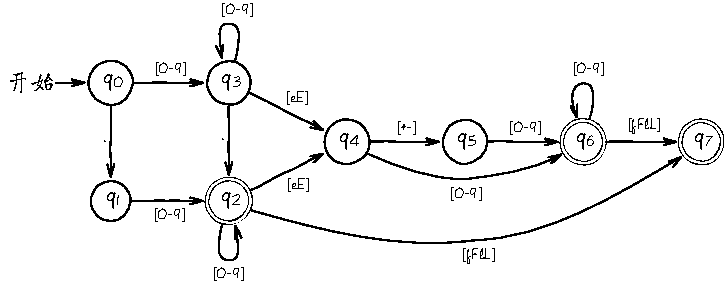
\includegraphics[scale=1.5]{automata_hand.pdf}
  \caption{严教授手画的有限自动机:它描述了 C 语言中浮点型字面值的词法。}
  \label{fig:automatahand}
\end{figure}

然而,尽管\autoref{fig:automatahand} 中严教授的自动机画得很仔细,但要在他的课
程幻灯片中使用,还是太粗疏了。严教授需要的是色彩鲜明、清晰准确的自动机图形,
就像\autoref{fig:automata} 中的一样。
\begin{figure}[htpb]
  \centering
  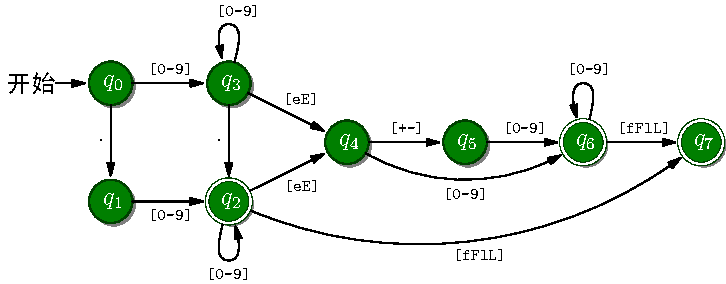
\includegraphics[scale=1.5]{automata.pdf}
  \caption{严教授想要在幻灯片里使用的有限自动机}
  \label{fig:automata}
\end{figure}

经过考虑,严教授决定用 \Asy{} 语言来完成这样的绘图,因为这样可以画出最精确的
图形,并能方便地对图形的所有细节进行控制,并且适合绘制大量形式相近的图形。然
而要让图形和生成图形的代码都接近完美,也将是一个艰巨的任务。

\section{标签和连线}
\label{sec:object}

把一些相似的小图形用线和箭头连接起来,是应用中非常广泛的一种作图类型。工作程
序的流程图、电路设计图、网络结构图、计算机科学中的自动机、乃至古老的家谱,都
可以看作是这类图形。这些相似的小图形往往是以一个文字标签为中心、用某种形状的
曲线围成的,再以各种线连接为一个整体——它可以抽象为数学中的“图”。这类图形
可以统称为图论图形,这正是计算机科学中使用最多的一类图形,也是严宇教授工作的
重点。

\Asy{} 语言已经提供了一种给标签围上边框,再连上线条的方法。这依赖于一种特殊的
数据类型:|object|(物件)。\index{object@\asyinline=object=}一个物件就是一个
带有某种形状边框的文字标签。函数
\index{draw@\asyinline=draw=}
\begin{asycode}
object draw(picture pic=currentpicture, Label L, envelope e,
            pair position=(0,0), real xmargin=0, real ymargin=xmargin,
            pen p=currentpen, filltype filltype=NoFill);
\end{asycode}
将在图 |pic| 上的位置 |position| 画出一个以标签 |L| 为中心,边框形状为 |e| 的
物件。参数 |xmargin| 和 |ymargin| 是边框与标签边沿的距离,画笔 |p| 用来绘制文
字标签,而 |filltype| 控制边框如何绘制和填充。
\index{filltype@\asyinline=filltype=}

\Asy{} 的这个函数初看起来非常复杂,但排除默认的参数,使用起来是直接了当的:
\begin{asycode}
object cat = draw("cat", box, (0,0), filltype=Draw),
       dog = draw("dog", ellipse, (2cm,0), filltype=Fill(olive)),
       elephant = draw("elephant", roundbox, (0,-2cm),
                       filltype=FillDraw(lightblue, darkblue));
\end{asycode}
\begin{figure}[H]
  \centering
\begin{asy}
object cat = draw("cat", box, (0,0), filltype=Draw),
       dog = draw("dog", ellipse, (2cm,0), filltype=Fill(olive)),
       elephant = draw("elephant", roundbox, (0,-2cm),
                       filltype=FillDraw(lightblue, darkblue));
\end{asy}
\end{figure}
\index{box@\asyinline=box=} \index{ellipse@\asyinline=ellipse=}
\index{roundbox@\asyinline=roundbox=} \index{Draw@\asyinline=Draw=}
\index{Fill@\asyinline=Fill=} \index{FillDraw@\asyinline=FillDraw=}
这里 |box|、|ellipse| 和 |roundbox| 分别是矩形、椭圆和圆角矩形三种可以使用的
形状;|Draw|、|Fill|、|FillDraw| 则分别是对边框画线、填充的控制变量(参考
\cite{asyman})。调用 |draw| 函数时如果省略 |filltype| 参数,则这里的默认值
|NoFill| 效果和 |Draw| 一样,表示使用画笔 |p| 绘制边框。

下面的问题则是把这些物件用线连接起来。为此,\Asy{} 提供了一种看起来颇为古怪的
方式:
\begin{asycode}
add(
    new void(picture pic, transform t) {
        draw(pic, point(cat,E,t) -- point(dog,W,t), Arrow);
        draw(pic, point(cat,S,t) -- point(elephant,N,t), Arrow);
        draw(pic, point(elephant,NE,t) -- point(dog,SW,t), Arrows);
        draw(pic, "curve", point(cat,SW,t) {SW} .. {SE} point(elephant,NW,t));
    }
);
\end{asycode}
\begin{figure}[H]
  \centering
\begin{asy}
object cat = draw("cat", box, (0,0), filltype=Draw),
       dog = draw("dog", ellipse, (2cm,0), filltype=Fill(olive)),
       elephant = draw("elephant", roundbox, (0,-2cm),
                       filltype=FillDraw(lightblue, darkblue));
add(
    new void(picture pic, transform t) {
        draw(pic, point(cat,E,t) -- point(dog,W,t), Arrow);
        draw(pic, point(cat,S,t) -- point(elephant,N,t), Arrow);
        draw(pic, point(elephant,NE,t) -- point(dog,SW,t), Arrows);
        draw(pic, "curve", point(cat,SW,t) {SW} .. {SE} point(elephant,NW,t));
    }
);
\end{asy}
\end{figure}
\index{add@\asyinline=add=}
在这里,实际只有一条语句 |add|,但 |add| 的参数则是一个匿名函数:
\index{函数!匿名函数}
\begin{asycode}
new void (picture pic, trasform t) {
    // `\color{comment}匿名函数体`
}
\end{asycode}
意思是在 |currentpicture|(|add| 省略的第一个参数)实际进行绘图时,就使用这个
匿名函数中的语句进行绘图\footnote{这种用法并没有在手册 \cite{asyman} 中描述,
它涉及 \asyinline=picture= 图类型内部的实现方式。这里添加的匿名函数就相当于添
加了一个等效的 \asyinline=drawer= 类型的函数。参看
\prgname{plain\_picture.asy} 中的代码。}。

上面匿名函数的内容就是画出 |cat|、|dog|、|elephant| 之间的连线,其中用到了有
关 |object| 物件类型的一个函数 |point|\footnote{函数 \asyinline=point= 也没有
在手册 \cite{asyman} 中描述。关于此函数以及预置的物件形状 \asyinline=box=、
\asyinline=roundbox= 和 \asyinline=ellipse= 的定义,参看
\prgname{plain\_boxes.asy} 中的代码。}:
\index{point@\asyinline=point=}
\begin{asycode}
pair point(object F, pair dir, transform t=identity());
\end{asycode}
这个函数输出物件 |F| 的边框在 |dir| 方向的坐标。这个坐标通过 |t| 作变换。注意
这里的方向 |dir| 是经过边框形状矫正过的,因而对于矩形物件,|NE| 方向的坐标点
就是矩形右上方向的直角点,而并非严格的 $45^\circ$ 角方向点。在匿名函数中,必
须把匿名函数的参数 |t| 传给函数 |point|,并且绘图时在参数 |pic| 的图中进行,
才能保证在正确的位置以正确的比例画出物件的坐标和连线。

在匿名函数中,只要注意正确地使用 |point| 函数和 |t|、|pic| 参数,对于绘图的语
句没有特别的限制。因此上面无论是连直线、曲线、箭头还是在连线上标注文字,都和
普通的方式一样。

尽管语法多少有些难看和冗繁,但使用 \Asy{} 中的物件类型和它的连线机制,就足够
画出各种形式的图论图形了。严教授的自动机也可以这样逐步构造出来。然而,严教授
最终却放弃了这种绘图的方式。不是因为这种方式的写法麻烦,而是因为这种方式很难
表达出一些有用的功能。例如,仅指定物件而不使用 |point| 函数指定具体连线的位置
来连接两个物件的能力,如在下面的代码中,我们能不能不去手工指定 |cat| 和 |dog|
的方向 |ENE| 和 |WSW| 呢?
\begin{asycode}
object cat = draw("cat", box, (0,0), filltype=Draw),
       dog = draw("dog", ellipse, (3cm,2cm), filltype=Fill(olive));
add(
    new void(picture pic, transform t) {
        draw(point(cat,ENE,t) -- point(dog,WSW,t));
    }
);
\end{asycode}
\begin{figure}[H]
  \centering
\begin{asy}
object cat = draw("cat", box, (0,0), filltype=Draw),
       dog = draw("dog", ellipse, (3cm,2cm), filltype=Fill(olive));
add(
    new void(picture pic, transform t) {
        draw(point(cat,ENE,t) -- point(dog,WSW,t));
    }
);
\end{asy}
\end{figure}
确实,如果是复杂的图论图形,靠人力算出连点合适的方向来,一不留神就会出错;而
如果想要通过一个循环自动化地连接五角星形呢?
\begin{figure}[H]
  \centering
\begin{asy}
import "figure-src/node.asy" as node;
real u = 1.5cm;
node[] p;
for (int i = 0; i < 5; ++i) {
    p[i] = Circle(string(i+1), u*dir(90+72i), drawer);
    draw(p[i]);
}
p.cyclic = true;
for (int i = 0; i < 5; ++i) {
    draw(p[i] -- p[i+2], Arrow);
    draw(p[i] .. bendright .. p[i+1], Arrow);
}
\end{asy}
\end{figure}
想要利用现有的 |object| 类型的连线机制画出上面的图形无疑就太麻烦了,因为定义
分布在正五边形上的五个物件或进行连线并不难(参看第\ref{chap:stars}章五角星的
画法),但要精确地确定五个圆形上连线的位置就非常令人头疼了。而严教授更希望他
能以一种更简单更自然的方式画连线,比如说:
\begin{asycode}
draw(cat -- dog);
\end{asycode}
如果真的可以这样做连线的话,那么要画出前面的五角星形就容易得多了。

不仅如此,还有一些工作是超出目前的 |object| 类型能力的。例如,产生 |object|
的 |draw| 函数只能支持 |box|、|ellipse| 和 |roundbox| 三种形状,而使用的
|filltype| 参数也只有 |FillDraw|、|Fill|、|Draw|、|NoFill|、|UnFill|、
|RadialShade|(参看 \cite{asyman})这么有限的几种。如果我们想要画出图形:
\begin{figure}[H]
  \centering
\begin{asy}
import "figure-src/node.asy" as node;
draw(Circle("A", (0,0), compose(shadow,filldrawer(yellow))));
draw(Circle("B", (2cm,0), white, ballshade));
\end{asy}
\end{figure}
那么我们就要增加新的圆形,新的带阴影的和带球形立体效果的 |filltype|——但在仔
细研究 \Asy{} 本身实现 |filltype| 和 |object| 相关类型的代码之前,我们甚至不
知道这种扩充能不能做到。在这种情况下,或者是通过研读 \Asy{} 中
\prgname{plain} 等基本模块(\Asy{} 在安装时就预定义好了许多模块,而其中最基本
的 \prgname{plain} 模块则会在运行时自动导入,我们平时使用的 \Asy{} 实际是建立
在 \prgname{plain} 模块之上的)的代码,自行扩充;或者需要自己重新实现一个新类
型。实际中很难说哪种方式更简单或更好用,但研究 \Asy{} 中 \prgname{plain} 模块
的实现,总是有教益的。

\section[解析代码与扩充功能]{解析代码与扩充功能\footnote{本节一些内容不易理解
,初次阅读时可跳过。}}
\label{sec:analyzecode}

下面我们就考虑上一节最后提出的一个简单问题:增加新的圆形 |envelope|。为此,我
们需要分析 \Asy{} 中 \prgname{plain} 模块的部分实现,然后对它进行扩充和修改。

在 \prgname{plain} 模块的一个子模块 \prgname{plain\_boxes.asy} 中,定义了有关
生成 |object| 类型的 |draw| 函数和 |box|、|roundbox|、|ellipse| 三种
|envelope| 类型的形状,|point| 函数的定义也在其中。如果我们需要新定义一种圆形
形状 |circle|,就可以模仿里面的代码。在研究相关的代码时,可能需要不断查阅手册
\cite{asyman}。

首先在 \prgname{plain\_boxes.asy} 的中间可以找到 |evelope| 类型的定义:
\index{envelope@\asyinline=envelope=}
\begin{asycode}
typedef path envelope(frame dest, frame src=dest, real xmargin=0,
                      real ymargin=xmargin, pen p=currentpen,
                      filltype filltype=NoFill, bool above=true);
\end{asycode}
这里使用了 |typedef| 命令定义类型的别名。\index{typedef@\asyinline=typedef=}
|typedef| 命令的用法是
\begin{asycode}
typedef `对标识符 foo 的声明`;
\end{asycode}
表示把 |foo| 定义为它所声明的类型的一个别名。如
\begin{asycode}
typedef int Integer;
\end{asycode}
就把 |Integer| 定义为整数类型 |int| 的别名,从而以后就可以用 |Integer| 来代替
|int|。上面就把 |envelope| 定义为一个函数类型的别名\footnote{但在 \Asy{} 中,
函数类型的别名只能用来声明一个函数变量,不能用于定义一个有函数体的函数。},这
个函数接受许多参数,而返回一条路径。不难猜想,这个函数返回的路径,正是将来生
成 |object| 类型元素的形状。

此时再看 \prgname{plain\_boxes.asy} 开头,就看到了 |box|、|roundbox| 和
|ellipse| 的定义,实际就是定义了三个函数。例如 |ellipse| 的定义(这里的代码来
自 \Asy{} 1.90 版本):
\begin{asycode}[numbers=left]
path ellipse(frame dest, frame src=dest, real xmargin=0, real ymargin=xmargin,
             pen p=currentpen, filltype filltype=NoFill, bool above=true)
{
  pair m=min(src);
  pair M=max(src);
  pair D=M-m;
  static real factor=0.5*sqrt(2);
  int sign=filltype == NoFill ? 1 : -1;
  path g=ellipse(0.5*(M+m),factor*D.x+0.5*sign*max(p).x+xmargin,
                 factor*D.y+0.5*sign*max(p).y+ymargin);
  frame F;
  if(above == false) {
    filltype.fill(F,g,p);
    prepend(dest,F);
  } else filltype.fill(dest,g,p);
  return g;
\end{asycode}
这个函数初看起来可能有点复杂。但如果只看它的返回值的话,那么函数主要的工作就
是返回路径 |g|,也就是 9、10 两行定义的椭圆。现在来分析函数的其他部分,4、5 
行定义的坐标 |m| 和 |M| 就是帧 |src| 的左下角和右下角点。其中帧\index{帧}
|frame|\index{frame@\asyinline=frame=} 是 \Asy{} 中类似于图 |picture| 的一种
功能更简单更基本的类型,不支持诸如自动放缩的功能;而函数
|min|\index{min@\asyinline=min=} 和 |max|\index{max@\asyinline=max=} 则接受帧
、图、路径甚至画笔(表示笔尖的路径)作为参数,分别返回它们的左下角和右上角的
坐标。于是,第 6 行定义的坐标 |D| 就是帧 |src| 的对角线向量。第 7 行定义了一
个静态(|static|\footnote{ 在这里表示一个常量,用静态类型保证只进行一次赋值。
有关静态类型请参看手册 \cite{asyman}。}\index{静态}
\index{static@\asyinline=static=})的实数因子 |factor| 为 $\sqrt{2}/2$。第 8
行判断填充类型 |filltype| 是否为空的 |NoFill| 而设置一个符号 |sign|。这样,9
、10 两行定义的椭圆就清楚了,它的中心就是帧 |src| 的中心,坐标为 $(M+m)/2$;
它的横轴半径是因子 |factor| 乘以对角线向量的横坐标 |D.x|,加上(或当
|filltype| 不为 |NoFill| 时减去)笔尖边框右上角位置的横坐标的一半\footnote{不
难发现其实这个实现是错误的,原来的代码试图给长轴加上笔尖宽度的一半,以保证即
使画笔很粗,也可以让边框线与标签内容间有正确的距离;由于笔尖的路径相对于原点
对称,这里计算笔尖边框右上角坐标的一半,其实只是笔尖宽度的 $1/4$。正确的实现
应该是 \asyinline{0.5*sign*(max(p)-min(p))}。在 1.91 以后版本的 \Asy{} 中,这
个错误已经修正。},
再加上用户定义的距离 |xmargin|;纵轴的定义与长轴类似。后面的 11
至 15 行,实际就是根据 |above| 的具体取值,对边框的填充和画线(|above| 为假时
在目标帧 |dest| 底部绘制)。

通过对比不难发现,|box| 与 |roundbox| 的实现与 |ellipse| 实际上大同小异。因此
我们很容易模仿它们写出圆形的 |envelope| 函数\footnote{修正了椭圆中计算轴长方
法中的小错误。}:
\begin{asycode}
// `\color{comment}circle 函数就是一个 envelope 类型的变量`
path circle(frame dest, frame src=dest, real xmargin=0, real ymargin=xmargin,
             pen p=currentpen, filltype filltype=NoFill, bool above=true)
{
    pair m=min(src);
    pair M=max(src);
    pair D=M-m;
    static real factor=0.5*sqrt(2);
    int sign=filltype == NoFill ? 1 : -1;
    // `\color{comment}圆的半径 r 就是前面定义中椭圆的横轴与纵轴中的较大值`
    real r = max(factor*D.x+sign*max(p).x+xmargin,
                 factor*D.y+sign*max(p).y+ymargin);
    path g=circle(0.5*(M+m), r);
    frame F;
    if(above == false) {
        filltype.fill(F,g,p);
        prepend(dest,F);
    } else filltype.fill(dest,g,p);
    return g;
}
\end{asycode}

把这段代码放在前面,马上就可以试验效果:
\begin{asycode}
object cat = draw("cat", circle, (0,0)),
       dog = draw("dog", circle, (2cm,0), filltype=Fill(olive));
add(
    new void(picture pic, transform t) {
        draw(point(cat,E,t) -- point(dog,W,t), Arrow);
    }
);
\end{asycode}
\begin{figure}[H]
  \centering
\begin{asy}
path circle(frame dest, frame src=dest, real xmargin=0, real ymargin=xmargin,
             pen p=currentpen, filltype filltype=NoFill, bool above=true)
{
    pair m=min(src);
    pair M=max(src);
    pair D=M-m;
    static real factor=0.5*sqrt(2);
    int sign=filltype == NoFill ? 1 : -1;
    real r = max(factor*D.x+sign*max(p).x+xmargin,
                 factor*D.y+sign*max(p).y+ymargin);
    path g=circle(0.5*(M+m), r);
    frame F;
    if(above == false) {
        filltype.fill(F,g,p);
        prepend(dest,F);
    } else filltype.fill(dest,g,p);
    return g;
}

object cat = draw("cat", circle, (0,0)),
       dog = draw("dog", circle, (2cm,0), filltype=Fill(olive));
add(
    new void(picture pic, transform t) {
        draw(point(cat,E,t) -- point(dog,W,t), Arrow);
    }
);
\end{asy}
\end{figure}

这样,通过分析并模仿 \prgname{plain} 模块原有的代码,就完成了一种新的
|envelope| 形状 |circle|,并能将其付诸使用。

但是,有关 |envelope| 类型的函数是比较复杂的,要想真正看懂它,像上面这样分析
清楚,甚至可能需要了解一些手册 \cite{asyman} 中没有提及的东西,也就是分析更多
的源代码。例如上面 |filltype| 的内部结构在手册中并没有给出说明,而需要分析
\prgname{plain\_filldraw.asy} 的代码;以画笔为参数的函数 |max| 也没有文档,更
需要到 \Asy{} 的 C++ 代码 \prgname{runtime.in} 和 \prgname{pen.h} 中才能找到
定义。

上面分析 |ellipse| 函数的过程可以看做一般的分析 \Asy{} 源代码的一个缩影。有时
所分析的代码比较简单,可以像上面那样比较容易地看清楚代码的来龙去脉,并对它进
行必要的扩充和修改;有时问题则会变得困难,需要缺少文档的情况下,在许多个源文
件中搜索需要的定义(比如由 |ellipse| 的定义查找 |filltype| 的内部结构和 |max|
函数在 \prgname{runtime.in} 中的定义)。并非人人像严教授这样是这方面的专家,
在很多情况下,分析源代码耗费的精力会比重写一遍相同功能的代码还要多,甚至会遇
到看不懂源代码的情形。这时,就必须要考虑解决问题的其他途径了。

\section{结构体与抽象机制}
\label{sec:struct}

出于对功能的扩充和最终用法简洁性的要求,严教授还是决定自己来设计一个新的类型
来完成他的自动机的绘制。

\Asy{} 中的数据类型是十分丰富的,除了整数(|int|)、实数(|real|)、坐标(
|pair|,即复数)、路向(|guide|)、路径(|path|)等基本类型,还有画笔(|pen|
)、图(|picture|)等预置的复杂类型,还有函数和数组类型。然而,更重要的是,
\Asy{} 还有把这些类型组合起来,建立新类型的一般方法,也就是对数据的抽象机制,
这就是结构体。\Asy{} 中的结构体与 C/C++ 语言的结构体在语法上十分接近,同时也
有自己的特点。\index{结构体}

一个结构体类型用下面的语法定义:
\index{struct@\asyinline=struct=}
\begin{asycode}
struct `结构体名` {
    `类型$_1$` `成员变量$_1$`;
    `类型$_2$` `成员变量$_2$`;
    `……`
}
\end{asycode}
这样,就把若干个类型的变量结合为一个整体,形成一个新的类型。例如,可以把两个
实数类型的变量复合为一种新的坐标类型:
\begin{asycode}
struct newpair {
    real x, y;
}
\end{asycode}
于是,就可以使用这种新的类型 |newpair| 来声明一个复合类型的变量,并且像普通
的 |pair| 类型一样,可以使用圆点运算符来分别得到它的两个分量:
\begin{asycode}
newpair a;     // `\color{comment}定义 newpair 类型的变量 a`
a.x = 1.0;      // `\color{comment}给 a 的 x 分量赋值`
a.y = 2.5;      // `\color{comment}给 a 的 y 分量赋值`
\end{asycode}
这样,就可以用一个变量名 |a| 表示相互紧密联系的两个量 |a.x| 和 |a.y|。这就是
数据的抽象。

物件类型 |object| 实际上就是把一个表示边框的路径和边框中的内容结合组成的结构
体\footnote{参看 \prgname{plain\_Label.asy} 的源代码。}。严教授需要的也就是与
|object| 类型的一个类似的类型,使用相同的方法,把一个边框路径、它的内容(用图
表示)以及它的位置结合为一个结构,并命名为“结点”|node|:
\begin{asycode}
// `\color{comment}结点类型,第一个实现`
struct node {
    path outline;   // `\color{comment}边框`
    picture stuff;  // `\color{comment}内容`
    pair pos;       // `\color{comment}位置`
}
\end{asycode}
于是,就可以写出这样的语句:
\begin{asycode}
node cat;                                   // `\color{comment}定义 cat 结点`
cat.outline = circle((0,0), 4mm);           // `\color{comment}cat 的边框是一个圆`
cat.pos = (0,0);                            // `\color{comment}cat 的位置在原点`
filldraw(cat.stuff, cat.outline, yellow);   // `\color{comment}把边框画进 cat 的内容`
label(cat.stuff, "cat");                    // `\color{comment}把文字标进 cat 的内容`
add(shift(cat.pos) * cat.stuff);            // `\color{comment}在指定位置画出 cat 的内容`
\end{asycode}
\begin{figure}[H]
  \centering
\begin{asy}
struct node {
    path outline;
    picture stuff;
    pair pos;
}
node cat;
label(cat.stuff, "cat");
cat.outline = circle((0,0), 4mm);
cat.pos = (0,0);
filldraw(cat.stuff, cat.outline, yellow);
add(cat.stuff);
\end{asy}
\end{figure}
这无疑是十分简陋的,还远远比不上 |object| 类型的精致。但这已经展示出了操作
|node| 类型的最重要的手段。下面要做的事就是,用函数把上面的一个个独立的操作包
装起来。

首先是使用函数建立一个 |node| 类型的变量,它的内容是一个文字标签,边框是紧密
围绕在标签之外的一个圆形,而位置由函数的参数指定。不仅如此,还要指定边框和标
签分别怎么在 |node| 的内容中画出来,最简单的办法就是分别指定一些画笔:
\begin{asycode}
// `\color{comment}圆形结点的构造函数,第一个实现`
node Circle(Label text, pair pos, pen textpen=currentpen,
            pen fillpen=nullpen, pen drawpen=currentpen)
{
    node nd;        // `\color{comment}定义新结点`
    nd.pos = pos;   // `\color{comment}设置位置`
    label(nd.stuff, text, textpen);             // `\color{comment}在内容中标注文字`
    pair M = max(nd.stuff), m = min(nd.stuff);  // `\color{comment}计算内容边界大小`
    nd.outline = circle(0.5*(M+m), 0.5*length(M-m));    // `\color{comment}设置边框`
    filldraw(nd.stuff, nd.outline, fillpen, drawpen);   // `\color{comment}绘制和填充边框`
    return nd;      // `\color{comment}返回构造的新结点`
}
\end{asycode}
这里计算内容边界并设置圆形边框路径的办法,就是前面为 |object| 类型建立圆形
|envelope| 的算法的特别简化的版本:计算出左下、右上角的坐标,得到中心坐标和对
角线长度,就是边框的圆心和直径。

然后是定义一个函数画出整个结点,方法和单独把结点的内容加进当前图一样:
\begin{asycode}
// `\color{comment}画结点,简单实现`
void draw(picture pic=currentpicture, node nd)
{
    add(pic, shift(nd.pos) * nd.stuff);
}
\end{asycode}

于是,利用上面的函数,就可以这样来画出结点了:
\begin{asycode}
node cat = Circle("cat", (0,0), fillpen=yellow),
     dog = Circle("dog", (2cm,0), fillpen=olive, drawpen=nullpen);
draw(cat);
draw(dog);
\end{asycode}
\begin{figure}[H]
  \centering
\begin{asy}
struct node {
    path outline;
    picture stuff;
    pair pos;
}
node Circle(Label text, pair pos, pen textpen=currentpen,
            pen fillpen=nullpen, pen drawpen=currentpen)
{
    node nd;
    nd.pos = pos;
    label(nd.stuff, text, textpen);
    pair M = max(nd.stuff), m = min(nd.stuff);
    nd.outline = circle(0.5*(M+m), 0.5*length(M-m));
    filldraw(nd.stuff, nd.outline, fillpen, drawpen);
    return nd;
}
void draw(picture pic=currentpicture, node nd)
{
    add(pic, shift(nd.pos) * nd.stuff);
}
node cat = Circle("cat", (0,0), fillpen=yellow),
     dog = Circle("dog", (2cm,0), fillpen=olive, drawpen=nullpen);
draw(cat);
draw(dog);
\end{asy}
\end{figure}

现在来看怎么实现 |object| 类型中 |point| 函数的对应物。类似 |point(cat,E,t)|
的用法无疑是太蹩脚了,比如理想的方式是 |cat.E|。按前面 |node| 类型的定义,只
要给 |node| 增加一组变量,分别保存边框在不同方向上的点的坐标。但更一般地,直
接得到边框在某个特定方向(或角度)上的点也是非常有用的,因此最好还有一种类似
|point.angle(30)| 或 |point.dir(ENE)| 的语法,来表示边框上的特定方向的点。对
此,也只要在结构体 |node| 中增加几个函数类型作为成员。因此,可以这样扩充
|node| 类型:
\begin{asycode}
// `\color{comment}结点类型,第二个实现`
struct node {
    path outline;
    picture stuff;
    pair pos;
    pair E, N, W, S;
    pair dir(pair v)
    {
        path g = shift(pos) * outline;
        pair M = max(g), m = min(g), c = 0.5*(M+m);
        path ray = c -- c + length(M-m)*unit(v);
        return intersectionpoint(g, ray);
    }
    pair angle(real ang)
    {
        return this.dir(dir(ang));
    }
}
\end{asycode}

这里需要解释的函数是新加进来的 |dir| 函数。就像上面做的,在结构体中可以直接定
义函数,即这个结构体的成员函数\index{成员函数}\index{结构体!成员函数}。在
\Asy{} 中,成员函数也是结构体的普通成员变量,结构体里面的函数定义只是给了这个
变量一个初始值。在 |dir| 函数中,它接受一个表示方向的坐标变量 |v|,返回从结点
边框的中心发出的在 |v| 方向的射线与边框路径的交点,也就是我们要的边框在 |v| 
方向上的点。|dir| 函数的计算过程是简单而清晰的:首先通过平移得到正确的边框路
径 |g|,而后计算边框的右上角坐标 |M|、左下角坐标 |m|、中心坐标 |c|,而后计算
射线 |ray|,最后返回交点坐标。其中用到的 |length|
\index{length@\asyinline=length=} 函数计算向量的长度(也就是对应复数的绝对值
),|unit|\index{unit@\asyinline=unit=} 函数计算与向量方向相同的单位向量,而
|intersectionpoint| 正是 \autoref{sec:guide2path} 中的求两路径交点的函数。在
成员函数 |dir| 中,可以直接使用结构体里面定义的变量,而不必再通过参数传递,这
正是结构体成员函数的方便之处。

另一个成员函数 |angle| 只是简单地调用刚刚定义的 |dir| 函数,完成类似的功能。
不过这里的语句有点令人疑惑:前面对 |dir| 的定义实际是重载了 \Asy{} 本来就有一
个函数 |dir|,因而 |angle| 要使用两个 |dir| 函数,一个是成员函数 |dir(pair)| 
计算交点,另一个是系统的 |dir(real)| 计算一个角度方向上的向量。正像前面
\autoref{sec:randomarray} 中所说的,重载的两个函数参数类型不同,所以可以直接
用 |dir(dir(ang))|,并不会产生歧义,但为了避免读代码的人混淆,这里用了
|this.dir| 来表示结构体的成员函数。|this|\index{this@\asyinline=this=} 是一个
特殊的关键字,可以用来代替这个结构体类型的实例本身(如已经定义了 |node| 类型
的变量 |a|,那么调用 |a.angle(0)| 时,|a.angle| 函数中的 |this| 就代表 |a| 本
身,从而 |this.dir| 就是 |a.dir|)。

此时,结点类型 |node| 增加了 |E|、|N|、|W|、|S| 几个坐标用来方便地访问边框上
的点,这些坐标也必须在用函数构造结点类型时就进行初始化。这就需要在 |Circle| 
函数中增加几个语句,调用成员函数 |dir| 函数完成这个工作:
\begin{asycode}
// `\color{comment}圆形结点的构造函数,第二个实现`
node Circle(Label text, pair pos, pen textpen=currentpen,
            pen fillpen=nullpen, pen drawpen=currentpen)
{
    node nd;
    nd.pos = pos;
    label(nd.stuff, text, textpen);
    pair M = max(nd.stuff), m = min(nd.stuff);
    nd.outline = circle(0.5*(M+m), 0.5*length(M-m));
    filldraw(nd.stuff, nd.outline, fillpen, drawpen);
    nd.E = nd.dir(E);   // `\color{comment}调用 nd.dir 函数对四个方向初始化`
    nd.N = nd.dir(N);
    nd.W = nd.dir(W);
    nd.S = nd.dir(S);
    return nd;
}
\end{asycode}

对结点类型的 |draw| 函数不需要做改变。因此,下面就不仅可以画出结点,而且可以
像使用原来的 |object| 类型一样,画出连线了:
\begin{asycode}
node cat = Circle("cat", (0,0), fillpen=yellow),
     dog = Circle("dog", (2cm,0), fillpen=olive, drawpen=nullpen);
draw(cat);
draw(dog);
draw(cat.E -- dog.W, Arrow);
// `\color{comment}等价地,也可以用`
// draw(cat.dir(E) -- cat.dir(W), Arrow);
// `\color{comment}或者`
// draw(cat.angle(0) -- cat.angle(180), Arrow);
\end{asycode}
\begin{figure}[H]
  \centering
\begin{asy}
// `\color{comment}结点类型,第二个实现`
struct node {
    path outline;
    picture stuff;
    pair pos;
    pair E, N, W, S;
    pair dir(pair v)
    {
        path g = shift(pos) * outline;
        pair M = max(g), m = min(g), c = 0.5*(M+m);
        path ray = c -- c + length(M-m)*unit(v);
        return intersectionpoint(g, ray);
    }
    pair angle(real ang)
    {
        return this.dir(dir(ang));
    }
}

// `\color{comment}圆形结点的构造函数,第二个实现`
node Circle(Label text, pair pos, pen textpen=currentpen,
            pen fillpen=nullpen, pen drawpen=currentpen)
{
    node nd;
    nd.pos = pos;
    label(nd.stuff, text, textpen);
    pair M = max(nd.stuff), m = min(nd.stuff);
    nd.outline = circle(0.5*(M+m), 0.5*length(M-m));
    filldraw(nd.stuff, nd.outline, fillpen, drawpen);
    nd.E = nd.dir(E);
    nd.N = nd.dir(N);
    nd.W = nd.dir(W);
    nd.S = nd.dir(S);
    return nd;
}

void draw(picture pic=currentpicture, node nd)
{
    add(pic, shift(nd.pos) * nd.stuff);
}

node cat = Circle("cat", (0,0), fillpen=yellow),
     dog = Circle("dog", (2cm,0), fillpen=olive, drawpen=nullpen);
draw(cat);
draw(dog);
draw(cat.E -- dog.W, Arrow);
// `\color{comment}等价地,也可以用`
// draw(cat.dir(E) -- cat.dir(W), Arrow);
// `\color{comment}或者`
// draw(cat.angle(0) -- cat.angle(180), Arrow);
\end{asy}
\end{figure}

现在,利用结构体进行数据抽象,定义函数对抽象数据类型进行操作,我们就已经完成
了对原来 \Asy{} 中预定义的 |object| 类型一个简单的模拟。在这个过程中,我们失
去了一些功能:新的 |node| 类型不能使用 |size| 函数正确地进行放缩,因为它并不
像 |object| 类型在绘制时还小心冀冀地处理一个变换 |t|(见
\autoref{sec:object});也没有像原来的 |object| 类型那样在计算边框线粗细等细
节上锱铢必较(见 \autoref{sec:analyzecode})。但也得到了许多好处,那就是使用
时的简洁、清晰和容易修改扩充。而要完成这些,只要二三十行的代码。对比代码
\begin{asycode}
draw(cat.E -- dog.W);
\end{asycode}
和
\begin{asycode}
add(
    new void(picture pic, transform t) {
        draw(point(cat,E,t) -- point(cat,W,t));
    }
;)
\end{asycode}
其实不难做出抉择。

\section{运算符和记法}
\label{sec:operator}

然而,严教授并不满足于让 |node| 重复 |object| 类型的功能,他需要的是更简单、
更有效的写法:
\begin{asycode}
draw(cat -- dog);
\end{asycode}
尽管看上去差别不大,但从 |cat.E| 到 |cat| 的转变是本质性的,这个区别比从
|point(cat,E,t)| 到 |cat.E| 的区别还要大。因为无论是 |point(cat,E,t)| 还是
|cat.E|,都是一个 |pair| 类型的量,用它来连线是顺理成章的;但 |cat| 则是
|node| 类型的变量,两个 |node| 类型的变量用 |--| 连起来是什么东西?它们又怎么
能连起来呢?

这就引发了一个新的问题,就是发明一种把两个 |node| 类型连接起来的新的记法。而
这个语法是本来在 \Asy{} 中是没有的。要完成这一点,就需要使用运算符的重载。
\index{运算符重载}\index{重载!运算符重载}

在 \Asy{} 中,像 |+|、|-|、|*|、|/| 以及 |--|、|..| 这些运算符,都可以看成是
一个以 |operator|\index{operator@\asyinline=operator=} 开头的函数
\footnote{在 \Asy{} 中,绝大部分运算符都可以看做是函数,从而可以重载,甚至包
括一些在基本语言中没有的运算符,如 \asyinline=@=。但也有一些例外,包括赋值、
圆点、中括号(下标)、圆括号(函数调用)和条件运算符。}。如整数的加法运算符
|+| 就等价于函数
\begin{asycode}
int operator+(int op1, int op2);
\end{asycode}
它接受两个整数参数,返回它们的和。因而 |1+2| 就等价于 |operator+(1,2)|,都得
到结果 |3|。

既然运算符就是函数,那么就可以自己定义;即使已经有了定义,按照
\autoref{sec:randomarray} 中所说,也可以自己重载。因而,完全可以通过重载,定
义一种不寻常的整数加法:
\begin{asycode}
// `\color{comment}保存旧的加法定义`
int oldadd(int op1, int op2) = operator+;
// `\color{comment}定义新的加法为模 5 意义下的加法`
int operator+(int op1, int op2)
{
    return oldadd(op1, op2) % 5;
}
\end{asycode}
也就是把加号 |+| 定义为 $\mathbb{Z}_5$ 上的加法运算了。那么 |1+2| 的结果仍然
是 |3|,但 |2+3| 的结果就成了 |0|,|2+4| 则得到 |1|。

这样,利用自定义运算符 |--|,严教授就顺理成章地完成了两个结点之间的连线定义:
\begin{asycode}
path operator--(node nd1, node nd2)
{
    path g1 = shift(nd1.pos) * nd1.outline;
    path g2 = shift(nd2.pos) * nd2.outline;
    pair c1 = (max(g1)+min(g1)) / 2;
    pair c2 = (max(g2)+min(g2)) / 2;
    path edge = c1 -- c2;
    edge = firstcut(edge, g1).after;
    edge = lastcut(edge, g2).before;
    return edge;
}
\end{asycode}
这里,|operator--| 函数接受两个结点参数。它首先计算两个结点的边框路径 |g1| 和
|g2|,然后算出两个边框的中心 |c1| 和 |c2|,然后定义结点的连线 |edge| 就是
|c1 -- c2|,最后利用 |firstcut| 和 |lastcut| 函数截取 |edge| 在 |g1| 交点后面
、在 |g2| 交点前面的中间一段,就是正确的连线。
\index{firstcut@\asyinline=firstcut=}
\index{lastcut@\asyinline=lastcut=}

在这里,函数 |firstcut| 和 |lastcut| 分别是函数 |cut|
\index{cut@\asyinline=cut=} 的在 |n| 为 |0| 和 |-1| 时的特例:
\begin{asycode}
slice cut(path p, path knife, int n);
\end{asycode}
|cut| 函数返回一个结构体 |slice|\index{slice@\asyinline=slice=}:
\index{before@\asyinline=before=}
\index{after@\asyinline=after=}
\begin{asycode}
struct slice {
    path before,after;
}
\end{asycode}
它计算路径 |p| 与 |knife| 的第 |n| 个(负数表示倒数)交点,把 |p| 分成两半:
其中 |before| 是把路径 |p| 用“刀” |knife| 切开的前半截,而 |after| 是后半截
。

好了,现在严教授就可以这样画出两个结点及连线了:
\begin{asycode}
node cat = Circle("cat", (0,0), fillpen=yellow),
     dog = Circle("dog", (2cm,0), fillpen=olive, drawpen=nullpen);
draw(cat);
draw(dog);
draw(cat -- dog, Arrow);
\end{asycode}
\begin{figure}[H]
  \centering
\begin{asy}
// `\color{comment}结点类型,第二个实现`
struct node {
    path outline;
    picture stuff;
    pair pos;
    pair E, N, W, S;
    pair dir(pair v)
    {
        path g = shift(pos) * outline;
        pair M = max(g), m = min(g), c = 0.5*(M+m);
        path ray = c -- c + length(M-m)*unit(v);
        return intersectionpoint(g, ray);
    }
    pair angle(real ang)
    {
        return this.dir(dir(ang));
    }
}

// `\color{comment}圆形结点的构造函数,第二个实现`
node Circle(Label text, pair pos, pen textpen=currentpen,
            pen fillpen=nullpen, pen drawpen=currentpen)
{
    node nd;
    nd.pos = pos;
    label(nd.stuff, text, textpen);
    pair M = max(nd.stuff), m = min(nd.stuff);
    nd.outline = circle(0.5*(M+m), 0.5*length(M-m));
    filldraw(nd.stuff, nd.outline, fillpen, drawpen);
    nd.E = nd.dir(E);
    nd.N = nd.dir(N);
    nd.W = nd.dir(W);
    nd.S = nd.dir(S);
    return nd;
}

void draw(picture pic=currentpicture, node nd)
{
    add(pic, shift(nd.pos) * nd.stuff);
}

path operator--(node nd1, node nd2)
{
    path g1 = shift(nd1.pos) * nd1.outline;
    path g2 = shift(nd2.pos) * nd2.outline;
    pair c1 = (max(g1)+min(g1)) / 2;
    pair c2 = (max(g2)+min(g2)) / 2;
    path edge = c1 -- c2;
    edge = firstcut(edge, g1).after;
    edge = lastcut(edge, g2).before;
    return edge;
}

node cat = Circle("cat", (0,0), fillpen=yellow),
     dog = Circle("dog", (2cm,0), fillpen=olive, drawpen=nullpen);
draw(cat);
draw(dog);
draw(cat -- dog, Arrow);
\end{asy}
\end{figure}

事情还没有完。上面只是定义了两个结点之间的直线连接,严教授还需要用曲线把结点
连接起来。也就是说,严教授还希望有某种方便的 |..| 运算符。

理想中的 |..| 运算符应该是什么样的?回想第\ref{chap:tiling}章中曲线的绘制。把
两个结点直接用 |..| 连起来是没有什么用的,因为 |cat..dog| 就应该得到一条直线
,那么 |cat--dog| 就足够了;而 |cat{NE}..{SE}dog| 这种记法合理一些,但也好不
到哪里去,因为它并不比 |cat.dir(NE){NE}..{SE}dog.dir(SW)| 简单多少,同样需要
手工去设想准确的连接方向。至于 |tension|、|curl| 等,更难看出实际的用处来。
——说到底,严教授需要的是一种完全不同于以往的记法。考虑这个图形:
\begin{asycode}
node cat = Circle("cat", (0,0), fillpen=yellow),
     dog = Circle("dog", (5cm,0), fillpen=olive, drawpen=nullpen);
draw(cat);
draw(dog);
draw(cat.angle(30){dir(30)} .. {dir(-30)}dog.angle(150), Arrow);
\end{asycode}
\begin{figure}[H]
  \centering
\begin{asy}
// `\color{comment}结点类型,第二个实现`
struct node {
    path outline;
    picture stuff;
    pair pos;
    pair E, N, W, S;
    pair dir(pair v)
    {
        path g = shift(pos) * outline;
        pair M = max(g), m = min(g), c = 0.5*(M+m);
        path ray = c -- c + length(M-m)*unit(v);
        return intersectionpoint(g, ray);
    }
    pair angle(real ang)
    {
        return this.dir(dir(ang));
    }
}

// `\color{comment}圆形结点的构造函数,第二个实现`
node Circle(Label text, pair pos, pen textpen=currentpen,
            pen fillpen=nullpen, pen drawpen=currentpen)
{
    node nd;
    nd.pos = pos;
    label(nd.stuff, text, textpen);
    pair M = max(nd.stuff), m = min(nd.stuff);
    nd.outline = circle(0.5*(M+m), 0.5*length(M-m));
    filldraw(nd.stuff, nd.outline, fillpen, drawpen);
    nd.E = nd.dir(E);
    nd.N = nd.dir(N);
    nd.W = nd.dir(W);
    nd.S = nd.dir(S);
    return nd;
}

void draw(picture pic=currentpicture, node nd)
{
    add(pic, shift(nd.pos) * nd.stuff);
}

path operator--(node nd1, node nd2)
{
    path g1 = shift(nd1.pos) * nd1.outline;
    path g2 = shift(nd2.pos) * nd2.outline;
    pair c1 = (max(g1)+min(g1)) / 2;
    pair c2 = (max(g2)+min(g2)) / 2;
    path edge = c1 -- c2;
    edge = firstcut(edge, g1).after;
    edge = lastcut(edge, g2).before;
    return edge;
}

node cat = Circle("cat", (0,0), fillpen=yellow),
     dog = Circle("dog", (5cm,0), fillpen=olive, drawpen=nullpen);
draw(cat);
draw(dog);
draw(cat.angle(30){dir(30)} .. {dir(-30)}dog.angle(150), Arrow);
\end{asy}
\end{figure}
最后一行的曲线连线看起来十分复杂,出现了四个角度,但它们其实加起来只表示一个
意思:就是从 |cat| 从左边偏 $30^\circ$ 连一条曲线拐到 |dog|,这个 $30^\circ$
是相对 |cat| 和 |dog| 的直线连线而说的。因此,看起来合情合理的记法就呼之欲出
了,它可以是这个样子的:
\begin{asycode}
draw(cat .. bendleft .. dog, Arrow);
\end{asycode}
这个记法很像是定义路向控制点的 |z0 .. controls c .. z1| 记法,因而也很容易理
解。而前面利用 |angle| 成员函数对 |cat| 和 |dog| 连线的复杂的写法,实际上揭示
了这个记法的实现方法。

如果不考虑新记法的问题,首先可以实现把两个结点用曲线连起来的一个函数。不妨就
叫它 |bendleft|:
\begin{asycode}
// `\color{comment}用弯曲路径连接两个结点,第一个实现`
path bendleft(node nd1, node nd2)
{
    path g1 = shift(nd1.pos) * nd1.outline;
    path g2 = shift(nd2.pos) * nd2.outline;
    pair c1 = (max(g1)+min(g1)) / 2;
    pair c2 = (max(g2)+min(g2)) / 2;
    real deg = degrees(c2 - c1);
    return nd1.angle(deg+30) {dir(deg+30)}
        .. {dir(deg-30)} nd2.angle(180+deg-30);
}
\end{asycode}
前面的计算就和直线连接一样,找出了两个结点的中心坐标 |c1| 和 |c2|。最后利用
|degrees| 函数(它计算向量的角度,正是 |dir| 函数的反函数),计算了直线
|c1--c2| 的角度 |deg|。最后返回的曲线路径就和前面直接连接 |cat| 和 |dog| 的过
程差不多,只是考虑了 |deg| 的影响:所谓向左偏 $30^\circ$,其实就是在角度
|deg| 的基础上加上 $30^\circ$,从而得到 |nd1| 边框上点的角度和在这点的曲线切
线方向,类似地可以得到 |nd2| 相关的角度。

要得到 |nd1 .. bendleft .. nd2| 这种新的记法,那大概就应该是一个接受三个参数
的运算符函数:
\begingroup
\renewcommand\thelstnumber{?}
\begin{asycode}[numbers=left]
typedef path edgeconnector(node nd1, node nd2);

path operator..(node nd1, edgeconnector con, node nd2)
{
    return con(nd1, nd2);
}
\end{asycode}
\endgroup
这里利用 |typedef| 定义了一个连线的 |edgeconnector| 类型,其实就是从两个结点
连成一条路径的函数类型的别名。然后就让 |operator..| 函数接受两个结点和一个连
线函数,返回用这个函数计算得到的连线。

可惜,当我们用 |cat .. bendleft .. dog| 来测试这段代码的使用时,\Asy{} 毫不留
情地发出了一条错误信息:
\begin{asycode}
`no matching function` 'operator ..(node, path(node nd1, node nd2))'
\end{asycode}
分析这条错误信息我们发现,\Asy{} 并不把 |cat .. bendleft .. dog| 看成是一个整
体,而是先按从左到右的优先级,去计算 |cat .. bendleft|,然后发现没有这种运算
符的定义的错误。这无疑是说,想要用一个 |operator..| 函数授受三个不同的参数的
做法是成功不了的,前面的定义是错误的。

看上去问题陷入了僵局:我们已经定义了十分方便的 |cat -- dog|,却无法正确定义
|cat .. bendleft .. dog|,而不得不使用 |bendleft(cat, dog)|。后一种函数调用的
记法并不复杂,但缺乏一致性。

然而严教授总有办法:既然 \Asy{} 只允许 |cat .. bendleft|,那么何不就让它先算
出一个正确的 |cat .. bendleft| 呢?可以让 |cat .. bendleft| 先算出一个中间值
(比如说 |f|),它包含 |cat| 和 |bendleft| 的全部信息,然后再计算 |f .. dog|
以 |bendleft(cat,dog)| 作为结果。这个过程有点技巧性,关键是需要一个中间值,它
仍然得是一个新的类型。

有两种实现中间值的办法,一种是使用结构体,一种是建立一个一元函数。严教授选择
了后一种,因为它更简洁,也更能体现函数作为一种动态数据的作用:
\begin{asycode}
typedef path edgeconnector(node nd1, node nd2);
typedef path edgemaker(node nd);

// `\color{comment}nd1 .. con .. nd2 的前一半`
edgemaker operator..(node nd, edgeconnector con)
{
    return new path(node nd2) {
        return con(nd, nd2);
    };
}

// `\color{comment}nd1 .. con .. nd2 的后一半`
path operator..(edgemaker maker, node nd)
{
    return maker(nd);
}
\end{asycode}
这时,使用
\begin{asycode}
draw(cat .. bendleft .. dog, Arrow);
\end{asycode}
就能画出正确的图形了。注意,严教授在函数 |operator..(node,edgeconnector)| 中
直接返回了一个新的函数,也就是一个 |edgemaker| 的对象。
\index{函数!作为返回值}

类似地,还可以定义右弯的函数 |bendright|,这和 |bendleft| 函数的区别仅仅在于
$30^\circ$ 的符号。不过严教授使用了更一般的方式定义了一个向任意角度弯转的
|bend| 函数:
\begin{asycode}
// `\color{comment}用弯曲路径连接两个结点,第二个实现`
edgeconnector bend(real ang)
{
    return new path (node nd1, node nd2) {
        path g1 = shift(nd1.pos) * nd1.outline;
        path g2 = shift(nd2.pos) * nd2.outline;
        pair c1 = (max(g1)+min(g1)) / 2;
        pair c2 = (max(g2)+min(g2)) / 2;
        real deg = degrees(c2 - c1);
        return nd1.angle(deg+ang) {dir(deg+ang)}
            .. {dir(deg-ang)} nd2.angle(180+deg-ang);
    };
}

edgeconnector bendleft = bend(30);
edgeconnector bendright = bend(-30);
\end{asycode}
这里,|edgeconnector| 类型的函数被作为 |bend| 的返回值得到,因而 |bendleft| 
就被定义为 |bend(30)|,而 |bendright| 被定义为 |bend(-30)|。如果需要更多的东
西,甚至还可以加上构造曲线的 |tension| 值,扩充的余地还有很大。

更进一步,严教授还需要给他的自动机画循环的函数,来画出这样的图形来:
\begin{figure}[H]
  \centering
\begin{asy}
// `\color{comment}结点类型,第二个实现`
struct node {
    path outline;
    picture stuff;
    pair pos;
    pair E, N, W, S;
    pair dir(pair v)
    {
        path g = shift(pos) * outline;
        pair M = max(g), m = min(g), c = 0.5*(M+m);
        path ray = c -- c + length(M-m)*unit(v);
        return intersectionpoint(g, ray);
    }
    pair angle(real ang)
    {
        return this.dir(dir(ang));
    }
}

// `\color{comment}圆形结点的构造函数,第二个实现`
node Circle(Label text, pair pos, pen textpen=currentpen,
            pen fillpen=nullpen, pen drawpen=currentpen)
{
    node nd;
    nd.pos = pos;
    label(nd.stuff, text, textpen);
    pair M = max(nd.stuff), m = min(nd.stuff);
    nd.outline = circle(0.5*(M+m), 0.5*length(M-m));
    filldraw(nd.stuff, nd.outline, fillpen, drawpen);
    nd.E = nd.dir(E);
    nd.N = nd.dir(N);
    nd.W = nd.dir(W);
    nd.S = nd.dir(S);
    return nd;
}

void draw(picture pic=currentpicture, node nd)
{
    add(pic, shift(nd.pos) * nd.stuff);
}

path operator--(node nd1, node nd2)
{
    path g1 = shift(nd1.pos) * nd1.outline;
    path g2 = shift(nd2.pos) * nd2.outline;
    pair c1 = (max(g1)+min(g1)) / 2;
    pair c2 = (max(g2)+min(g2)) / 2;
    path edge = c1 -- c2;
    edge = firstcut(edge, g1).after;
    edge = lastcut(edge, g2).before;
    return edge;
}

typedef path edgeconnector(node nd1, node nd2);
typedef path edgemaker(node nd);

// `\color{comment}nd1 .. con .. nd2 的前一半`
edgemaker operator..(node nd, edgeconnector con)
{
    return new path(node nd2) {
        return con(nd, nd2);
    };
}

// `\color{comment}nd1 .. con .. nd2 的后一半`
path operator..(edgemaker maker, node nd)
{
    return maker(nd);
}

edgeconnector bend(real ang)
{
    return new path (node nd1, node nd2) {
        path g1 = shift(nd1.pos) * nd1.outline;
        path g2 = shift(nd2.pos) * nd2.outline;
        pair c1 = (max(g1)+min(g1)) / 2;
        pair c2 = (max(g2)+min(g2)) / 2;
        real deg = degrees(c2 - c1);
        return nd1.angle(deg+ang) {dir(deg+ang)}
            .. {dir(deg-ang)} nd2.angle(180+deg-ang);
    };
}

edgeconnector bendleft = bend(30);
edgeconnector bendright = bend(-30);

path operator..(node nd, edgemaker maker)
{
    return maker(nd);
}

// `\color{comment}自动机循环`
edgemaker loop(pair direction, real ratio=1.5)
{
    return new path(node nd) {
        real deg = degrees(direction);
        real angle1 = deg - 15, angle2 = deg + 15;
        pair mid = nd.angle(deg)
            + ratio*fontsize(currentpen)*unit(direction);
        return nd.angle(angle1) {dir(angle1)} .. mid
            .. {-dir(angle2)} nd.angle(angle2);
    };
}

node cat = Circle("cat", (0,0), fillpen=yellow);
draw(cat);
draw(cat .. loop(up), Arrow);
\end{asy}
\end{figure}
现在只要对 |cat| 一个结点向自己做连线,怎样的记法才是最自然的呢?直接用函数的
形式 |loop(cat)| 就不错,如果需要确定循环连线的方向,那么 |loop(cat,up)| 也不
错。不过严教授坚持在连线时使用统一的记法,那么比较好的写法就应该是
\begin{asycode}
draw(cat .. loop(up), Arrow);
\end{asycode}

有了前面的东西,这个循环的记法并不难实现。而且严教授在前面定义的 |edgemaker|
类型在这里得到了应用:
\begin{asycode}
path operator..(node nd, edgemaker maker)
{
    return maker(nd);
}

// `\color{comment}自动机循环`
edgemaker loop(pair direction, real ratio=1.5)
{
    return new path(node nd) {
        real deg = degrees(direction);
        real angle1 = deg - 15, angle2 = deg + 15;
        pair mid = nd.angle(deg)
            + ratio*fontsize(currentpen)*unit(direction);
        return nd.angle(angle1) {dir(angle1)} .. mid
            .. {-dir(angle2)} nd.angle(angle2);
    };
}
\end{asycode}

最后,严教授发现,像 \autoref{sec:struct} 中那样每画一个结点就用一个 |draw| 
函数的方法也不是什么好的记法。理想的办法应该是可以在一个 |draw| 函数中使用任
意多个结点,就像
\begin{asycode}
draw(cat, dog, elephant);
\end{asycode}
这种方式。然而,要使用“任意多个”参数,就必须依赖 \Asy{} 的一种新的语法了,
那就是可变长参数表。

\index{可变长参数}\index{函数!可变长参数}
带有可变长参数的函数原型为:
\begin{asycode}
`返回类型` function(`前面的参数` ... T[] `数组`)
\end{asycode}
其中使用 |...| 把前面的参数和最后的一个数组类型的参数分开(中间没有逗号),前
面的参数和普通的函数参数一样,最后一个数组由在函数参数列表的末尾所有类型为
|T| 的那些参数构成。因为这些参数放在函数参数表的最后,所以在 \Asy{} 中又被称
为剩余参数(rest arguments)。\index{剩余参数}\index{函数!剩余参数}

因而,如果画出一个结点数组的函数是
\begin{asycode}
// `\color{comment}画出结点数组`
void draw(picture pic=currentpicture, node[] nodearr)
{
    for (node nd: nodearr)
        add(pic, shift(nd.pos) * nd.stuff);
}
\end{asycode}
则画出一次多个结点的函数就是
\begin{asycode}
// `\color{comment}画出一个或多个结点`
void draw(picture pic=currentpicture ... node[] nodearr)
{
    draw(pic, nodearr);
}
\end{asycode}
在 |draw| 的代码中,严教授又使用了一种新的 |for| 循环记法:
\index{for@\asyinline=for=}
\begin{asycode}
for (elem : arr)
    `循环语句体`
\end{asycode}
表示让 |elem| 取遍数组 |arr| 中的元素进行循环。

最终,把所有这些东西都用在一起,就足够用相当简洁的语法画出一个完整的自动机的
图形了(\autoref{fig:automatapreliminary}):
\begin{asycode}
real u = 2cm;
pen StateText = white;
pen StateFill = deepgreen;
pen StateDraw = darkgreen+0.6;
pen AcceptDraw = darkgreen+1.8;
node q0 = Circle("$q_0$", (0,0), StateText, StateFill, StateDraw),
     q1 = Circle("$q_1$", q0.pos + u*S, StateText, StateFill, StateDraw),
     q2 = Circle("$q_2$", q1.pos + u*E, StateText, StateFill, AcceptDraw),
     q3 = Circle("$q_3$", q0.pos + u*E, StateText, StateFill, StateDraw),
     q4 = Circle("$q_4$", q3.pos + u*E + 0.5u*S, StateText, StateFill, StateDraw),
     q5 = Circle("$q_5$", q4.pos + u*E, StateText, StateFill, StateDraw),
     q6 = Circle("$q_6$", q5.pos + u*E, StateText, StateFill, AcceptDraw),
     q7 = Circle("$q_7$", q6.pos + u*E, StateText, StateFill, AcceptDraw);
draw(q0, q1, q2, q3, q4, q5, q6, q7);
pen edgepen = fontcommand("\scriptsize\ttfamily");
draw(".",     q0 -- q1, edgepen, Arrow);
draw("[0-9]", q1 -- q2, edgepen, Arrow);
draw(".",     q3 -- q2, edgepen, Arrow);
draw("[eE]",  q2 -- q4, edgepen, Arrow);
draw(Label("[0-9]", LeftSide),  q0 -- q3, edgepen, Arrow);
draw(Label("[eE]", LeftSide),   q3 -- q4, edgepen, Arrow);
draw(Label("[+-]", LeftSide),   q4 -- q5, edgepen, Arrow);
draw(Label("[0-9]", LeftSide),  q5 -- q6, edgepen, Arrow);
draw(Label("[fFlL]", LeftSide), q6 -- q7, edgepen, Arrow);
draw("[0-9]", q3 .. loop(N), edgepen, Arrow);
draw("[0-9]", q2 .. loop(S), edgepen, Arrow);
draw("[0-9]", q6 .. loop(N), edgepen, Arrow);
draw("[0-9]",  q4 .. bendright .. q6, edgepen, Arrow);
draw("[fFlL]", q2 .. bendright .. q7, edgepen, Arrow);
\end{asycode}
\begin{figure}[htbp]
  \centering
\begin{asy}
// `\color{comment}结点类型,第二个实现`
struct node {
    path outline;
    picture stuff;
    pair pos;
    pair E, N, W, S;
    pair dir(pair v)
    {
        path g = shift(pos) * outline;
        pair M = max(g), m = min(g), c = 0.5*(M+m);
        path ray = c -- c + length(M-m)*unit(v);
        return intersectionpoint(g, ray);
    }
    pair angle(real ang)
    {
        return this.dir(dir(ang));
    }
}

// `\color{comment}圆形结点的构造函数,第二个实现`
node Circle(Label text, pair pos, pen textpen=currentpen,
            pen fillpen=nullpen, pen drawpen=currentpen)
{
    node nd;
    nd.pos = pos;
    label(nd.stuff, text, textpen);
    pair M = max(nd.stuff), m = min(nd.stuff);
    nd.outline = circle(0.5*(M+m), 0.5*length(M-m));
    filldraw(nd.stuff, nd.outline, fillpen, drawpen);
    nd.E = nd.dir(E);
    nd.N = nd.dir(N);
    nd.W = nd.dir(W);
    nd.S = nd.dir(S);
    return nd;
}

// `\color{comment}画出结点数组`
void draw(picture pic=currentpicture, node[] nodearr)
{
    for (node nd: nodearr)
        add(pic, shift(nd.pos) * nd.stuff);
}

// `\color{comment}画出一个或多个结点`
void draw(picture pic=currentpicture ... node[] nodearr)
{
    draw(pic, nodearr);
}

path operator--(node nd1, node nd2)
{
    path g1 = shift(nd1.pos) * nd1.outline;
    path g2 = shift(nd2.pos) * nd2.outline;
    pair c1 = (max(g1)+min(g1)) / 2;
    pair c2 = (max(g2)+min(g2)) / 2;
    path edge = c1 -- c2;
    edge = firstcut(edge, g1).after;
    edge = lastcut(edge, g2).before;
    return edge;
}

typedef path edgeconnector(node nd1, node nd2);
typedef path edgemaker(node nd);

// `\color{comment}nd1 .. con .. nd2 的前一半`
edgemaker operator..(node nd, edgeconnector con)
{
    return new path(node nd2) {
        return con(nd, nd2);
    };
}

// `\color{comment}nd1 .. con .. nd2 的后一半`
path operator..(edgemaker maker, node nd)
{
    return maker(nd);
}

edgeconnector bend(real ang)
{
    return new path (node nd1, node nd2) {
        path g1 = shift(nd1.pos) * nd1.outline;
        path g2 = shift(nd2.pos) * nd2.outline;
        pair c1 = (max(g1)+min(g1)) / 2;
        pair c2 = (max(g2)+min(g2)) / 2;
        real deg = degrees(c2 - c1);
        return nd1.angle(deg+ang) {dir(deg+ang)}
            .. {dir(deg-ang)} nd2.angle(180+deg-ang);
    };
}

edgeconnector bendleft = bend(30);
edgeconnector bendright = bend(-30);

path operator..(node nd, edgemaker maker)
{
    return maker(nd);
}

// `\color{comment}自动机循环`
edgemaker loop(pair direction, real ratio=1.5)
{
    return new path(node nd) {
        real deg = degrees(direction);
        real angle1 = deg - 15, angle2 = deg + 15;
        pair mid = nd.angle(deg)
            + ratio*fontsize(currentpen)*unit(direction);
        return nd.angle(angle1) {dir(angle1)} .. mid
            .. {-dir(angle2)} nd.angle(angle2);
    };
}

real u = 2cm;
pen StateText = white;
pen StateFill = deepgreen;
pen StateDraw = darkgreen+0.6;
pen AcceptDraw = darkgreen+1.8;
node q0 = Circle("$q_0$", (0,0), StateText, StateFill, StateDraw),
     q1 = Circle("$q_1$", q0.pos + u*S, StateText, StateFill, StateDraw),
     q2 = Circle("$q_2$", q1.pos + u*E, StateText, StateFill, AcceptDraw),
     q3 = Circle("$q_3$", q0.pos + u*E, StateText, StateFill, StateDraw),
     q4 = Circle("$q_4$", q3.pos + u*E + 0.5u*S, StateText, StateFill, StateDraw),
     q5 = Circle("$q_5$", q4.pos + u*E, StateText, StateFill, StateDraw),
     q6 = Circle("$q_6$", q5.pos + u*E, StateText, StateFill, AcceptDraw),
     q7 = Circle("$q_7$", q6.pos + u*E, StateText, StateFill, AcceptDraw);
draw(q0, q1, q2, q3, q4, q5, q6, q7);
pen edgepen = fontcommand("\scriptsize\ttfamily");
draw(".",     q0 -- q1, edgepen, Arrow);
draw("[0-9]", q1 -- q2, edgepen, Arrow);
draw(".",     q3 -- q2, edgepen, Arrow);
draw("[eE]",  q2 -- q4, edgepen, Arrow);
draw(Label("[0-9]", LeftSide),  q0 -- q3, edgepen, Arrow);
draw(Label("[eE]", LeftSide),   q3 -- q4, edgepen, Arrow);
draw(Label("[+-]", LeftSide),   q4 -- q5, edgepen, Arrow);
draw(Label("[0-9]", LeftSide),  q5 -- q6, edgepen, Arrow);
draw(Label("[fFlL]", LeftSide), q6 -- q7, edgepen, Arrow);
draw("[0-9]", q3 .. loop(N), edgepen, Arrow);
draw("[0-9]", q2 .. loop(S), edgepen, Arrow);
draw("[0-9]", q6 .. loop(N), edgepen, Arrow);
draw("[0-9]",  q4 .. bendright .. q6, edgepen, Arrow);
draw("[fFlL]", q2 .. bendright .. q7, edgepen, Arrow);
\end{asy}
  \caption{严教授初步完成的有限自动机}
  \label{fig:automatapreliminary}
\end{figure}

\autoref{fig:automatapreliminary} 已经完成了整个有限自动机的整体框架,而且用
来画出它的代码相当清晰,没有再玩弄看不清意义的变换 |t|,也完全免除了逐个考虑
连线起末点的坐标方向。这正是新记法的威力。下面,严教授将逐步精化这个图形,按
照理想中的要求,完善整个图形的细节。


\section{完善图形细节}

仔细审视\autoref{fig:automatapreliminary} 的效果,严教授发现理想中的几点要求
还没有做到:一是对于表示接受状态的结点 $q_2$, $q_6$, $q_7$,应该使用双线画出
,而不是现在这样用一条粗线代替;二是为了最终效果的美观,结点应该加上灰色阴影
的修饰;三是箭头显得太大,而且应该在末端处缩短一点,不与所指向的结点相接才好
看。阴影效果只是为了修饰,但双线效果却是正确画出有限自动机图形所必需的特征,
因而前面画出的似是而非的图形是不能拿到讲台上的。此外,原来手稿中的“开始”还
没有画出来,它只是一个普通的文字标签,但又像图的结点一样有连线,一时还拿不准
如何处理。

对于双线,首先想到的解决方案是画一大一小两条线。看上去只要把边框路径相对中心
做一个小小的放缩:
\begin{asycode}
path outline = circle((0,0), 1cm);
draw(outline ^^ scale(0.9)*outline);
\end{asycode}
\begin{figure}[H]
  \centering
\begin{asy}
path outline = circle((0,0), 1cm);
draw(outline ^^ scale(0.9)*outline);
\end{asy}
\end{figure}
然而这样做会带来许多问题:一是当放缩中心不在原点时,要进行比简单放缩更复杂的
变换;二是放缩比例难以正确的确定;第三点是最主要的,就是当边框不再是前面定义
的圆形时,其实任何放缩比例都不能得到正确的双线——距离中心远的地方双线距离也
远,距离中心近的地方双线距离太近:
\begin{asycode}
path outline = box((-3cm,-1cm), (3cm,1cm));
draw(outline ^^ scale(0.9)*outline, linewidth(1));  
\end{asycode}
\begin{figure}[H]
  \centering
\begin{asy}
path outline = box((-3cm,-1cm), (3cm,1cm));
draw(outline ^^ scale(0.9)*outline, linewidth(1));
\end{asy}
\end{figure}

其实得到双线的合适办法画一粗一细两条线,粗的是线的颜色,细的则是背景色,粗线
的宽度正好是细线的 3 倍:
\begin{asycode}
path outline = box((-3cm,-1cm), (3cm,1cm));
draw(outline, black+3);
draw(outline, white+1);  
\end{asycode}
\begin{figure}[H]
  \centering
\begin{asy}
path outline = box((-3cm,-1cm), (3cm,1cm));
draw(outline, black+3);
draw(outline, white+1);
\end{asy}
\end{figure}

再来看阴影。双线的解决办法是画两遍,其实阴影也是一样。要得到阴影效果,只要在
原来图形的后面平移一小块位置用灰色再填充一遍:
\begin{asycode}
path outline = circle((0,0), 1cm);
fill(shift(5SE) * outline, gray);
fill(outline, deepgreen);
\end{asycode}
\begin{figure}[H]
  \centering
\begin{asy}
path outline = circle((0,0), 1cm);
fill(shift(5SE) * outline, gray);
fill(outline, deepgreen);
\end{asy}
\end{figure}
不要这里要注意,前面的图形必须填充上颜色或者用
|unfill|\index{unfill@\asyinline=unfill=} 挖掉边框内的部分,否则灰色的阴影就
露馅了。

综合来看,前两个问题其实是相同的:那就是结点的绘制不再能简单地用三个画笔(文
字、填充、边框)描述清楚,而需要双线、阴影等更复杂的效果。这提示严教授必须修
改结点构造时的绘制过程,也必须修改结点的构造函数。

要实现复杂的绘制过程,最有效的办法莫过于使用函数。用根据边框进行复杂画图的函
数代替原来的画笔,就可以得到新的结点构造函数。首先给这种函数类型定义一个新的
别名:
\begin{asycode}
typedef void draw_t(picture pic, path g);
\end{asycode}
于是圆形结点就变成:
\begin{asycode}
// `\color{comment}圆形结点的构造函数,第三个实现`
node Circle(Label text, pair pos, pen textpen=currentpen,
            draw_t drawfn)
{
    node nd;
    nd.pos = pos;
    label(nd.stuff, text, textpen);
    pair M = max(nd.stuff), m = min(nd.stuff);
    nd.outline = circle(0.5*(M+m), 0.5*length(M-m));
    drawfn(nd.stuff, nd.outline);
    nd.E = nd.dir(E);
    nd.N = nd.dir(N);
    nd.W = nd.dir(W);
    nd.S = nd.dir(S);
    return nd;
}
\end{asycode}
形式上的改动是微小的:第二个实现中函数原型的 |fillpen| 和 |drawpen| 参数都代
以函数参数 |drawfn|,而原来绘制的 |filldraw| 语句也换成了 |drawfn| 语句。

不过这样一来,暂时就要使用这样的语句来构造结点了:
\begin{asycode}
node cat = Circle("cat", (0,0),
                  new void(picture pic, path g) {
                      filldraw(pic, g, yellow, black);
                  }
                 );
\end{asycode}
为了能让使用普通方法画结点还像原来一样方便,就得定义一些与 |fill|、|draw|、
|filldraw| 等对应的 |draw_t| 类型的函数:
\begin{asycode}
// `\color{comment}空函数,不做边框的绘制`
draw_t none = new void(picture pic, path g){};
// `\color{comment}画边框线`
draw_t drawer(pen p)
{
    return new void(picture pic, path g) {
        draw(pic, g, p);
    };
}
draw_t drawer=drawer(currentpen);
// `\color{comment}填充边框`
draw_t filler(pen p)
{
    return new void(picture pic, path g) {
        fill(pic, g, p);
    };
}
draw_t filler=filler(currentpen);
// `\color{comment}对边框填充并画线`
draw_t filldrawer(pen fillpen, pen drawpen=currentpen)
{
    return new void(picture pic, path g) {
        filldraw(pic, g, fillpen, drawpen);
    };
}
\end{asycode}
这里,|drawer(pen)| 函数返回一个用给定画笔画边框线的 |draw_t| 函数,但严教授
同时又定义 |drawer| 本身也是一个 |draw_t| 函数,使用当前画笔画线。类似地,填
充的 |filler| 也有两种形式。这实际上是利用了 \Asy{} 的函数重载功能(两个
|drawer|、两个 |filler| 其实都是参数不同的函数类型)。

于是,现在又可以像原来一样方便地画结点了:
\begin{asycode}
node cat = Circle("cat", (0,0), filldrawer(yellow, black)),
     dog = Circle("dog", (2cm,0), drawer);  //`\color{comment}drawer 相当于 drawer(currentpen)`
draw(cat, dog);
\end{asycode}
\begin{figure}[H]
  \centering
\begin{asy}
// `\color{comment}结点类型,第二个实现`
struct node {
    path outline;
    picture stuff;
    pair pos;
    pair E, N, W, S;
    pair dir(pair v)
    {
        path g = shift(pos) * outline;
        pair M = max(g), m = min(g), c = 0.5*(M+m);
        path ray = c -- c + length(M-m)*unit(v);
        return intersectionpoint(g, ray);
    }
    pair angle(real ang)
    {
        return this.dir(dir(ang));
    }
}

typedef void draw_t(picture pic, path g);

// `\color{comment}空函数,不做边框的绘制`
draw_t none = new void(picture pic, path g){};
// `\color{comment}画边框线`
draw_t drawer(pen p)
{
    return new void(picture pic, path g) {
        draw(pic, g, p);
    };
}
draw_t drawer=drawer(currentpen);
// `\color{comment}填充边框`
draw_t filler(pen p)
{
    return new void(picture pic, path g) {
        fill(pic, g, p);
    };
}
draw_t filler=filler(currentpen);
// `\color{comment}对边框填充并画线`
draw_t filldrawer(pen fillpen, pen drawpen=currentpen)
{
    return new void(picture pic, path g) {
        filldraw(pic, g, fillpen, drawpen);
    };
}


// `\color{comment}圆形结点的构造函数,第三个实现`
node Circle(Label text, pair pos, pen textpen=currentpen,
            draw_t drawfn)
{
    node nd;
    nd.pos = pos;
    label(nd.stuff, text, textpen);
    pair M = max(nd.stuff), m = min(nd.stuff);
    nd.outline = circle(0.5*(M+m), 0.5*length(M-m));
    drawfn(nd.stuff, nd.outline);
    nd.E = nd.dir(E);
    nd.N = nd.dir(N);
    nd.W = nd.dir(W);
    nd.S = nd.dir(S);
    return nd;
}

// `\color{comment}画出结点数组`
void draw(picture pic=currentpicture, node[] nodearr)
{
    for (node nd: nodearr)
        add(pic, shift(nd.pos) * nd.stuff);
}

// `\color{comment}画出一个或多个结点`
void draw(picture pic=currentpicture ... node[] nodearr)
{
    draw(pic, nodearr);
}

path operator--(node nd1, node nd2)
{
    path g1 = shift(nd1.pos) * nd1.outline;
    path g2 = shift(nd2.pos) * nd2.outline;
    pair c1 = (max(g1)+min(g1)) / 2;
    pair c2 = (max(g2)+min(g2)) / 2;
    path edge = c1 -- c2;
    edge = firstcut(edge, g1).after;
    edge = lastcut(edge, g2).before;
    return edge;
}

typedef path edgeconnector(node nd1, node nd2);
typedef path edgemaker(node nd);

// `\color{comment}nd1 .. con .. nd2 的前一半`
edgemaker operator..(node nd, edgeconnector con)
{
    return new path(node nd2) {
        return con(nd, nd2);
    };
}

// `\color{comment}nd1 .. con .. nd2 的后一半`
path operator..(edgemaker maker, node nd)
{
    return maker(nd);
}

edgeconnector bend(real ang)
{
    return new path (node nd1, node nd2) {
        path g1 = shift(nd1.pos) * nd1.outline;
        path g2 = shift(nd2.pos) * nd2.outline;
        pair c1 = (max(g1)+min(g1)) / 2;
        pair c2 = (max(g2)+min(g2)) / 2;
        real deg = degrees(c2 - c1);
        return nd1.angle(deg+ang) {dir(deg+ang)}
            .. {dir(deg-ang)} nd2.angle(180+deg-ang);
    };
}

edgeconnector bendleft = bend(30);
edgeconnector bendright = bend(-30);

path operator..(node nd, edgemaker maker)
{
    return maker(nd);
}

// `\color{comment}自动机循环`
edgemaker loop(pair direction, real ratio=1.5)
{
    return new path(node nd) {
        real deg = degrees(direction);
        real angle1 = deg - 15, angle2 = deg + 15;
        pair mid = nd.angle(deg)
            + ratio*fontsize(currentpen)*unit(direction);
        return nd.angle(angle1) {dir(angle1)} .. mid
            .. {-dir(angle2)} nd.angle(angle2);
    };
}

node cat = Circle("cat", (0,0), filldrawer(yellow, black)),
     dog = Circle("dog", (2cm,0), drawer);  //`\color{comment}drawer 相当于 drawer(currentpen)`
draw(cat, dog);
\end{asy}
\end{figure}

当然,问题的关键是完成画双线和阴影的复杂函数。有了前面的铺垫,画双线边框是轻
而易举的:
\begin{asycode}
// `\color{comment}画双线边框,第一个实现`
draw_t doubledrawer(pen p)
{
    return new void(picture pic, path g) {
        draw(pic, g, p+3*linewidth(p));
        draw(pic, g, white+linewidth(p));
    };
}
draw_t doubledrawer = doubledrawer(currentpen);

node cat = Circle("cat", (0,0), doubledrawer),
     dog = Circle("dog", (2cm,0), doubledrawer(red+1));
draw(cat, dog);
\end{asycode}
\begin{figure}[H]
  \centering
\begin{asy}
//#-*- coding: utf-8 -*-
// `\color{comment}结点类型,第二个实现`
struct node {
    path outline;
    picture stuff;
    pair pos;
    pair E, N, W, S;
    pair dir(pair v)
    {
        path g = shift(pos) * outline;
        pair M = max(g), m = min(g), c = 0.5*(M+m);
        path ray = c -- c + length(M-m)*unit(v);
        return intersectionpoint(g, ray);
    }
    pair angle(real ang)
    {
        return this.dir(dir(ang));
    }
}

typedef void draw_t(picture pic, path g);

// `\color{comment}空函数,不做边框的绘制`
draw_t none = new void(picture pic, path g){};
// `\color{comment}画边框线`
draw_t drawer(pen p)
{
    return new void(picture pic, path g) {
        draw(pic, g, p);
    };
}
draw_t drawer=drawer(currentpen);
// `\color{comment}填充边框`
draw_t filler(pen p)
{
    return new void(picture pic, path g) {
        fill(pic, g, p);
    };
}
draw_t filler=filler(currentpen);
// `\color{comment}对边框填充并画线`
draw_t filldrawer(pen fillpen, pen drawpen=currentpen)
{
    return new void(picture pic, path g) {
        filldraw(pic, g, fillpen, drawpen);
    };
}


// `\color{comment}圆形结点的构造函数,第三个实现`
node Circle(Label text, pair pos, pen textpen=currentpen,
            draw_t drawfn)
{
    node nd;
    nd.pos = pos;
    label(nd.stuff, text, textpen);
    pair M = max(nd.stuff), m = min(nd.stuff);
    nd.outline = circle(0.5*(M+m), 0.5*length(M-m));
    drawfn(nd.stuff, nd.outline);
    nd.E = nd.dir(E);
    nd.N = nd.dir(N);
    nd.W = nd.dir(W);
    nd.S = nd.dir(S);
    return nd;
}

// `\color{comment}画出结点数组`
void draw(picture pic=currentpicture, node[] nodearr)
{
    for (node nd: nodearr)
        add(pic, shift(nd.pos) * nd.stuff);
}

// `\color{comment}画出一个或多个结点`
void draw(picture pic=currentpicture ... node[] nodearr)
{
    draw(pic, nodearr);
}

path operator--(node nd1, node nd2)
{
    path g1 = shift(nd1.pos) * nd1.outline;
    path g2 = shift(nd2.pos) * nd2.outline;
    pair c1 = (max(g1)+min(g1)) / 2;
    pair c2 = (max(g2)+min(g2)) / 2;
    path edge = c1 -- c2;
    edge = firstcut(edge, g1).after;
    edge = lastcut(edge, g2).before;
    return edge;
}

typedef path edgeconnector(node nd1, node nd2);
typedef path edgemaker(node nd);

// `\color{comment}nd1 .. con .. nd2 的前一半`
edgemaker operator..(node nd, edgeconnector con)
{
    return new path(node nd2) {
        return con(nd, nd2);
    };
}

// `\color{comment}nd1 .. con .. nd2 的后一半`
path operator..(edgemaker maker, node nd)
{
    return maker(nd);
}

edgeconnector bend(real ang)
{
    return new path (node nd1, node nd2) {
        path g1 = shift(nd1.pos) * nd1.outline;
        path g2 = shift(nd2.pos) * nd2.outline;
        pair c1 = (max(g1)+min(g1)) / 2;
        pair c2 = (max(g2)+min(g2)) / 2;
        real deg = degrees(c2 - c1);
        return nd1.angle(deg+ang) {dir(deg+ang)}
            .. {dir(deg-ang)} nd2.angle(180+deg-ang);
    };
}

edgeconnector bendleft = bend(30);
edgeconnector bendright = bend(-30);

path operator..(node nd, edgemaker maker)
{
    return maker(nd);
}

// `\color{comment}自动机循环`
edgemaker loop(pair direction, real ratio=1.5)
{
    return new path(node nd) {
        real deg = degrees(direction);
        real angle1 = deg - 15, angle2 = deg + 15;
        pair mid = nd.angle(deg)
            + ratio*fontsize(currentpen)*unit(direction);
        return nd.angle(angle1) {dir(angle1)} .. mid
            .. {-dir(angle2)} nd.angle(angle2);
    };
}

// `\color{comment}画双线边框,第一个实现`
draw_t doubledrawer(pen p)
{
    return new void(picture pic, path g) {
        draw(pic, g, p+3*linewidth(p));
        draw(pic, g, white+linewidth(p));
    };
}
draw_t doubledrawer = doubledrawer(currentpen);

node cat = Circle("cat", (0,0), doubledrawer),
     dog = Circle("dog", (2cm,0), doubledrawer(red+1));
draw(cat, dog);
\end{asy}
\end{figure}
这个双线的实现考虑到了使用不同的边框画笔,并且自动计算画笔和白色背景的宽度,
看上去是完美无缺了。不过,严教授仍然不满意:这种实现方式还是不够一般,不仅背
景色不一定是白色的,而且结点可能不仅需要画双线,还需要填充、画阴影或是做别的
什么操作——有无数种组合的可能性,却必须为这每种可能性单独写一个 |draw_t| 类
型的函数。既然前面已经定义了画线、填充这些基本操作,那何不把它们组合起来呢?

严教授意识到,组合起多个 |draw_t| 函数,形成一个新的画结点边框的函数,这个功
能是的应用可能十分广泛。因此,他写出了把多个 |draw_t| 函数复合起来的函数,也
就是在复合函数中依次调用这些函数:
\begin{asycode}
// `\color{comment}多个边框绘制函数的复合`
draw_t compose(... draw_t[] drawfns)
{
    return new void(picture pic, path g) {
        for (draw_t f : drawfns)
            f(pic, g);
    };
}
\end{asycode}
这样,实现双线的函数就成为两个 |drawer| 的复合了:
\begin{asycode}
// `\color{comment}画双线边框,第二个实现`
draw_t doubledrawer(pen p, pen bg=white)
{
    return compose(drawer(p+linewidth(p)*3), drawer(bg+linewidth(p)));
}
draw_t doubledrawer = doubledrawer(currentpen);
\end{asycode}
更重要的是,可以更自由地组合不同的函数功能了:
\begin{asycode}
node cat = Circle("cat", (0,0), compose(filler(yellow), doubledrawer)),
     dog = Circle("dog", (2cm,0), compose(filler(olive), doubledrawer(darkgreen+1)));
draw(cat, dog);
\end{asycode}
\begin{figure}[H]
  \centering
\begin{asy}
// `\color{comment}结点类型,第二个实现`
struct node {
    path outline;
    picture stuff;
    pair pos;
    pair E, N, W, S;
    pair dir(pair v)
    {
        path g = shift(pos) * outline;
        pair M = max(g), m = min(g), c = 0.5*(M+m);
        path ray = c -- c + length(M-m)*unit(v);
        return intersectionpoint(g, ray);
    }
    pair angle(real ang)
    {
        return this.dir(dir(ang));
    }
}

// `\color{comment}边框绘制函数类型`
typedef void draw_t(picture pic, path g);

// `\color{comment}多个边框绘制函数的复合`
draw_t compose(... draw_t[] drawfns)
{
    return new void(picture pic, path g) {
        for (draw_t f : drawfns)
            f(pic, g);
    };
}

// `\color{comment}空函数,不做边框的绘制`
draw_t none = new void(picture pic, path g){};
// `\color{comment}画边框线`
draw_t drawer(pen p)
{
    return new void(picture pic, path g) {
        draw(pic, g, p);
    };
}
draw_t drawer=drawer(currentpen);
// `\color{comment}填充边框`
draw_t filler(pen p)
{
    return new void(picture pic, path g) {
        fill(pic, g, p);
    };
}
draw_t filler=filler(currentpen);
// `\color{comment}对边框填充并画线`
draw_t filldrawer(pen fillpen, pen drawpen=currentpen)
{
    return new void(picture pic, path g) {
        filldraw(pic, g, fillpen, drawpen);
    };
}


// `\color{comment}圆形结点的构造函数,第三个实现`
node Circle(Label text, pair pos, pen textpen=currentpen,
            draw_t drawfn)
{
    node nd;
    nd.pos = pos;
    label(nd.stuff, text, textpen);
    pair M = max(nd.stuff), m = min(nd.stuff);
    nd.outline = circle(0.5*(M+m), 0.5*length(M-m));
    drawfn(nd.stuff, nd.outline);
    nd.E = nd.dir(E);
    nd.N = nd.dir(N);
    nd.W = nd.dir(W);
    nd.S = nd.dir(S);
    return nd;
}

// `\color{comment}画出结点数组`
void draw(picture pic=currentpicture, node[] nodearr)
{
    for (node nd: nodearr)
        add(pic, shift(nd.pos) * nd.stuff);
}

// `\color{comment}画出一个或多个结点`
void draw(picture pic=currentpicture ... node[] nodearr)
{
    draw(pic, nodearr);
}

path operator--(node nd1, node nd2)
{
    path g1 = shift(nd1.pos) * nd1.outline;
    path g2 = shift(nd2.pos) * nd2.outline;
    pair c1 = (max(g1)+min(g1)) / 2;
    pair c2 = (max(g2)+min(g2)) / 2;
    path edge = c1 -- c2;
    edge = firstcut(edge, g1).after;
    edge = lastcut(edge, g2).before;
    return edge;
}

typedef path edgeconnector(node nd1, node nd2);
typedef path edgemaker(node nd);

// `\color{comment}nd1 .. con .. nd2 的前一半`
edgemaker operator..(node nd, edgeconnector con)
{
    return new path(node nd2) {
        return con(nd, nd2);
    };
}

// `\color{comment}nd1 .. con .. nd2 的后一半`
path operator..(edgemaker maker, node nd)
{
    return maker(nd);
}

edgeconnector bend(real ang)
{
    return new path (node nd1, node nd2) {
        path g1 = shift(nd1.pos) * nd1.outline;
        path g2 = shift(nd2.pos) * nd2.outline;
        pair c1 = (max(g1)+min(g1)) / 2;
        pair c2 = (max(g2)+min(g2)) / 2;
        real deg = degrees(c2 - c1);
        return nd1.angle(deg+ang) {dir(deg+ang)}
            .. {dir(deg-ang)} nd2.angle(180+deg-ang);
    };
}

edgeconnector bendleft = bend(30);
edgeconnector bendright = bend(-30);

path operator..(node nd, edgemaker maker)
{
    return maker(nd);
}

// `\color{comment}自动机循环`
edgemaker loop(pair direction, real ratio=1.5)
{
    return new path(node nd) {
        real deg = degrees(direction);
        real angle1 = deg - 15, angle2 = deg + 15;
        pair mid = nd.angle(deg)
            + ratio*fontsize(currentpen)*unit(direction);
        return nd.angle(angle1) {dir(angle1)} .. mid
            .. {-dir(angle2)} nd.angle(angle2);
    };
}

// `\color{comment}画双线边框,第二个实现`
draw_t doubledrawer(pen p, pen bg=white)
{
    return compose(drawer(p+linewidth(p)*3), drawer(bg+linewidth(p)));
}
draw_t doubledrawer = doubledrawer(currentpen);

node cat = Circle("cat", (0,0), compose(filler(yellow), doubledrawer)),
     dog = Circle("dog", (2cm,0), compose(filler(olive), doubledrawer(darkgreen+1)));
draw(cat, dog);
\end{asy}
\end{figure}

下面对于阴影,只要考虑阴影本身,阴影之外的功能都可以通过复合函数得到了。因而
画阴影的函数就很平常了:
\begin{asycode}
// `\color{comment}画阴影`
draw_t shadow(pair shift=2SE, real scale=1, pen color=gray)
{
    return new void(picture pic, path g) {
        fill(pic, shift(shift)*scale(scale)*g, color);
    };
}
draw_t shadow=shadow();
\end{asycode}
使用阴影时,因为阴影在图形的最下方,因而应该在复合函数的最前面:
\begin{asycode}
node cat = Circle("cat", (0,0), compose(shadow, filldrawer(yellow))),
     dog = Circle("dog", (2cm,0), compose(shadow, filler(olive)));
draw(cat, dog);
\end{asycode}
\begin{figure}[H]
  \centering
\begin{asy}
// `\color{comment}结点类型,第二个实现`
struct node {
    path outline;
    picture stuff;
    pair pos;
    pair E, N, W, S;
    pair dir(pair v)
    {
        path g = shift(pos) * outline;
        pair M = max(g), m = min(g), c = 0.5*(M+m);
        path ray = c -- c + length(M-m)*unit(v);
        return intersectionpoint(g, ray);
    }
    pair angle(real ang)
    {
        return this.dir(dir(ang));
    }
}

// `\color{comment}边框绘制函数类型`
typedef void draw_t(picture pic, path g);

// `\color{comment}多个边框绘制函数的复合`
draw_t compose(... draw_t[] drawfns)
{
    return new void(picture pic, path g) {
        for (draw_t f : drawfns)
            f(pic, g);
    };
}

// `\color{comment}空函数,不做边框的绘制`
draw_t none = new void(picture pic, path g){};
// `\color{comment}画边框线`
draw_t drawer(pen p)
{
    return new void(picture pic, path g) {
        draw(pic, g, p);
    };
}
draw_t drawer=drawer(currentpen);
// `\color{comment}填充边框`
draw_t filler(pen p)
{
    return new void(picture pic, path g) {
        fill(pic, g, p);
    };
}
draw_t filler=filler(currentpen);
// `\color{comment}对边框填充并画线`
draw_t filldrawer(pen fillpen, pen drawpen=currentpen)
{
    return new void(picture pic, path g) {
        filldraw(pic, g, fillpen, drawpen);
    };
}


// `\color{comment}圆形结点的构造函数,第三个实现`
node Circle(Label text, pair pos, pen textpen=currentpen,
            draw_t drawfn)
{
    node nd;
    nd.pos = pos;
    label(nd.stuff, text, textpen);
    pair M = max(nd.stuff), m = min(nd.stuff);
    nd.outline = circle(0.5*(M+m), 0.5*length(M-m));
    drawfn(nd.stuff, nd.outline);
    nd.E = nd.dir(E);
    nd.N = nd.dir(N);
    nd.W = nd.dir(W);
    nd.S = nd.dir(S);
    return nd;
}

// `\color{comment}画出结点数组`
void draw(picture pic=currentpicture, node[] nodearr)
{
    for (node nd: nodearr)
        add(pic, shift(nd.pos) * nd.stuff);
}

// `\color{comment}画出一个或多个结点`
void draw(picture pic=currentpicture ... node[] nodearr)
{
    draw(pic, nodearr);
}

path operator--(node nd1, node nd2)
{
    path g1 = shift(nd1.pos) * nd1.outline;
    path g2 = shift(nd2.pos) * nd2.outline;
    pair c1 = (max(g1)+min(g1)) / 2;
    pair c2 = (max(g2)+min(g2)) / 2;
    path edge = c1 -- c2;
    edge = firstcut(edge, g1).after;
    edge = lastcut(edge, g2).before;
    return edge;
}

typedef path edgeconnector(node nd1, node nd2);
typedef path edgemaker(node nd);

// `\color{comment}nd1 .. con .. nd2 的前一半`
edgemaker operator..(node nd, edgeconnector con)
{
    return new path(node nd2) {
        return con(nd, nd2);
    };
}

// `\color{comment}nd1 .. con .. nd2 的后一半`
path operator..(edgemaker maker, node nd)
{
    return maker(nd);
}

edgeconnector bend(real ang)
{
    return new path (node nd1, node nd2) {
        path g1 = shift(nd1.pos) * nd1.outline;
        path g2 = shift(nd2.pos) * nd2.outline;
        pair c1 = (max(g1)+min(g1)) / 2;
        pair c2 = (max(g2)+min(g2)) / 2;
        real deg = degrees(c2 - c1);
        return nd1.angle(deg+ang) {dir(deg+ang)}
            .. {dir(deg-ang)} nd2.angle(180+deg-ang);
    };
}

edgeconnector bendleft = bend(30);
edgeconnector bendright = bend(-30);

path operator..(node nd, edgemaker maker)
{
    return maker(nd);
}

// `\color{comment}自动机循环`
edgemaker loop(pair direction, real ratio=1.5)
{
    return new path(node nd) {
        real deg = degrees(direction);
        real angle1 = deg - 15, angle2 = deg + 15;
        pair mid = nd.angle(deg)
            + ratio*fontsize(currentpen)*unit(direction);
        return nd.angle(angle1) {dir(angle1)} .. mid
            .. {-dir(angle2)} nd.angle(angle2);
    };
}

// `\color{comment}画双线边框,第二个实现`
draw_t doubledrawer(pen p, pen bg=white)
{
    return compose(drawer(p+linewidth(p)*3), drawer(bg+linewidth(p)));
}
draw_t doubledrawer = doubledrawer(currentpen);

// `\color{comment}画阴影`
draw_t shadow(pair shift=2SE, real scale=1, pen color=gray)
{
    return new void(picture pic, path g) {
        fill(pic, shift(shift)*scale(scale)*g, color);
    };
}
draw_t shadow=shadow();

node cat = Circle("cat", (0,0), compose(shadow, filldrawer(yellow))),
     dog = Circle("dog", (2cm,0), compose(shadow, filler(olive)));
draw(cat, dog);
\end{asy}
\end{figure}

最后来看箭头的问题。在 \cite{asyman} 中,详细说明了箭头类型 |arrowhead| 的各
种参数,如使用 |Arrow(6)| 就表示使用 6\,bp 大小的箭头,修改也起来十分容易,例
如:
\begin{asycode}
Arrow = Arrow(6);
draw((0,0) -- (2cm,0), darkblue+2, Arrow);
\end{asycode}
\begin{figure}[H]
  \centering
\begin{asy}
Arrow = Arrow(6);
draw((0,0) -- (2cm,0), darkblue+2, Arrow);
\end{asy}
\end{figure}

然而要将箭头缩短一点,就没有现成的参数可用了。但可以把画箭头的曲线路径截短。
可以使用 \autoref{sec:guide2path} 中提及的
|subpath|\index{subpath@\asyinline=subpath=} 函数取路径的一段。于是只要知道所
截路径首尾的时间参数。严教授查了 \cite{asyman},得知可以使用
\index{arclength@\asyinline=arclength=}
\index{arctime@\asyinline=arctime=}
\begin{asycode}
real arclength(path p);
real arctime(path p, real L);
\end{asycode}
来分别得到路径的总长度和长度 |L| 处的时刻。于是,把路径 |g| 缩短 2\,bp 就可以
写成:
\begin{asycode}
subpath(g, 0, arctime(g, arclength(g) - 2bp));
\end{asycode}
这正是严教授需要的。

缩短路径长度的表达式长而复杂,当然可以写成一个函数使用。但追求形式美的严教授
甚至给缩短路径长度的函数调用一个新的记法:
\begin{asycode}
typedef path fpath(path);
path operator@(path p, fpath t)
{
    return t(p);
}

fpath shorten(real pre=0, real post=2)
{
    return new path(path p) {
	return subpath(p, arctime(p, pre), arctime(p, arclength(p)-post));
    };
}
fpath shorten=shorten(0,2);
\end{asycode}
这种记法几乎就是前面用曲线连接结点表达式的翻版。使用这种记法,严教授就可以用
\begin{asycode}
g @ shorten
\end{asycode}
或是
\begin{asycode}
g @ shorten(2)
\end{asycode}
来表示把 |g| 缩短 2\,bp 的功能。事实上,这种记法用在实际的绘图命令中非常简洁
明快:
\begin{asycode}
node cat = Circle("cat", (0,0), compose(shadow, filldrawer(yellow))),
     dog = Circle("dog", (2cm,0), compose(shadow, filler(olive)));
draw(cat, dog);
draw(cat -- dog @ shorten, Arrow);
\end{asycode}
\begin{figure}[H]
  \centering
\begin{asy}
// `\color{comment}结点类型,第二个实现`
struct node {
    path outline;
    picture stuff;
    pair pos;
    pair E, N, W, S;
    pair dir(pair v)
    {
        path g = shift(pos) * outline;
        pair M = max(g), m = min(g), c = 0.5*(M+m);
        path ray = c -- c + length(M-m)*unit(v);
        return intersectionpoint(g, ray);
    }
    pair angle(real ang)
    {
        return this.dir(dir(ang));
    }
}

// `\color{comment}边框绘制函数类型`
typedef void draw_t(picture pic, path g);

// `\color{comment}多个边框绘制函数的复合`
draw_t compose(... draw_t[] drawfns)
{
    return new void(picture pic, path g) {
        for (draw_t f : drawfns)
            f(pic, g);
    };
}

// `\color{comment}空函数,不做边框的绘制`
draw_t none = new void(picture pic, path g){};
// `\color{comment}画边框线`
draw_t drawer(pen p)
{
    return new void(picture pic, path g) {
        draw(pic, g, p);
    };
}
draw_t drawer=drawer(currentpen);
// `\color{comment}填充边框`
draw_t filler(pen p)
{
    return new void(picture pic, path g) {
        fill(pic, g, p);
    };
}
draw_t filler=filler(currentpen);
// `\color{comment}对边框填充并画线`
draw_t filldrawer(pen fillpen, pen drawpen=currentpen)
{
    return new void(picture pic, path g) {
        filldraw(pic, g, fillpen, drawpen);
    };
}


// `\color{comment}圆形结点的构造函数,第三个实现`
node Circle(Label text, pair pos, pen textpen=currentpen,
            draw_t drawfn)
{
    node nd;
    nd.pos = pos;
    label(nd.stuff, text, textpen);
    pair M = max(nd.stuff), m = min(nd.stuff);
    nd.outline = circle(0.5*(M+m), 0.5*length(M-m));
    drawfn(nd.stuff, nd.outline);
    nd.E = nd.dir(E);
    nd.N = nd.dir(N);
    nd.W = nd.dir(W);
    nd.S = nd.dir(S);
    return nd;
}

// `\color{comment}画出结点数组`
void draw(picture pic=currentpicture, node[] nodearr)
{
    for (node nd: nodearr)
        add(pic, shift(nd.pos) * nd.stuff);
}

// `\color{comment}画出一个或多个结点`
void draw(picture pic=currentpicture ... node[] nodearr)
{
    draw(pic, nodearr);
}

path operator--(node nd1, node nd2)
{
    path g1 = shift(nd1.pos) * nd1.outline;
    path g2 = shift(nd2.pos) * nd2.outline;
    pair c1 = (max(g1)+min(g1)) / 2;
    pair c2 = (max(g2)+min(g2)) / 2;
    path edge = c1 -- c2;
    edge = firstcut(edge, g1).after;
    edge = lastcut(edge, g2).before;
    return edge;
}

typedef path edgeconnector(node nd1, node nd2);
typedef path edgemaker(node nd);

// `\color{comment}nd1 .. con .. nd2 的前一半`
edgemaker operator..(node nd, edgeconnector con)
{
    return new path(node nd2) {
        return con(nd, nd2);
    };
}

// `\color{comment}nd1 .. con .. nd2 的后一半`
path operator..(edgemaker maker, node nd)
{
    return maker(nd);
}

edgeconnector bend(real ang)
{
    return new path (node nd1, node nd2) {
        path g1 = shift(nd1.pos) * nd1.outline;
        path g2 = shift(nd2.pos) * nd2.outline;
        pair c1 = (max(g1)+min(g1)) / 2;
        pair c2 = (max(g2)+min(g2)) / 2;
        real deg = degrees(c2 - c1);
        return nd1.angle(deg+ang) {dir(deg+ang)}
            .. {dir(deg-ang)} nd2.angle(180+deg-ang);
    };
}

edgeconnector bendleft = bend(30);
edgeconnector bendright = bend(-30);

path operator..(node nd, edgemaker maker)
{
    return maker(nd);
}

// `\color{comment}自动机循环`
edgemaker loop(pair direction, real ratio=1.5)
{
    return new path(node nd) {
        real deg = degrees(direction);
        real angle1 = deg - 15, angle2 = deg + 15;
        pair mid = nd.angle(deg)
            + ratio*fontsize(currentpen)*unit(direction);
        return nd.angle(angle1) {dir(angle1)} .. mid
            .. {-dir(angle2)} nd.angle(angle2);
    };
}

// `\color{comment}画双线边框,第二个实现`
draw_t doubledrawer(pen p, pen bg=white)
{
    return compose(drawer(p+linewidth(p)*3), drawer(bg+linewidth(p)));
}
draw_t doubledrawer = doubledrawer(currentpen);

// `\color{comment}画阴影`
draw_t shadow(pair shift=2SE, real scale=1, pen color=gray)
{
    return new void(picture pic, path g) {
        fill(pic, shift(shift)*scale(scale)*g, color);
    };
}
draw_t shadow=shadow();

typedef path fpath(path);
path operator@(path p, fpath t)
{
    return t(p);
}

fpath shorten(real pre=0, real post=2)
{
    return new path(path p) {
	return subpath(p, arctime(p, pre), arctime(p, arclength(p)-post));
    };
}
fpath shorten=shorten(0,2);

node cat = Circle("cat", (0,0), compose(shadow, filldrawer(yellow))),
     dog = Circle("dog", (2cm,0), compose(shadow, filler(olive)));
draw(cat, dog);
draw(cat -- dog @ shorten, Arrow);
\end{asy}
\end{figure}

至此,所有的准备工作就全部完成了,每一个细节都被严教授仔细实现出来。如果读者
一直跟着严教授的思路一步步做下来的话,那么已经可以完整地画出严教授一开始设想
的有限自动机(\autoref{fig:automata})了。


\section{自定义模块}

可是,严教授还不满意(他总是对现状不够满足)。最大的问题是,现在一点一点拼凑
起来的代码已经凌乱得难以看清,尤其是大量自定义类型和功能函数实现的代码已经完
全淹没了实际描述并画出有限自动机主体的代码——好像写了很多东西,到头来却忘了
最初的目的。而如果严教授想在他的幻灯片中画出类似的图形,是否还要从这些零乱的
代码中挑选可用的部分呢?

当然不。解决的办法仍然与之前一样:既然绘图与计算的过程可以抽象为函数、数据与
函数的组合可以抽象为结构体,那么一样可以用抽象的办法把一组类型和函数封装
\index{封装}起来,这就成为一个模块\index{模块}。

就好像 \autoref{sec:transformmodule} 中的 \prgname{math} 模块、
\autoref{sec:xiantu:ex} 中的 \prgname{roundedpath} 模块、
\autoref{sec:stars:ex} 中的 \prgname{graph} 模块这些标准模块一样,严教授为了
画出有限自动机而做出的所有这些类型、函数、运算符,也可以定义为一个模块,供以
后导入使用。建立新模块的办法十分简单,就是把模块中的所有函数都放进一个 \Asy{}
文件中。因此,严教授就把所有这些与结点 |node| 类型相关的代码整理了一下,都装
进了一个\prgname{simplenode.asy} 的文件中:
\lstinputlisting[language=Asymptote,numbers=left]{figure-src/simplenode.asy}

把自定义的模块与使用模块的 \Asy{} 文件放在一起,只要使用一个 |import| 命令,
就能在一个单独的文件中画图,使用自定义模块的全部功能了:
\lstinputlisting[language=Asymptote,numbers=left]{figure-src/automata.asy}

\begin{figure}[htpb]
  \centering
  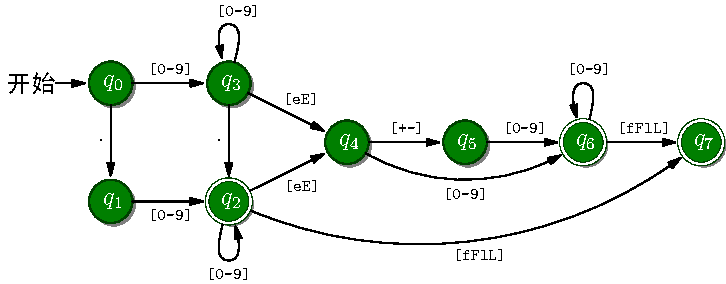
\includegraphics{automata.pdf}
  \caption{最终完成的有限自动机,同\autoref{fig:automata}}
  \label{fig:automatafinal}
\end{figure}

以上就是严教授画出\autoref{fig:automatafinal} 的全部代码。而且,更重要的是,
他为了画出这个有限自动机所做出的各种努力有着比画出这一幅图更多的回报:他可以
继续使用已经完成的 \prgname{simplenode} 模块方便地画出类似的自动机图形,并且
可以扩充这个模块,以完成更丰富的功能。

\section{习题和评注}

\begin{enumerate}
  \item 使用 \Asy{} 本身的 |object| 标签及连线机制,画出下面的状态转移图:
\begin{figure}[H]
  \centering
\begin{asy}
unitsize(2cm);
real margin = 2mm;
currentpen += 0.6;
object  q1 = draw("1", ellipse, (0,0), margin, FillDraw(lightblue)),
        q2 = draw("2", ellipse, (-1,-1), margin, FillDraw(lightblue)),
        q3 = draw("3", ellipse, (1,-1), margin, FillDraw(lightblue));
add(new void(picture pic, transform t) {
    draw(pic, "$\frac14$", point(q1,SW,t) -- point(q2,NE,t), Arrow);
    draw(pic, Label("$\frac34$",LeftSide), point(q1,SE,t) -- point(q3,NW,t),
         Arrow);
    draw(pic, "$\frac12$", point(q2,E,t) -- point(q3,W,t), Arrow);
    draw(pic, "$\frac12$", point(q2,WNW,t){WNW} .. point(q2,W,t)+t*W/4
         .. {-WSW}point(q2,WSW,t), ArcArrow);
    draw(pic, "$1$", point(q3,ESE,t){ESE} .. point(q3,E,t)+t*E/4
         .. {-ENE}point(q3,ENE,t), ArcArrow);
});
\end{asy}
\end{figure}
    注意其中自环箭头的绘制。

    利用 \prgname{simplenode} 重画此图,比较两种方式有什么不同。

  \item (此题较难)查看 \Asy{} 标准模块 \prgname{plain\_filldraw.asy} 中对
    |filltype| 类型的实现,参考 \cite{asyman} 的说明,分析其机制。在 \Asy{}
    1.91 中, |filltype| 被定义为:
\begin{asycode}[numbers=left]
struct filltype 
{
  typedef void fill2(frame f, path[] g, pen fillpen);
  fill2 fill2;
  pen fillpen;
  pen drawpen;

  int type;
  static int Fill=1;
  static int FillDraw=2;
  static int Draw=3;
  static int NoFill=4;
  static int UnFill=5;
      
  void operator init(int type=0, pen fillpen=nullpen, pen drawpen=nullpen,
                     fill2 fill2) {
    this.type=type;
    this.fillpen=fillpen;
    this.drawpen=drawpen;
    this.fill2=fill2;
  }
  void fill(frame f, path[] g, pen p) {fill2(f,g,p);}
}
\end{asycode}
    
    搞清楚:|fill2| 是什么类型?参考 |Fill| 等 |filltype| 填充类型的实现,尤
    其是其中 |RadialShade| 的实现,写一个 |Shadow| 的填充类型,完成前面严教授
    给结点画阴影函数相同的效果。在 \Asy{} 1.90 中 |RadialShade| 被实现为:
\begin{asycode}[numbers=left]
filltype RadialShade(pen penc, pen penr)
{
  return filltype(new void(frame f, path[] g, pen) {
    pair c=(min(g)+max(g))/2;
    radialshade(f,g,penc,c,0,penr,c,abs(max(g)-min(g))/2);
    });
}
\end{asycode}
    其效果是:
\begin{asycode}
object cat
    = draw("cat", ellipse, (0,0), xmargin=2mm, RadialShade(yellow, red));
\end{asycode}
\begin{figure}[H]
  \centering
\begin{asy}
object cat
    = draw("cat", ellipse, (0,0), xmargin=2mm, RadialShade(yellow, red));
\end{asy}
\end{figure}

  \item 仿照前面 |Circle| 函数的实现,为 \prgname{simplenode} 模块增加矩形、
    椭圆、菱形或是其他基本形状结点的构造函数,以便画出更丰富的图形。你可以需
    要一些额外的参数,如文字与边框的距离 |margin|。矩形结点的构造函数原型可以
    是这样的(你可以有不同的做法):
\begin{asycode}
node Rectangle(Label text, pair pos, pen textpen=currentpen,
               real margin=fontsize(textpen)/3, draw_t drawfn);
\end{asycode}
    应该能和 |Circle| 一样方便地使用不同的形状,如:
\begin{asycode}
node cat = Circle("cat", (0,0), filldrawer(yellow)),
     dog = Rectangle("dog", (3cm,0), filler(olive));
draw(cat, dog);
draw(cat .. bendleft .. dog, Arrow);
draw(dog .. bendleft .. cat, Arrow);
\end{asycode}
\begin{figure}[H]
  \centering
\begin{asy}
import "figure-src/simplenode.asy" as simplenode;

node Rectangle(Label text, pair pos, pen textpen=currentpen,
               real margin=fontsize(textpen)/3, draw_t drawfn)
{
    node nd;
    nd.pos = pos;
    label(nd.stuff, text, textpen);
    pair M = max(nd.stuff), m = min(nd.stuff);
    nd.outline = box(m-(margin,margin),M+(margin,margin));
    drawfn(nd.stuff, nd.outline);
    nd.E = nd.dir(E);
    nd.N = nd.dir(N);
    nd.W = nd.dir(W);
    nd.S = nd.dir(S);
    return nd;
}

node cat = Circle("cat", (0,0), filldrawer(yellow)),
     dog = Rectangle("dog", (3cm,0), filler(olive));
draw(cat, dog);
draw(cat .. bendleft .. dog, Arrow);
draw(dog .. bendleft .. cat, Arrow);
\end{asy}
\end{figure}

  \item 模仿 |bendleft|、|bendright| 的定义,为 \prgname{simplenode} 模块扩充
    |edgeconnector| 类型的连线方式。例如,可以增加水平、垂直方向的折线连接
    |HV|,它的用法类似于:
\begin{asycode}
node cat = Circle("cat", (0,0), filldrawer(yellow)),
     dog = Circle("dog", (4cm,3cm), filler(olive));
draw(cat, dog);
draw(cat .. HV .. dog, Arrow);
\end{asycode}
    \begin{figure}[H]
      \centering
\begin{asy}
import "figure-src/simplenode.asy" as simplenode;

path HV(node nd1, node nd2)
{
    path g1 = shift(nd1.pos) * nd1.outline;
    path g2 = shift(nd2.pos) * nd2.outline;
    pair c1 = (max(g1)+min(g1)) / 2;
    pair c2 = (max(g2)+min(g2)) / 2;
    pair z = (c2.x, c1.y);
    path edge = c1 -- z -- c2;
    edge = firstcut(edge, g1).after;
    edge = lastcut(edge, g2).before;
    return edge;
}

node cat = Circle("cat", (0,0), filldrawer(yellow)),
     dog = Circle("dog", (4cm,3cm), filler(olive));
draw(cat, dog);
draw(cat .. HV .. dog, Arrow);
\end{asy}
    \end{figure}
    再定义类似的 |VH|,它先画垂直的线,再画水平的线。(提示:|HV| 和 |VH| 的
    定义可能与 |operator--| 非常相似。)

  \item 在前面实现 |cat .. bendleft .. dog| 这种语法时,严教授使用一个函数作
    为中间类型。事实上也可以使用一个结构体。请补全下面的代码:
\begin{asycode}
typedef path edgeconnector(node nd1, node nd2);

// `\color{comment}中间类型`
struct node_con {
    node nd;
    edgeconnector con;
}

// `\color{comment}nd1 .. con .. nd2 的前一半`
node_con operator..(node nd, edgeconnector con)
{
    // ...
}

// `\color{comment}nd1 .. con .. nd2 的后一半`
path operator..(node_con nc, node nd)
{
    // ...
}
\end{asycode}

  \item 研究记法。
    \begin{enumerate}
      \item 在把多个 |draw_t| 类型的函数复合为一个函数时,严宇教授定义了
        |compose| 函数。但还可以进一步赋予函数复合一种新的记法,如使用加法运
        算符表示复合。试补全下面的实现:
\begin{asycode}
draw_t operator+(draw_t f1, draw_t f2)
{
    // ...
}
\end{asycode}
        并动手试验,能否把加法运算符函数的原型定义这个样子:
\begingroup
\renewcommand\thelstnumber{?}
\begin{asycode}[numbers=left]
draw_t operator+(... draw_t[] fns);
\end{asycode}
\endgroup
        并说明事实上前面定义的二元运算就已经足够了。

      \item 新记法的创立需要符合直观性。前面用加法运算符表示函数的复合函数的
        方式是否符合直观?把加法换成乘法怎么样?

      \item 严教授定义的 |shorten| 函数之所以能方便地使用,一个前提条件是在
        \Asy{} 中 |@| 运算符的优先级比 |--| 和 |..| 要低,因而在变换路径时不
        需要加括号。查阅资料或推测,\Asy{} 中不同运算符的优先级。设计实验并动
        手在 \Asy{} 环境中验证。并考虑在 \Asy{} 中所有可重载的运算符中,各自
        有什么语法特点或限制(能带几个参数、参数类型有没有限制等)。
    \end{enumerate}% 研究记法习题

  \item 严教授已经给出了几种 |draw_t| 的类型:|none|、|drawer|、|filler|、
    |filldrawer|、|shadow| 等等。请扩充 \prgname{simplenode} 中的定义,增加类
    似放射渐变填充类型 |RadialShade| 的效果。想想还有什么可以扩充的,比如说,
    \autoref{sec:object} 中球形立体效果的图形。

  \item\label{ex:flowchart} \Asy{} 的 \prgname{flowchart} 是用来画流程图的一
    个模块。它定义了一种特殊的记法,看起来很像严教授 \prgname{simplenode} 模
    块的用法,也有 \autoref{sec:object} 中 |object| 连线的影子。

    \prgname{flowchart} 
\end{enumerate}

本章的有限自动机及其表示的正则语言,可参看 \cite{aho1974},C 语言词法的形式化
描述参看 \cite{harbison2002}。

在 \Asy{} 中绘制图论图形一直没有很完善的官方模块,以往多是采用
\autoref{sec:object} 一节 |object| 类型的机制绘制的。随 \Asy{} 安装的基本模块
\prgname{flowchart} 是一个专用于绘制流程图的模块,里面定义了 |block| 类型,及
包括矩形、菱形、圆形、圆角矩形、斜多边形(bevel)在内的多种预定义形状,在安装
目录下可以找到例子。1.90 版以前的 \prgname{flowchart} 因为没有采用像本章所采
用的方便的记法,使用的方法与 |object| 类型类似,所以很不方便;自 1.91 版以后
的 \prgname{flowchart} 模块开始支持相对方便的记法了,实现的方法与本章中介绍的
类似。习题~\ref{ex:flowchart} 给出了 \prgname{flowchart} 的相关例子。使用
\prgname{flowchart} 并不足以完成本章带有阴影等修饰和曲线连线的图形,但有可能
扩充这个模板完成类似的功能。

加拿大 Waterloo 大学的博士生 Hubert Chan 曾给出过一个图论模块的框架
\prgname{graphtheory2.asy}(在
\url{http://asymptote.sourceforge.net/links.html} 有介绍),也完成了类似的功
能,并与本章给出的 \prgname{simplenode} 模块有相似,都使用了一些新的记法。

本章的 \prgname{simplenode} 模块是在作者在以前写的一个 \prgname{node} 模块的基
础上简化改编得到的,源代码可以在 \url{http://asy4cn.googlecode.com/} 找到。

本章中 \prgname{simplenode} 的一些设计受 \prgname{Ti\textit{k}Z} 宏包的影响,
参看 \cite{pgfman}。


\endinput

% vim:tw=77:



\appendix
\chapter{GNU GENERAL PUBLIC LICENSE}
\label{chap:license}

\begin{center}
{\parindent 0in

Version 3, 29 June 2007

Copyright \copyright\  2007 Free Software Foundation, Inc. \texttt{http://fsf.org/}

\bigskip
Everyone is permitted to copy and distribute verbatim copies of this

license document, but changing it is not allowed.}

\end{center}


\section{Preamble}

The GNU General Public License is a free, copyleft license for
software and other kinds of works.

The licenses for most software and other practical works are designed
to take away your freedom to share and change the works.  By contrast,
the GNU General Public License is intended to guarantee your freedom to
share and change all versions of a program--to make sure it remains free
software for all its users.  We, the Free Software Foundation, use the
GNU General Public License for most of our software; it applies also to
any other work released this way by its authors.  You can apply it to
your programs, too.

When we speak of free software, we are referring to freedom, not
price.  Our General Public Licenses are designed to make sure that you
have the freedom to distribute copies of free software (and charge for
them if you wish), that you receive source code or can get it if you
want it, that you can change the software or use pieces of it in new
free programs, and that you know you can do these things.

To protect your rights, we need to prevent others from denying you
these rights or asking you to surrender the rights.  Therefore, you have
certain responsibilities if you distribute copies of the software, or if
you modify it: responsibilities to respect the freedom of others.

For example, if you distribute copies of such a program, whether
gratis or for a fee, you must pass on to the recipients the same
freedoms that you received.  You must make sure that they, too, receive
or can get the source code.  And you must show them these terms so they
know their rights.

Developers that use the GNU GPL protect your rights with two steps:
(1) assert copyright on the software, and (2) offer you this License
giving you legal permission to copy, distribute and/or modify it.

For the developers' and authors' protection, the GPL clearly explains
that there is no warranty for this free software.  For both users' and
authors' sake, the GPL requires that modified versions be marked as
changed, so that their problems will not be attributed erroneously to
authors of previous versions.

Some devices are designed to deny users access to install or run
modified versions of the software inside them, although the manufacturer
can do so.  This is fundamentally incompatible with the aim of
protecting users' freedom to change the software.  The systematic
pattern of such abuse occurs in the area of products for individuals to
use, which is precisely where it is most unacceptable.  Therefore, we
have designed this version of the GPL to prohibit the practice for those
products.  If such problems arise substantially in other domains, we
stand ready to extend this provision to those domains in future versions
of the GPL, as needed to protect the freedom of users.

Finally, every program is threatened constantly by software patents.
States should not allow patents to restrict development and use of
software on general-purpose computers, but in those that do, we wish to
avoid the special danger that patents applied to a free program could
make it effectively proprietary.  To prevent this, the GPL assures that
patents cannot be used to render the program non-free.

The precise terms and conditions for copying, distribution and
modification follow.


\section{Terms and Conditions}


\begin{enumerate}

\addtocounter{enumi}{-1}

\item Definitions.

``This License'' refers to version 3 of the GNU General Public License.

``Copyright'' also means copyright-like laws that apply to other kinds of
works, such as semiconductor masks.

``The Program'' refers to any copyrightable work licensed under this
License.  Each licensee is addressed as ``you''.  ``Licensees'' and
``recipients'' may be individuals or organizations.

To ``modify'' a work means to copy from or adapt all or part of the work
in a fashion requiring copyright permission, other than the making of an
exact copy.  The resulting work is called a ``modified version'' of the
earlier work or a work ``based on'' the earlier work.

A ``covered work'' means either the unmodified Program or a work based
on the Program.

To ``propagate'' a work means to do anything with it that, without
permission, would make you directly or secondarily liable for
infringement under applicable copyright law, except executing it on a
computer or modifying a private copy.  Propagation includes copying,
distribution (with or without modification), making available to the
public, and in some countries other activities as well.

To ``convey'' a work means any kind of propagation that enables other
parties to make or receive copies.  Mere interaction with a user through
a computer network, with no transfer of a copy, is not conveying.

An interactive user interface displays ``Appropriate Legal Notices''
to the extent that it includes a convenient and prominently visible
feature that (1) displays an appropriate copyright notice, and (2)
tells the user that there is no warranty for the work (except to the
extent that warranties are provided), that licensees may convey the
work under this License, and how to view a copy of this License.  If
the interface presents a list of user commands or options, such as a
menu, a prominent item in the list meets this criterion.

\item Source Code.

The ``source code'' for a work means the preferred form of the work
for making modifications to it.  ``Object code'' means any non-source
form of a work.

A ``Standard Interface'' means an interface that either is an official
standard defined by a recognized standards body, or, in the case of
interfaces specified for a particular programming language, one that
is widely used among developers working in that language.

The ``System Libraries'' of an executable work include anything, other
than the work as a whole, that (a) is included in the normal form of
packaging a Major Component, but which is not part of that Major
Component, and (b) serves only to enable use of the work with that
Major Component, or to implement a Standard Interface for which an
implementation is available to the public in source code form.  A
``Major Component'', in this context, means a major essential component
(kernel, window system, and so on) of the specific operating system
(if any) on which the executable work runs, or a compiler used to
produce the work, or an object code interpreter used to run it.

The ``Corresponding Source'' for a work in object code form means all
the source code needed to generate, install, and (for an executable
work) run the object code and to modify the work, including scripts to
control those activities.  However, it does not include the work's
System Libraries, or general-purpose tools or generally available free
programs which are used unmodified in performing those activities but
which are not part of the work.  For example, Corresponding Source
includes interface definition files associated with source files for
the work, and the source code for shared libraries and dynamically
linked subprograms that the work is specifically designed to require,
such as by intimate data communication or control flow between those
subprograms and other parts of the work.

The Corresponding Source need not include anything that users
can regenerate automatically from other parts of the Corresponding
Source.

The Corresponding Source for a work in source code form is that
same work.

\item Basic Permissions.

All rights granted under this License are granted for the term of
copyright on the Program, and are irrevocable provided the stated
conditions are met.  This License explicitly affirms your unlimited
permission to run the unmodified Program.  The output from running a
covered work is covered by this License only if the output, given its
content, constitutes a covered work.  This License acknowledges your
rights of fair use or other equivalent, as provided by copyright law.

You may make, run and propagate covered works that you do not
convey, without conditions so long as your license otherwise remains
in force.  You may convey covered works to others for the sole purpose
of having them make modifications exclusively for you, or provide you
with facilities for running those works, provided that you comply with
the terms of this License in conveying all material for which you do
not control copyright.  Those thus making or running the covered works
for you must do so exclusively on your behalf, under your direction
and control, on terms that prohibit them from making any copies of
your copyrighted material outside their relationship with you.

Conveying under any other circumstances is permitted solely under
the conditions stated below.  Sublicensing is not allowed; section 10
makes it unnecessary.

\item Protecting Users' Legal Rights From Anti-Circumvention Law.

No covered work shall be deemed part of an effective technological
measure under any applicable law fulfilling obligations under article
11 of the WIPO copyright treaty adopted on 20 December 1996, or
similar laws prohibiting or restricting circumvention of such
measures.

When you convey a covered work, you waive any legal power to forbid
circumvention of technological measures to the extent such circumvention
is effected by exercising rights under this License with respect to
the covered work, and you disclaim any intention to limit operation or
modification of the work as a means of enforcing, against the work's
users, your or third parties' legal rights to forbid circumvention of
technological measures.

\item Conveying Verbatim Copies.

You may convey verbatim copies of the Program's source code as you
receive it, in any medium, provided that you conspicuously and
appropriately publish on each copy an appropriate copyright notice;
keep intact all notices stating that this License and any
non-permissive terms added in accord with section 7 apply to the code;
keep intact all notices of the absence of any warranty; and give all
recipients a copy of this License along with the Program.

You may charge any price or no price for each copy that you convey,
and you may offer support or warranty protection for a fee.

\item Conveying Modified Source Versions.

You may convey a work based on the Program, or the modifications to
produce it from the Program, in the form of source code under the
terms of section 4, provided that you also meet all of these conditions:
  \begin{enumerate}
  \item The work must carry prominent notices stating that you modified
  it, and giving a relevant date.

  \item The work must carry prominent notices stating that it is
  released under this License and any conditions added under section
  7.  This requirement modifies the requirement in section 4 to
  ``keep intact all notices''.

  \item You must license the entire work, as a whole, under this
  License to anyone who comes into possession of a copy.  This
  License will therefore apply, along with any applicable section 7
  additional terms, to the whole of the work, and all its parts,
  regardless of how they are packaged.  This License gives no
  permission to license the work in any other way, but it does not
  invalidate such permission if you have separately received it.

  \item If the work has interactive user interfaces, each must display
  Appropriate Legal Notices; however, if the Program has interactive
  interfaces that do not display Appropriate Legal Notices, your
  work need not make them do so.
\end{enumerate}
A compilation of a covered work with other separate and independent
works, which are not by their nature extensions of the covered work,
and which are not combined with it such as to form a larger program,
in or on a volume of a storage or distribution medium, is called an
``aggregate'' if the compilation and its resulting copyright are not
used to limit the access or legal rights of the compilation's users
beyond what the individual works permit.  Inclusion of a covered work
in an aggregate does not cause this License to apply to the other
parts of the aggregate.

\item Conveying Non-Source Forms.

You may convey a covered work in object code form under the terms
of sections 4 and 5, provided that you also convey the
machine-readable Corresponding Source under the terms of this License,
in one of these ways:
  \begin{enumerate}
  \item Convey the object code in, or embodied in, a physical product
  (including a physical distribution medium), accompanied by the
  Corresponding Source fixed on a durable physical medium
  customarily used for software interchange.

  \item Convey the object code in, or embodied in, a physical product
  (including a physical distribution medium), accompanied by a
  written offer, valid for at least three years and valid for as
  long as you offer spare parts or customer support for that product
  model, to give anyone who possesses the object code either (1) a
  copy of the Corresponding Source for all the software in the
  product that is covered by this License, on a durable physical
  medium customarily used for software interchange, for a price no
  more than your reasonable cost of physically performing this
  conveying of source, or (2) access to copy the
  Corresponding Source from a network server at no charge.

  \item Convey individual copies of the object code with a copy of the
  written offer to provide the Corresponding Source.  This
  alternative is allowed only occasionally and noncommercially, and
  only if you received the object code with such an offer, in accord
  with subsection 6b.

  \item Convey the object code by offering access from a designated
  place (gratis or for a charge), and offer equivalent access to the
  Corresponding Source in the same way through the same place at no
  further charge.  You need not require recipients to copy the
  Corresponding Source along with the object code.  If the place to
  copy the object code is a network server, the Corresponding Source
  may be on a different server (operated by you or a third party)
  that supports equivalent copying facilities, provided you maintain
  clear directions next to the object code saying where to find the
  Corresponding Source.  Regardless of what server hosts the
  Corresponding Source, you remain obligated to ensure that it is
  available for as long as needed to satisfy these requirements.

  \item Convey the object code using peer-to-peer transmission, provided
  you inform other peers where the object code and Corresponding
  Source of the work are being offered to the general public at no
  charge under subsection 6d.
  \end{enumerate}

A separable portion of the object code, whose source code is excluded
from the Corresponding Source as a System Library, need not be
included in conveying the object code work.

A ``User Product'' is either (1) a ``consumer product'', which means any
tangible personal property which is normally used for personal, family,
or household purposes, or (2) anything designed or sold for incorporation
into a dwelling.  In determining whether a product is a consumer product,
doubtful cases shall be resolved in favor of coverage.  For a particular
product received by a particular user, ``normally used'' refers to a
typical or common use of that class of product, regardless of the status
of the particular user or of the way in which the particular user
actually uses, or expects or is expected to use, the product.  A product
is a consumer product regardless of whether the product has substantial
commercial, industrial or non-consumer uses, unless such uses represent
the only significant mode of use of the product.

``Installation Information'' for a User Product means any methods,
procedures, authorization keys, or other information required to install
and execute modified versions of a covered work in that User Product from
a modified version of its Corresponding Source.  The information must
suffice to ensure that the continued functioning of the modified object
code is in no case prevented or interfered with solely because
modification has been made.

If you convey an object code work under this section in, or with, or
specifically for use in, a User Product, and the conveying occurs as
part of a transaction in which the right of possession and use of the
User Product is transferred to the recipient in perpetuity or for a
fixed term (regardless of how the transaction is characterized), the
Corresponding Source conveyed under this section must be accompanied
by the Installation Information.  But this requirement does not apply
if neither you nor any third party retains the ability to install
modified object code on the User Product (for example, the work has
been installed in ROM).

The requirement to provide Installation Information does not include a
requirement to continue to provide support service, warranty, or updates
for a work that has been modified or installed by the recipient, or for
the User Product in which it has been modified or installed.  Access to a
network may be denied when the modification itself materially and
adversely affects the operation of the network or violates the rules and
protocols for communication across the network.

Corresponding Source conveyed, and Installation Information provided,
in accord with this section must be in a format that is publicly
documented (and with an implementation available to the public in
source code form), and must require no special password or key for
unpacking, reading or copying.

\item Additional Terms.

``Additional permissions'' are terms that supplement the terms of this
License by making exceptions from one or more of its conditions.
Additional permissions that are applicable to the entire Program shall
be treated as though they were included in this License, to the extent
that they are valid under applicable law.  If additional permissions
apply only to part of the Program, that part may be used separately
under those permissions, but the entire Program remains governed by
this License without regard to the additional permissions.

When you convey a copy of a covered work, you may at your option
remove any additional permissions from that copy, or from any part of
it.  (Additional permissions may be written to require their own
removal in certain cases when you modify the work.)  You may place
additional permissions on material, added by you to a covered work,
for which you have or can give appropriate copyright permission.

Notwithstanding any other provision of this License, for material you
add to a covered work, you may (if authorized by the copyright holders of
that material) supplement the terms of this License with terms:
  \begin{enumerate}
  \item Disclaiming warranty or limiting liability differently from the
  terms of sections 15 and 16 of this License; or

  \item Requiring preservation of specified reasonable legal notices or
  author attributions in that material or in the Appropriate Legal
  Notices displayed by works containing it; or

  \item Prohibiting misrepresentation of the origin of that material, or
  requiring that modified versions of such material be marked in
  reasonable ways as different from the original version; or

  \item Limiting the use for publicity purposes of names of licensors or
  authors of the material; or

  \item Declining to grant rights under trademark law for use of some
  trade names, trademarks, or service marks; or

  \item Requiring indemnification of licensors and authors of that
  material by anyone who conveys the material (or modified versions of
  it) with contractual assumptions of liability to the recipient, for
  any liability that these contractual assumptions directly impose on
  those licensors and authors.
  \end{enumerate}

All other non-permissive additional terms are considered ``further
restrictions'' within the meaning of section 10.  If the Program as you
received it, or any part of it, contains a notice stating that it is
governed by this License along with a term that is a further
restriction, you may remove that term.  If a license document contains
a further restriction but permits relicensing or conveying under this
License, you may add to a covered work material governed by the terms
of that license document, provided that the further restriction does
not survive such relicensing or conveying.

If you add terms to a covered work in accord with this section, you
must place, in the relevant source files, a statement of the
additional terms that apply to those files, or a notice indicating
where to find the applicable terms.

Additional terms, permissive or non-permissive, may be stated in the
form of a separately written license, or stated as exceptions;
the above requirements apply either way.

\item Termination.

You may not propagate or modify a covered work except as expressly
provided under this License.  Any attempt otherwise to propagate or
modify it is void, and will automatically terminate your rights under
this License (including any patent licenses granted under the third
paragraph of section 11).

However, if you cease all violation of this License, then your
license from a particular copyright holder is reinstated (a)
provisionally, unless and until the copyright holder explicitly and
finally terminates your license, and (b) permanently, if the copyright
holder fails to notify you of the violation by some reasonable means
prior to 60 days after the cessation.

Moreover, your license from a particular copyright holder is
reinstated permanently if the copyright holder notifies you of the
violation by some reasonable means, this is the first time you have
received notice of violation of this License (for any work) from that
copyright holder, and you cure the violation prior to 30 days after
your receipt of the notice.

Termination of your rights under this section does not terminate the
licenses of parties who have received copies or rights from you under
this License.  If your rights have been terminated and not permanently
reinstated, you do not qualify to receive new licenses for the same
material under section 10.

\item Acceptance Not Required for Having Copies.

You are not required to accept this License in order to receive or
run a copy of the Program.  Ancillary propagation of a covered work
occurring solely as a consequence of using peer-to-peer transmission
to receive a copy likewise does not require acceptance.  However,
nothing other than this License grants you permission to propagate or
modify any covered work.  These actions infringe copyright if you do
not accept this License.  Therefore, by modifying or propagating a
covered work, you indicate your acceptance of this License to do so.

\item Automatic Licensing of Downstream Recipients.

Each time you convey a covered work, the recipient automatically
receives a license from the original licensors, to run, modify and
propagate that work, subject to this License.  You are not responsible
for enforcing compliance by third parties with this License.

An ``entity transaction'' is a transaction transferring control of an
organization, or substantially all assets of one, or subdividing an
organization, or merging organizations.  If propagation of a covered
work results from an entity transaction, each party to that
transaction who receives a copy of the work also receives whatever
licenses to the work the party's predecessor in interest had or could
give under the previous paragraph, plus a right to possession of the
Corresponding Source of the work from the predecessor in interest, if
the predecessor has it or can get it with reasonable efforts.

You may not impose any further restrictions on the exercise of the
rights granted or affirmed under this License.  For example, you may
not impose a license fee, royalty, or other charge for exercise of
rights granted under this License, and you may not initiate litigation
(including a cross-claim or counterclaim in a lawsuit) alleging that
any patent claim is infringed by making, using, selling, offering for
sale, or importing the Program or any portion of it.

\item Patents.

A ``contributor'' is a copyright holder who authorizes use under this
License of the Program or a work on which the Program is based.  The
work thus licensed is called the contributor's ``contributor version''.

A contributor's ``essential patent claims'' are all patent claims
owned or controlled by the contributor, whether already acquired or
hereafter acquired, that would be infringed by some manner, permitted
by this License, of making, using, or selling its contributor version,
but do not include claims that would be infringed only as a
consequence of further modification of the contributor version.  For
purposes of this definition, ``control'' includes the right to grant
patent sublicenses in a manner consistent with the requirements of
this License.

Each contributor grants you a non-exclusive, worldwide, royalty-free
patent license under the contributor's essential patent claims, to
make, use, sell, offer for sale, import and otherwise run, modify and
propagate the contents of its contributor version.

In the following three paragraphs, a ``patent license'' is any express
agreement or commitment, however denominated, not to enforce a patent
(such as an express permission to practice a patent or covenant not to
sue for patent infringement).  To ``grant'' such a patent license to a
party means to make such an agreement or commitment not to enforce a
patent against the party.

If you convey a covered work, knowingly relying on a patent license,
and the Corresponding Source of the work is not available for anyone
to copy, free of charge and under the terms of this License, through a
publicly available network server or other readily accessible means,
then you must either (1) cause the Corresponding Source to be so
available, or (2) arrange to deprive yourself of the benefit of the
patent license for this particular work, or (3) arrange, in a manner
consistent with the requirements of this License, to extend the patent
license to downstream recipients.  ``Knowingly relying'' means you have
actual knowledge that, but for the patent license, your conveying the
covered work in a country, or your recipient's use of the covered work
in a country, would infringe one or more identifiable patents in that
country that you have reason to believe are valid.

If, pursuant to or in connection with a single transaction or
arrangement, you convey, or propagate by procuring conveyance of, a
covered work, and grant a patent license to some of the parties
receiving the covered work authorizing them to use, propagate, modify
or convey a specific copy of the covered work, then the patent license
you grant is automatically extended to all recipients of the covered
work and works based on it.

A patent license is ``discriminatory'' if it does not include within
the scope of its coverage, prohibits the exercise of, or is
conditioned on the non-exercise of one or more of the rights that are
specifically granted under this License.  You may not convey a covered
work if you are a party to an arrangement with a third party that is
in the business of distributing software, under which you make payment
to the third party based on the extent of your activity of conveying
the work, and under which the third party grants, to any of the
parties who would receive the covered work from you, a discriminatory
patent license (a) in connection with copies of the covered work
conveyed by you (or copies made from those copies), or (b) primarily
for and in connection with specific products or compilations that
contain the covered work, unless you entered into that arrangement,
or that patent license was granted, prior to 28 March 2007.

Nothing in this License shall be construed as excluding or limiting
any implied license or other defenses to infringement that may
otherwise be available to you under applicable patent law.

\item No Surrender of Others' Freedom.

If conditions are imposed on you (whether by court order, agreement or
otherwise) that contradict the conditions of this License, they do not
excuse you from the conditions of this License.  If you cannot convey a
covered work so as to satisfy simultaneously your obligations under this
License and any other pertinent obligations, then as a consequence you may
not convey it at all.  For example, if you agree to terms that obligate you
to collect a royalty for further conveying from those to whom you convey
the Program, the only way you could satisfy both those terms and this
License would be to refrain entirely from conveying the Program.

\item Use with the GNU Affero General Public License.

Notwithstanding any other provision of this License, you have
permission to link or combine any covered work with a work licensed
under version 3 of the GNU Affero General Public License into a single
combined work, and to convey the resulting work.  The terms of this
License will continue to apply to the part which is the covered work,
but the special requirements of the GNU Affero General Public License,
section 13, concerning interaction through a network will apply to the
combination as such.

\item Revised Versions of this License.

The Free Software Foundation may publish revised and/or new versions of
the GNU General Public License from time to time.  Such new versions will
be similar in spirit to the present version, but may differ in detail to
address new problems or concerns.

Each version is given a distinguishing version number.  If the
Program specifies that a certain numbered version of the GNU General
Public License ``or any later version'' applies to it, you have the
option of following the terms and conditions either of that numbered
version or of any later version published by the Free Software
Foundation.  If the Program does not specify a version number of the
GNU General Public License, you may choose any version ever published
by the Free Software Foundation.

If the Program specifies that a proxy can decide which future
versions of the GNU General Public License can be used, that proxy's
public statement of acceptance of a version permanently authorizes you
to choose that version for the Program.

Later license versions may give you additional or different
permissions.  However, no additional obligations are imposed on any
author or copyright holder as a result of your choosing to follow a
later version.

\item Disclaimer of Warranty.

\begin{sloppypar}
 THERE IS NO WARRANTY FOR THE PROGRAM, TO THE EXTENT PERMITTED BY
 APPLICABLE LAW.  EXCEPT WHEN OTHERWISE STATED IN WRITING THE
 COPYRIGHT HOLDERS AND/OR OTHER PARTIES PROVIDE THE PROGRAM ``AS IS''
 WITHOUT WARRANTY OF ANY KIND, EITHER EXPRESSED OR IMPLIED,
 INCLUDING, BUT NOT LIMITED TO, THE IMPLIED WARRANTIES OF
 MERCHANTABILITY AND FITNESS FOR A PARTICULAR PURPOSE.  THE ENTIRE
 RISK AS TO THE QUALITY AND PERFORMANCE OF THE PROGRAM IS WITH YOU.
 SHOULD THE PROGRAM PROVE DEFECTIVE, YOU ASSUME THE COST OF ALL
 NECESSARY SERVICING, REPAIR OR CORRECTION.
\end{sloppypar}

\item Limitation of Liability.

 IN NO EVENT UNLESS REQUIRED BY APPLICABLE LAW OR AGREED TO IN
 WRITING WILL ANY COPYRIGHT HOLDER, OR ANY OTHER PARTY WHO MODIFIES
 AND/OR CONVEYS THE PROGRAM AS PERMITTED ABOVE, BE LIABLE TO YOU FOR
 DAMAGES, INCLUDING ANY GENERAL, SPECIAL, INCIDENTAL OR CONSEQUENTIAL
 DAMAGES ARISING OUT OF THE USE OR INABILITY TO USE THE PROGRAM
 (INCLUDING BUT NOT LIMITED TO LOSS OF DATA OR DATA BEING RENDERED
 INACCURATE OR LOSSES SUSTAINED BY YOU OR THIRD PARTIES OR A FAILURE
 OF THE PROGRAM TO OPERATE WITH ANY OTHER PROGRAMS), EVEN IF SUCH
 HOLDER OR OTHER PARTY HAS BEEN ADVISED OF THE POSSIBILITY OF SUCH
 DAMAGES.

\item Interpretation of Sections 15 and 16.

If the disclaimer of warranty and limitation of liability provided
above cannot be given local legal effect according to their terms,
reviewing courts shall apply local law that most closely approximates
an absolute waiver of all civil liability in connection with the
Program, unless a warranty or assumption of liability accompanies a
copy of the Program in return for a fee.

\end{enumerate}


\section{End of Terms and Conditions}

\begin{center}
How to Apply These Terms to Your New Programs
\end{center}

If you develop a new program, and you want it to be of the greatest
possible use to the public, the best way to achieve this is to make it
free software which everyone can redistribute and change under these terms.

To do so, attach the following notices to the program.  It is safest
to attach them to the start of each source file to most effectively
state the exclusion of warranty; and each file should have at least
the ``copyright'' line and a pointer to where the full notice is found.

{\footnotesize
\begin{verbatim}
<one line to give the program's name and a brief idea of what it does.>

Copyright (C) <textyear>  <name of author>

This program is free software: you can redistribute it and/or modify
it under the terms of the GNU General Public License as published by
the Free Software Foundation, either version 3 of the License, or
(at your option) any later version.

This program is distributed in the hope that it will be useful,
but WITHOUT ANY WARRANTY; without even the implied warranty of
MERCHANTABILITY or FITNESS FOR A PARTICULAR PURPOSE.  See the
GNU General Public License for more details.

You should have received a copy of the GNU General Public License
along with this program.  If not, see <http://www.gnu.org/licenses/>.
\end{verbatim}
}

Also add information on how to contact you by electronic and paper mail.

If the program does terminal interaction, make it output a short
notice like this when it starts in an interactive mode:

{\footnotesize
\begin{verbatim}
<program>  Copyright (C) <year>  <name of author>

This program comes with ABSOLUTELY NO WARRANTY; for details type `show w'.
This is free software, and you are welcome to redistribute it
under certain conditions; type `show c' for details.
\end{verbatim}
}

The hypothetical commands {\tt show w} and {\tt show c} should show
the appropriate
parts of the General Public License.  Of course, your program's commands
might be different; for a GUI interface, you would use an ``about box''.

You should also get your employer (if you work as a programmer) or
school, if any, to sign a ``copyright disclaimer'' for the program, if
necessary.  For more information on this, and how to apply and follow
the GNU GPL, see \texttt{http://www.gnu.org/licenses/}.

The GNU General Public License does not permit incorporating your
program into proprietary programs.  If your program is a subroutine
library, you may consider it more useful to permit linking proprietary
applications with the library.  If this is what you want to do, use
the GNU Lesser General Public License instead of this License.  But
first, please read \texttt{http://www.gnu.org/philosophy/why-not-lgpl.html}.


\endinput


\printindex

\bibliographystyle{plain}
\bibliography{asy}
\end{document}
